\documentclass[12pt,a4paper]{book}

\usepackage [english]{babel}
\usepackage [utf8]{inputenc}

%\usepackage[left=2.5cm,right=2.5cm,top=2.5cm,bottom=2.5cm]{geometry}

\usepackage{longtable}
 
%\setcounter{secnumdepth}{3} % le estoy indicando la profundidad hasta donde tiene que mostrar en el indice
%\setcounter{tocdepth}{4} 

\usepackage[titletoc]{appendix}

\RequirePackage[paperwidth=17cm,paperheight=24cm,inner=15mm,outer=20mm,top=25mm,bottom=25mm]{geometry} %%dimensiones externas del pdf y margenes internos.

\usepackage [T1]{fontenc}
\usepackage{graphicx}
\usepackage{graphics}
\graphicspath{ {Figures/} } %Para buscar las imágenes en otra carpeta
\usepackage{amsfonts} %Para poder escribir letras como la matriz identidad
\usepackage{mathrsfs} %Para poder escribir letras como la H del el espacio de Hilbert
\usepackage{slashed} % para la barra cruzada
\usepackage{amsmath}
\usepackage{amssymb}
\usepackage{makeidx}
\usepackage{hepunits} %para poder utilizar unidades
\usepackage[version=3]{mhchem} %para poder escribir los simpolos atómicos y químicos
%\usepackage{hep}

%\renewcommand{\figurename}{ Figura}
%\usepackage[labelsep=endash]{caption}

%\usepackage[figurename=\bold{Figura}]{caption}
%\usepackage [labelformat=empty]{caption}
%\usepackage{wrapfig} %for I can use wrapfigure
\usepackage[font={small, up}]{caption}
\usepackage[caption = false]{subfig} %% for putting several pictures in the same line
\usepackage{hyperref} %hipervinculos del índice
\setlength{\parindent}{4em} %para que interprete la linea en blanco como un \parragraph{}
\setlength{\parskip}{1em}
%\usepackage{subcaption}
%\usepackage[caption = false]{subfig}


\renewcommand{\baselinestretch}{1.15}
%\renewcommand{\thefigure}{}

%para aumentar el espacio entre elementos del índice
\usepackage{setspace}

\bibliographystyle{unsrthep}



\begin{document}
\captionsetup[figure]{labelfont={bf},labelformat={default},labelsep= endash,name={Figura}}
\begin{titlepage}

\begin{center}
%\vspace*{-1 cm}
%\vspace*{1 cm}
%%\begin{figure}[htb]
%%\begin{center}
%%
\includegraphics[scale=0.7]{1Cover_page/Logo1.png}
%%\end{center}
%%\end{figure}
%%\vspace*{0.2 cm}


%\vspace*{0.2in}
{\large Facultad de Física}\\
{\large Departamento de Fisica Atómica, Molecular y Nuclear}\\
\vspace*{0.2in}
\vspace*{0.6in}
\end{center}
\vspace*{-1in}
\begin{center}
\vspace*{1 cm}


\begin{figure}[htb]
\begin{center}

\includegraphics[scale=0.06]{1Cover_page/Logo2.jpg} 
\end{center}
\end{figure}
\vspace*{1 cm}

\begin{large}
%%\textbf{{\large Thesis}}\\
%%\rule{80mm}{0.1mm}\\
%\vspace*{2 cm}

\end{large}
%%\vspace*{0.2 cm}
\begin{Large}
\textbf{\LARGE TRITIUM: Design, Construction and Commissioning of an In-Water Tritium Detector} \\
\end{Large}
%\vspace*{0.3in}
\vspace*{1.2 cm}

\begin{large}
\textbf{Marcos Martínez Roig}\\
Ph.D. Dissertation\\
\today
\end{large}
\end{center}

\vspace*{-1.2 cm}
%\rule{80mm}{0.1mm}\\
%\vspace*{0.1in}
%\begin{large}
\begin{flushright}
\item[\bf Under the supervison of:]\quad  \\ 
José Díaz Medina\\
Nadia Yahlali Haddou\\
\end{flushright}
%\end{large}

\end{titlepage}


$\ $
\thispagestyle{empty}  %para que no se numere esta pagina
\chapter*{} 

\pagenumbering{Roman} %for using romain numbers (page numering)


\begin{flushright}
\textit{Dedicated to \\my family}
\end{flushright} 

\vspace{10cm}

\begin{flushleft}
Sometimes it's the people no one imagines anything \\
of whom do the things that no one can imagine.
\end{flushleft} 
\begin{flushright}
\textbf{"Alan Turing"}
\end{flushright} 


\newpage

\chapter*{Acknowledgements} \label{chap:Acknowledgements}  %pongo el asterisco para que no se numere ni aparezca en el índice
%%\cleardoublepage
\addcontentsline{toc}{chapter}{Acknowledgements} % para que aparezca en el indice de contenidos
%%\vspace{-1.2cm}
Al echar la mirada atrás a estos años de trabajo y formación como investigadora, siento que ha habido muchas personas que me han ayudado directa o indirectamente en esta aventura, por lo que no puede faltar este espacio para agradecer la ayuda que he recibido.

Durante estos 4 años han sido muchas las personas que me han ayudado. Espero no dejarme a nadie.

Ver memoria de "Detectores monolíticos y sensores compatibles con altos campos magnéticos para tomografía por emisión de positrones"


AGRADECER A:

\begin{itemize}
\item{} Gente de tritium Valencia: PEPE, NADIA, MIREIA, ANA, MARQUITOS, ANDREA.
\item{} Gente del LARAM -> TERESA, VANESA, ROSA, CLODO
\item{} Gente de Tritium -> GENTE DE PORTUGAL, Antonio y Jose Angel de extremadura, gente de francia...  
\item{} Gente que ha aportado al trabajo:
\begin{itemize}
\item{} Gente de DUNE (Anselmo, Miguel, Justo)
\item{} Gente de NEXT (Vicente, Marc, Javier, la chica, etc...)
\item{} Ingeniero electrónico David Calvo del IFIC
\item{} Gente del IFIMED (Ana Ros, Jhon Barrio y Gabriela Llosa del IFIMED, Rita, Jorge, Marina)
\item{} Gente de Espectrometría Gamma (El hombre y su mujer, Cesar, Ion, el doctorado, etc)
\item{} Gente de ATLAS (Urmila, Carlos Mariñas)
\item{} Gente del ICMOL (El que manda, Lidon)
\item{} Departamento de mecánica del IFIC (Manolo "Apellidos", Jose Luis Jordan, Jose Vicente Civera Navarrete, Tchogna Davis, Daniel)
\item{} departamento de electrónica del IFIC (Jorge Nacher Arándiga, Manu ... y el otro )
\item{} Al departamento de informática (gente)
\end{itemize}
\item{} Gente externa que ha ayudado
\begin{itemize}
\item{} DAVID CANAL DE SAMTEC
\item{} A LUIS FERR... DE PETSYS..
\end{itemize}
\item{} Gente externa que no ha ayudado
\begin{itemize}
\item{} Grupo de amigos del IFIC (nombrar a todos, tanto en el master como en el doctorado)
\item{} Familia
\item{} Amigos del pueblo
\end{itemize}
\item{} Al programa interreg sudoe -> Soporte financiero!
\end{itemize} 





\newpage

\chapter*{Abstract} \label{chap:Abstract}
%%\cleardoublepage
\addcontentsline{toc}{chapter}{Abstract} % para que aparezca en el indice de contenidos
Tritium is one of the most frequently emitted radioisotopes in a nuclear power plant. Large quantities of tritium are normally produced in the water of their cooling system, which are finally emitted to the environment. Due to the fact that high quantities of tritium could be dangerous for human health and for the environment, there exist several legislations around the world which try to control this radioactive emissions in each country, like the Directive Europeen 2013/51/Euratom, which establishes the tritium limit in drinking water in Europe at $100~\becquerel/\liter$, or the U. S. Environmental Protection Agency, in United States, whose tritium limit in drinking water is established at $740~\becquerel/\liter$.

Nowadays, due to such a low energy emitted in the tritium decay, we need high sensitive detectors for measuring it like LSC. The problem with LSC is that it is a off-line method whose measurement process can take up to 3 or 4 days, too much time if there are any problem with the NPP.

Detectors based on solid scintillators is a promissing idea for building a tritium detector that works in quasi-real time. This type of detectors has been developed so far succesfully but without achieving enough sensibility for measuring the legal limits.

In this study the results of TRITIUM project is presented. In the framework of this project we have developed a quasi-real time monitor for low tritium activities in water. This monitor is based on a tritium detector that contains several detection cells which we read in parallel, several active vetos and a pasive shielding for reduce the natural background of our system and an ultrapure water system to prepare the sample before we measure. Each detection cell is made up of hundreds of scintillating fibers read out by PMTs or SiPM arrays.

The final objective of this monitor will be the radiological protection around the nuclear power plant. This monitor will provide an alarm in case of an unexpected tritium release. It will be included in the early alarm system of Extremadura consisting of several detectors whose objective is to reduce the impact of Nuclear Power Plants to the environment.

\vspace{1cm}

\textbf{Keywords:} Tritium in water, Real-time monitor, Nuclear Power Plant, ENvironmental Safety, ...

%\begin{abstract}
%Texto           del           abstract
%\end{abstract}

\newpage

\chapter*{Nomenclature and Acronyms} \label{chap:NomenclatureAcronyms}  %pongo el asterisco para que no se numere ni aparezca en el índice
%%\cleardoublepage
\addcontentsline{toc}{chapter}{Nomenclature and acronyms} % para que aparezca en el indice de contenidos
\begin{longtable}{p{25mm} c p{120mm} }
\multicolumn{3}{l}{Acronyms:}\\
\\
$ALARA$ & --- & As low as reasonably achievable criterium\\
$APD$ & --- & Avalanche photodiode\\
$BIXS$ & --- & Beta induced X-ray spectrometry\\
$BWR$ & --- & Boiling water reactor\\
$CCD$ & --- & Charge-coupled device\\
$CDF$ & --- & Dose conversion factor\\
$CE$ & --- & Collection efficiency\\
$CNRS$ & --- & Le Centre National de la Recherche Scientifique, France\\
$CSN$ & --- & Consejo de Seguridad Nuclear\\
$C_t$ & --- & Terminal capacitance of SiPM\\
$DAQ$ & --- & Data acquisition system\\
$DRIM$ & --- & Deteç$\tilde{\text{a}}$o da Radiaç$\tilde{\text{a}}$o e Laboratorio Imagem Médica
\newline
(Laboratory for Radiation Detection and 
\newline
Medical Imaging)\\
$EEC$ & --- & European Economical Community\\
$EPA$ & --- & Environmental Protection Agency\\
$EU$ & --- & European Union\\
$EURATOM$ & --- & European Atomic Energy Community\\
$FF$ & --- & SiPM fill factor\\
$G-APD$ & --- & Geiger avalanche photodiode\\
$GCR$ & --- & Gas cooled reactor\\
$GL$ & --- & Guideline level\\
$G_{PMT}$ & --- & PMT Gain\\
$G_{SiPM}$ & --- & SiPM Gain\\
$HPGe$ & --- & High purity germanium detector\\
$HV$ & --- & High voltage\\
$HWR$ & --- & Heavy water reactor\\
$IAEA$ & --- & International Atomic Energy Agency \\
$IC$ & --- & Ionization chamber\\
$ICRP$ & --- & International Commission on Radiological Protection \\
$ICRU$ & --- & International Commission of Radioactivity Units 
\newline
and Measurements\\
$I_{DC}$ & --- & PMT dark current\\
$I_{PMT}$ & --- & PMT Intensity\\
$ISR$ & --- & International Society of Radiology \\
$LARUEX$ & --- & Laboratorio de Radiactividad Ambiental of the University
\newline
of Extremadura (Environmental Radioactivity Laboratory
\newline
of the University of Extremadura)\\
$LED$ & --- & Light-emitting diode \\
$LSC$ & --- & Liquid scintillation counting\\
$LWR$ & --- & Light water reactor\\
$MAPD$ & --- & Micro-pixel avalanche photodiode\\
$MDA$ & --- & Minimum detectable activity\\
$MPPC$ & --- & Multi-pixel photon counter\\
$MRS-ADP$ & --- & Metal-resistor-semiconductor avalenche photodiode\\
$NA$ & --- & Numerical apertures\\
$NPP$ & --- & Nuclear power plant\\
$P_{av}$ & --- & SiPM Avalanche probability\\
$PCB$ & --- & Printed circuit board\\
$PDE$ & --- & Photodetection efficiency of the SiPM\\
$PHWR$ & --- & Pressurized heavy water reactor\\
$PMMA$ & --- & Polymethyl methacrylates\\
$PMT$ & --- & Photomultiplier tube\\
$POF$ & --- & Plastic optical fiber\\
$PVC$ & --- & Polyvinylchloride\\
$PWR$ & --- & Pressurized water reactor\\
$q$ & --- & Annual Volume of drinking water consumed per capita\\
$QE$ & --- & Quantum efficiency\\
$RDL$ & --- & Reference dose level\\
$REA$ & --- & Red de Estaciones Automáticas\\
$REM$ & --- & Red de Estaciones de Muestreo\\
$ROI$ & --- & Region of interest\\
$R_q$ & --- & SiPM Quenching resistance\\
$S$ & --- & Energy loss of particle per unit of path length\\
$SDD$ & --- & Silicon drift detector\\
$SiPM$ & --- & Silicon photomultiplier\\
$SSPM$ & --- & Solid state photomultiplier\\
$STP$ & --- & Standard temperature and pressure conditions\\
$UDL$ & --- & Upper detection limit\\
$UNSCEAR$ & --- & United Nations Scientific Committee on the Effects
\newline
of Atomic Radiation\\
$U.S. DOE$ & --- & United States Department of Energy\\
$U.S. EIA$ & --- & United States Energy Information Administration\\
$U.S. EPA$ & --- & United States Environmental Protection Agency\\
$WHO$ & --- & World Health Organization\\

\\
\\
\multicolumn{3}{l}{Symbols}\\
\\
$V_{OV}$ & --- & SiPM over voltage\\
$A_{m}$ & --- & Activity measured\\
$\delta$ & --- & Multiplication factor of a PMT dynode\\
$\Delta TV_{op}$ & --- & Temperature coefficient (m$\volt/\degree C$)\\
$E_b$ & --- & Binding energy of the electron in a specific material\\
$E_e$ & --- & Electron energy\\
$E_\gamma = h\nu$ & --- & Photon Energy\\
$F_{sci}$ & --- & Plastic scintillator active surface\\
$mip$ & --- & Minimum ionizing particle\\
$m_0$ & --- & Electron rest mass\\
$\ce{NaI(Tl)}$ & --- & Thallium doped Sodium Iodide\\
$\ce{OBT}$ & --- & Organically bound tritium molecule\\
$q_{e}$ & --- & Electron charge\\
$Q_\beta$ & --- & Energy released in decay\\
$S$ & --- & Specific energy lost\\
$S_{ij}$ & --- & Single states of energy levels of electrons in a 
\newline
scintillator\\
$T_{1/2}$ & --- & Half-life time of a radioactive element\\
$T_{ij}$ & --- & Triple states of energy levels of electrons in a 
\newline
scintillator\\
$\varepsilon_{det}$ & --- & Specific detector efficiency\\
$\eta_{det}$ & --- & Intrinsic detector efficiency\\
$\lambda$ & --- & Wavelength\\
$\lambda_p$ & --- & Maximum wavelength of a
\newline 
associated spectrum\\
$\text{S}/\cm$ & --- & Siemen per Centimeter\\
$\sigma$ & --- & Cross section of a radioactive process\\
$\sigma^{rel}$ & --- & Relative uncertainty\\
$\sigma_{sys}$ & --- & Sistematical uncertainty\\
$\sigma_{st}$ & --- & Stadistical uncertainty\\
$\sigma_{t}$ & --- & Total uncertainty\\
$\sigma_{TM}$ & --- & Uncertainty present in the tritium measurement
\newline
due to scintillating fibers\\
$V_{BD}$ & --- & SiPM breakdown voltage\\
$V_{bias}$ & --- & SiPM supply voltage\\
$V_{O}$ & --- & Potential difference between the n and p layers of 
\newline
a SiPM\\
\\
\\

\end{longtable}


%%añadir bibliografía al indice
\let\OLDthebibliography=\thebibliography
\def\thebibliography#1{\OLDthebibliography{#1}%
\addcontentsline{toc}{chapter}{\bibname}}

%%indice
\tableofcontents

%%lista de figuras
\listoffigures

%\cleardoublepage
\addcontentsline{toc}{chapter}{List of Figures} % para que aparezca en el indice de contenidos

%%lista de tablas
\listoftables

%\cleardoublepage
\addcontentsline{toc}{chapter}{List of Tables} % para que aparezca en el indice de contenidos

%%%%%%%%%%%%%%%%%%%%%%%%%%%%%%% MAIN BODY %%%%%%%%%%%%%%%



\chapter{Introduction}  \label{chap:GeneralIntroduction} %(%(I have to use latin numbers inside of this chapter))
\pagenumbering{arabic} %for using romain numbers (page numering)
%%\setcounter{page}{-1} %%first number of the counter
	\section{Global energy context}
	Radioactivity is the process by which an unstable atomic nucleus decays through the emission of particles. This process is present in the Universe since the Big Bang. The formation of the Earth from the remains of supernova explosions explains why the different layers that make up the Earth contain radioactive elements. 

Humanity has always been exposed to ionizing radiation, both from the Earth's crust radioactivity and cosmic rays (external natural irradiation). The human body also contains radioactive elements such as $\ce{^{3}H}$, $\ce{^{14}C}$ and $\ce{^{40}K}$, introduced into it through food, water ingestion and air inhalation (internal natural irradiation). As it can be seen in Figure \ref{fig:RadioactiveDosePopulation}, most of the radioactive dose received by the population is due to both internal and external natural radioactivity, whose effective dose\footnote{The effective dose is the radioactive dose absorbed by the population, weighted by the radiosensitivity of each organ or tissue.} is estimated to be $2.42~\milli\sievert/$yr as shown in Table \ref{tab:RadioactiveNaturalDosePopulation}. 

\begin{figure}[h]
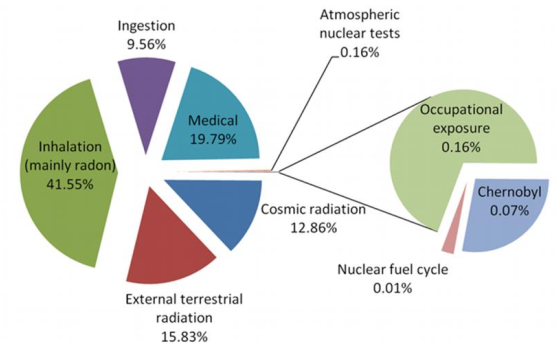
\includegraphics[scale=0.5]{2Introduction/RadioactiveDosePopulation.png}
\centering
\caption{Annual average distribution of the radioactive dose received by the population~\cite{IAEA}\label{fig:RadioactiveDosePopulation}.}
\end{figure}

\begin{table}[h]
\centering{}%
\begin{tabular}{lcc}
\toprule 
Radiation source & Eff. dose ($\milli\sievert/$yr) & Typical range ($\milli\sievert/$yr)\tabularnewline
\midrule
\midrule 
Cosmic (external) & $0.39$ & $0.3 - 1.0$ \tabularnewline
Terrestrial (external) & $0.48$ & $0.3-0.6$ \tabularnewline  
Inhalation (internal) & $1.26$ & $0.2-10$ \tabularnewline
Ingestion(internal) & $0.29$ & $0.2-0.8$ \tabularnewline
\midrule
Total & $2.42$ & $1-12.4$ \tabularnewline
\bottomrule
\end{tabular}
\caption{Annual average distribution of the effective dose received by the population due to natural radioactivity~\cite{UNSCEAR, CSN}.}
\label{tab:RadioactiveNaturalDosePopulation}
\end{table}

Since the discovery of radioactivity by Henri Becquerel in $1896$, lots of nuclear-based technologies were developed and applied to various fields such as Energy, Chemistry, Biology, Technology, Medicine, Industry, etc. Due to nuclear applications, a number of anthropogenic radioactive sources have emerged in society, resulting in radioactive elements released into the environment. It can be noticed in Figure \ref{fig:RadioactiveDosePopulation} that the most important part of the dose received by the population from artificial sources comes from medical practice. The growth of knowledge and the development of measurement techniques for radioactivity have provided evidence of the harmful effects of radioactivity on living organisms. This leads to the necessity of controlling the radiation to which the population is exposed, keeping it under safe limits. To accomplish this purpose, several organizations were created to propose recommendations for radiological protection to the different state organisms and governments at the international level. The main ones are:

\begin{enumerate}
\item{} The International Commission of Radiological Units and Measurements (ICRU) \cite{ICRU}, created during the first International Conference of Radiology held in London in 1925 to define concepts and units necessary to quantify the negative effects of radioactivity.

\item{} The International Commission on Radiological Protection (ICRP) \cite{ICRP}, created in 1928 by the International Society of Radiology (ISR) \cite{ISR}. The ICRP aims to make recommendations and provide guidance on different aspects of protection against radioactivity. The ICRP does not have the legal capacity to enforce its recommendations, but these are widely included in the legislation of most countries. %is fairly consistent with them.

\item{} The United Nations Scientific Committee on the Effects of Atomic Radiation (UNSCEAR) \cite{UNSCEAR}, created in 1955 with the goal of estimating and reporting the levels and effects of ionizing radiation on the population and the environment. These estimates are taken into account by governments worldwide to establish their safety standards.

\item{} The International Atomic Energy Agency (IAEA) \cite{IAEA}, created in 1957 to promote the peaceful use of nuclear energy and to avoid its use for military purposes such as nuclear weapons. Although established independently from the United Nations through its international treaty, the IAEA reports regularly to both the United Nations and the Security Council.

\item{} The European Atomic Energy Community (EURATOM), created in 1957, which is an international organization ruled by the EURATOM treaty. Its objective is to coordinate research programs for the peaceful use of nuclear energy and the sharing of knowledge, infrastructures and funding of nuclear energy.

\item{} The Nuclear Safety Council (CSN) \cite{CSN} of Spain, created in 1980, is the authority in Spain for nuclear safety and radiation protection. It has the objective of protecting employees, the general population and the environment from the harmful effects of ionizing radiation from anthropogenic origin. For this goal, the CSN ensures that nuclear and radioactive facilities are operated safely and establishes the preventive and corrective measures to be applied in radiological emergencies. The CSN manages two detector networks to control the levels of radioactivity in the environment and to assess the impact of radioactive facilities:

\begin{enumerate}
\item{} The network of automatic stations REA (Red de Estaciones Automáticas) \cite{REA}. The REA consists of several gamma detectors, distributed across the country as indicated in Figure \ref{subfig:REA}, which measure the radioactive dose in real time. The REA is employed for real-time detection of radiological issues to enable taking prompt safety measures.

\item{} The network of sampling stations REM (Red de Estaciones de Muestreo) \cite{REM}. The REM consists of a collection of points, shown in Figure \ref{subfig:REM}, from which samples are taken and measured in a laboratory. About twenty Spanish laboratories integrate this network. The objective of the REM is to characterize the concentration and evolution of radioisotopes present in the radioactive background of Spain and to quantify the impact of radioactive facilities on the environment.
\end{enumerate}

\begin{figure}
\centering
    \begin{subfigure}[b]{0.7\textwidth}
    \centering
    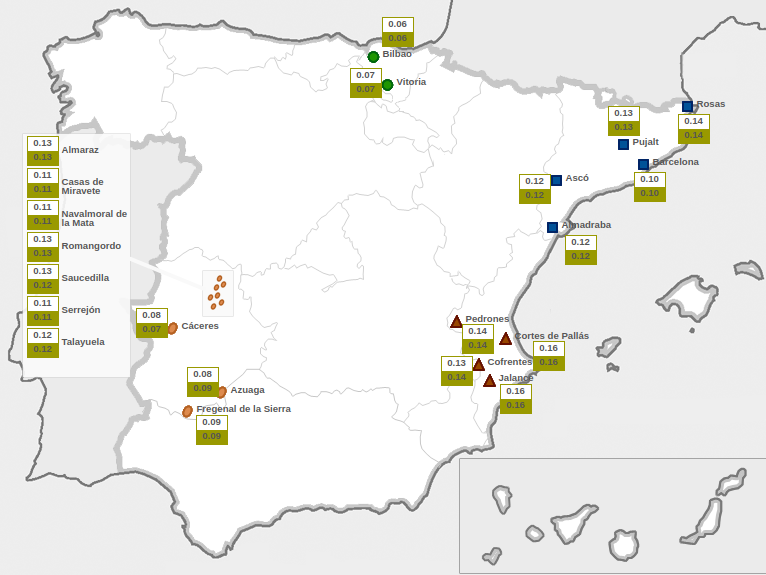
\includegraphics[width=\textwidth]{2Introduction/REA.png}  
        \caption{}\label{subfig:REA}
    \end{subfigure}
    \hfill
    \begin{subfigure}[b]{0.7\textwidth}
    \centering
    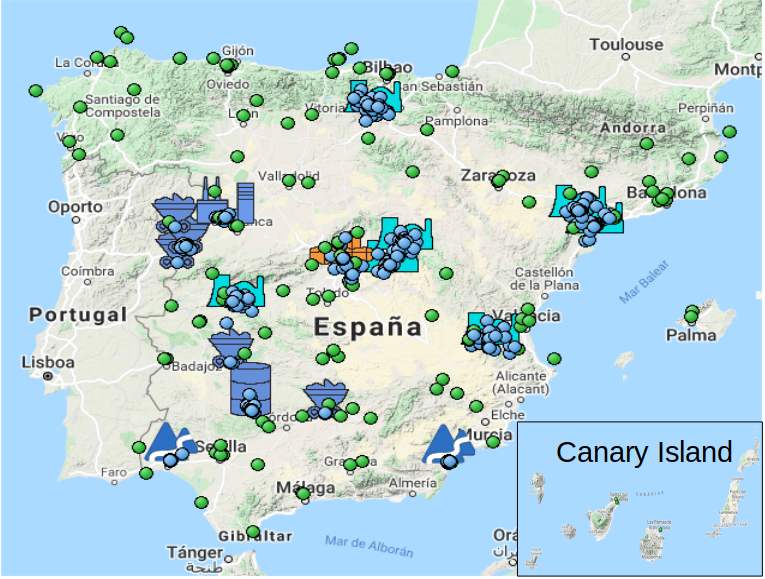
\includegraphics[width=\textwidth]{2Introduction/REM.png}  
    \caption{\label{subfig:REM}}
    \end{subfigure}
 \caption{Networks of automatic and sampling stations managed by the Spanish CSN. a) Measurement locations of the REA \cite{REA}. The white and green insets are the daily and monthly average of the gamma dose, respectively. b) Measurement locations of the REM \cite{REM}. Blue dots are locations near nuclear facilities, and green dots are locations uniformly distributed throughout the country.}
 \label{fig:NetworksCSN}
\end{figure}
%There are other networks that measure different parameters such as the concentration of $\ce{^{222}Ra}$ in the air. The measurements of all the networks complies with to the EUROTAM treaty \cite{100BqL}.

\end{enumerate}

The goal of the TRITIUM project is to develop a monitor capable of automatically measuring low levels of tritium in water in quasi-real-time\footnote{Quasi-real-time is an approximation of real-time measurements. It means a relatively small time, like less than $1~\hour$.}. This monitor is intended to be included in the REA.

Tritium is one of the radioactive isotopes routinely measured in REM tests. It is detected through the low-energy electrons produced in its beta decay, mainly using the Liquid Scintillation Counter technique (LSC). Due to the limitations of the current tritium detection techniques, described in section \ref{sec:StateOfTheArt}, the TRITIUM project was recently proposed with the objective of building a tritium detector based on scintillating fibres in contact with the water sample. The photons produced in these scintillating fibres are read out by photosensors, either photomultiplier tubes (PMTs) or silicon photomultipliers (SiPMs). The final emplacement of the TRITIUM monitor is a site close to the Arrocampo dam (Extremadura, Spain), whose water is used for the cooling system of the Almaraz nuclear power plant (NPP), located 4 km upstream from the Arrocampo dam. The monitor will be used to ensure that the tritium levels of the Arrocampo dam  water are below the legal limit of $100~\becquerel/\liter$ specified in the EURATOM Directive 2013/59/Euratom \cite{100BqL}. In addition, this will confirm the correct operation of the Almaraz NPP, since an increase of tritium activity released could indicate a malfunctioning of the reactor. This monitor could also be used in many different places with radioactive facilities like the future fusion power plants\footnote{The International Thermonuclear Experimental Reactor, ITER, will need up to several tens of kilograms of tritium to function, which corresponds to several $\tera\becquerel$ of activity.}, nuclear research facilities\footnote{Tritium is one of the main emissions from nuclear research facilities \cite{FERMILAB, BrookHavenNationalLaboratory}.} or tracking the pathway of tritium discharges to groundwater \cite{TrackingTritium}. 

Tritium is one of the most abundantly produced radioisotopes in an NPP, as it was verified in the United States Department of Energy (DOE) \cite{FiberDetector1a, FiberDetector1b}, in several research facilities in China \cite{CommonEmissionTritium} and places close to them (ground, surface and wastewater). Tritium is produced in the nuclear reactor cooling water system of NPPs by neutron capture of deuterium existing in the heavy water ($\ce{D_2 O}$), semi-heavy water ($\ce{H D O}$) or deuterium created by neutron capture in light water ($\ce{H_2 O}$). Tritium is finally released partially or totally into the environment in a quantity that depends on the reactor type, as shown in Table \ref{tab:TritiumEmisionsNPPs}. The most common form in which tritium is released into the environment is $\ce{HTO}$ \cite{CommonEmissionTritium}.
%All these processes have a large probability of happening due to the huge neutron flux, of the order of $10^{14} ~\ce{n} \, \cm^{-2} \second^{-1}$ in the nuclear reactor \cite{CrossSeccionNeutrons}

\begin{table}[htbp]
\centering{}%
\begin{tabular}{lcc}
\toprule 
Reactor type & Gaseous discharge ($\giga\becquerel/$y) & Liquid discharge ($\giga\becquerel/$y)\tabularnewline
\midrule
\midrule 
PWR & $3.70\cdot 10^{3}$ & $2.59\cdot 10^{4}$ \tabularnewline
BWR & $1.85\cdot 10^{3}$ & $3.70\cdot 10^{3}$ \tabularnewline
HWR & $7.40\cdot 10^{5}$ & $1.85\cdot 10^{5}$ \tabularnewline
GCR & $7.40\cdot 10^{3}$ & $1.11\cdot 10^{4}$ \tabularnewline
\bottomrule
\end{tabular}
\caption{Emission of tritium per year from different types of nuclear reactors: Pressurized Water Reactor (PWR), Boiling Water Reactor (BWR), Heavy Water Reactor (HWR) and Gas-Cooled Reactor (GCR) \cite{CommonEmissionTritium}.}
\label{tab:TritiumEmisionsNPPs}
\end{table}

NPPs are operational for more than 60 years and, nowadays, they are essential for providing a large part of the electric power used all over the world (more than $20\%$ in Spain \cite{PercentageEnergySpain} and more than $10\%$ in the world \cite{PercentageEnergyWorld}). Although the Spanish government is planning to progressively shut all NPPs down, there are other countries like China \cite{60ReactorsChina} or the United States \cite{35MillionsUSA} that promote their use. NPPs are a profitable investment since they are one of the cheapest sources of energy production. Their energy production rate is stable since it does not depend on meteorological conditions. Moreover, NPPs do not emit greenhouse gases. Although there are alternative energy sources which are being developed quickly (photovoltaic, wind, tidal energy, etc.), as well as other concepts of energy production and saving (local production, energy efficiency, smart cities, etc.), they are currently not enough to cover the population needs. However, NPPs have some important drawbacks such as contamination of fresh water from uranium mining, nuclear waste, nuclear proliferation and the risk of radioactive contamination from accidents as happened in the past: Chernobyl, Fukushima and Three Mile Island \cite{ThreeMileIsland}. In any case, world nuclear energy production is most likely not going to be stopped in the next decade. In fact, the United States Energy Information Administration (EIA) expects a future increase of nuclear energy production \cite{EIAOutlook}. Therefore, safety is not a negotiable aspect and there must be a development of safeguards, like alarm systems, that warn of any malfunction of NPPs. 

%which is normally done by liquid scintillation counter technic (LSC). This technic has a very good detection capability and precision but it has the inconvenient of providing a delayed results of about 1-2 days or even more. Liquid scintillation technique for the tritium measurement will be presented in section \ref{sec:StateOfTheArt}. \label{sec:Introduction}
	\newpage

	\section{Tritium properties}
	Tritium is the only radioactive isotope of hydrogen. It was first time produced in $1934$ from neutron capture of deuterium by Ernest Rutherford, Mark Oliphant and Paul Harteck \cite{TritiumDiscovery} and it was first time isolated in 1939 by Luis Walter Alvarez and Robert Cornog \cite{TritiumIsolate}, who checked that tritium is a radiactive element. 

Tritium is naturally produced in the environment through the interaction of cosmics rays and gaseous elements of the upper atmosphere like nitrogen ($\ce{^{14}N}(\ce{n},\ce{^{3}H})\ce{^{12}C}$) \cite{TritiumHandling} and oxigen ($\ce{^{16}O}(\ce{n},\ce{^{3}H})\ce{^{14}N}$) \cite{OxigenTritium}. Around 99\% of this tritium form water (\ce{HTO}) and reaches the earth's surface as rain with an estimated produccion rate of $4\cdot 10^6 ~\curie/$yr ($1.48 \cdot 10^8 ~\giga\becquerel/$yr), producing a tritium concentration of $0.6-1.2~\becquerel/\liter$ in precipitation \cite{CommonEmissionTritium, TritiumHandling}. 

Tritium can be produced artificially in the environment from different anthropogenic sources \cite{CommonEmissionTritium, TritiumHandling}. There is a large amount of tritium which was produced in military nuclear test explosions between 1945 and 1975, with an estimated total production of $8 \cdot 10^9~\curie$ ($2.96 \cdot 10^{11}~\giga\becquerel$) and a part of which remains to the date. In these nuclear explosions, tritium was produced mainly from the nuclear reactions $\ce{^{14}N}(\ce{n},\ce{^{3}H})\ce{^{12}C}$ and $\ce{^{2}H}(\ce{n},\gamma)\ce{^{3}H}$. Tritium can be also produced by commercial producers of radioluminiscent and neutron generator devices ($1 \cdot 10^6~\curie/$yr), nuclear power and defense industries (around $2 \cdot 10^6~\curie/$yr) and several research facilities and nuclear reactor for energy production ($2 \cdot 10^6 \curie/\giga\watt$yr), whose main production cross sections are shown in Table \ref{tab:NuclearReactionsTritiumProduction}: 

\begin{table}[htbp]
\begin{center}
\begin{tabular}{|c|c|c|c|}
\hline
Element & Origin & Nuclear reaction & Cross section ($\barn$)\\
\hline \hline \hline
$\ce{^{2}_{1}H}$ & Water coolant & $\ce{^{2}_{1}H}(\ce{n},\gamma)\ce{^{3}_{1}H}$ & $5.2 \cdot{} 10^{-4}$ \\ \hline
$\ce{^{3}_{2}He}$ & Helium coolant & $\ce{^{3}_{2}He}(\ce{n},\ce{p})\ce{^{3}_{1}H}$ & $5330$ \\ \hline
$\ce{^{6}_{3}Li}$ & Moderator & $\ce{^{6}_{3}Li}(\ce{n},\alpha)\ce{^{3}_{1}H}$ & $940$ \\ \hline
$\ce{^{10}_{5}B}$ & \parbox{8em}{\centering Moderator,\\ control rods} & $\ce{^{10}_{5}B}(\ce{n},2\alpha)\ce{^{3}_{1}H}$ & $3835$ \\ 
\hline
\end{tabular}
\caption{Most common nuclear reactions of artificial tritium production~\cite{CommonEmissionTritium}}
\label{tab:NuclearReactionsTritiumProduction}
\end{center}
\end{table}

%\begin{equation}
%\ce{^{2}_{1}H}(\ce{n},\gamma)\ce{^{3}_{1}H} \qquad \sigma= 5.2 \cdot{} 10^{-4}~\barn  ~~~\cite{CommonEmissionTritium}
%\label{eq:capneuH2}
%\end{equation}

%\begin{equation}
%\ce{^{3}_{2}He}(\ce{n},\ce{p})\ce{^{3}_{1}H} \qquad \sigma= 5330~\barn ~~~\cite{CommonEmissionTritium}
%\label{eq:capneuHe3}
%\end{equation}

%\begin{equation}
%\ce{^{6}_{3}Li}(\ce{n},\alpha)\ce{^{3}_{1}H} \qquad \sigma= 940~\barn ~~~\cite{CommonEmissionTritium}
%\label{eq:capneuLi6}
%\end{equation}

%%\begin{equation}
%%\ce{^{7}_{3}Li}(\ce{n},\alpha)\ce{^{3}_{1}He} + \ce{n} ~~~\cite{CommonEmissionTritium}
%%\label{capneuLi7}
%%\end{equation}

%\begin{equation}
%\ce{^{10}_{5}B}(\ce{n},2\alpha)\ce{^{3}_{1}H} \qquad \sigma= 3835~\barn ~~~\cite{CommonEmissionTritium}
%\label{eq:capneuB10}
%\end{equation}

%\begin{equation}
%\ce{^{11}_{5}B}(\ce{n},2\alpha)\ce{^{3}_{1}H} + n ~~~\cite{CommonEmissionTritium}
%\label{capneuB11}
%\end{equation}
%$\eqref{capneuLi6}$ para referenciar ecuaciones

%There are two more nuclear reaction with which we can produce tritium:

%\begin{equation}
%\ce{^{1}_1 H} (2 \cdot{} \ce{n},\ce{p})\ce{^{3}_1 H}
%\label{doblecapneuH}
%\end{equation}

%\begin{equation}
%\ce{^{2}_1 H}(\ce{n},\gamma)\ce{^{3}_1 H}
%\label{capneuD}
%\end{equation}

Tritium levels in the environment when anthropological radioactive sources are not involved are between $1$ and $4~\becquerel/\liter$. This is a higher value than the expected due to the cosmogenic background levels ($0.6-1.2~\becquerel/\liter$, previously mentioned) \cite{FranceTritiumEnvironment}. It can be explained by the consequences of nuclear weapons tests.

Tritium levels in rivers around a nuclear facility are between $1$ and $10~\becquerel/\liter$ and even between $20$ and $50~\becquerel/\liter$ at the water discharge site of NPPs \cite{FranceTritiumEnvironment}, where the produced tritium is partially or totally released into the environment, mainly in the $\ce{HTO}$ water form.

The effect of NPP on tritium levels can be observed using the public measurements of the REM, explained in the section \ref{sec:Introduction}. For example, in the case of Cofrentes, which is the closest nuclear power plant to Valencia and the one in whose measurements are involved LARAM\footnote{LARAM is a Valencia laboratory specialized in environmental radioactivity measurements}, the tritium levels in the river are measured in three different places, marked on the map shwon in Figure \ref{fig:SamplingLocations}. The first place, P1, is located in the river, $6~\kilo\meter$ upstream from the NPP, the second place, P2, is located $1~\kilo\meter$ downstream and the third place, P3, is located $5~\kilo\meter$ downstream. The level of Tritium measured in these three locations is shown over time in Figures \ref{fig:TritiumL6kB}, \ref{fig:TritiumL1kA} and \ref{fig:TritiumL5kA} respectively.

\begin{figure}[hbtp]
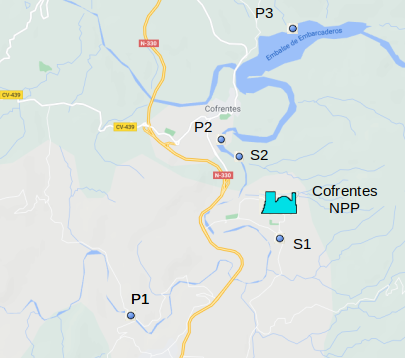
\includegraphics[scale=0.5]{2Introduction/CofrentesMaps.png}
\centering
\caption{Tritium sampling locations around Cofrentes NPP.\label{fig:SamplingLocations}}
\end{figure}

\begin{figure}[hbtp]
 \centering
  \subfloat[Tritium activity $6~\kilo\meter$ upstream.]{
  \label{fig:TritiumL6kB}
    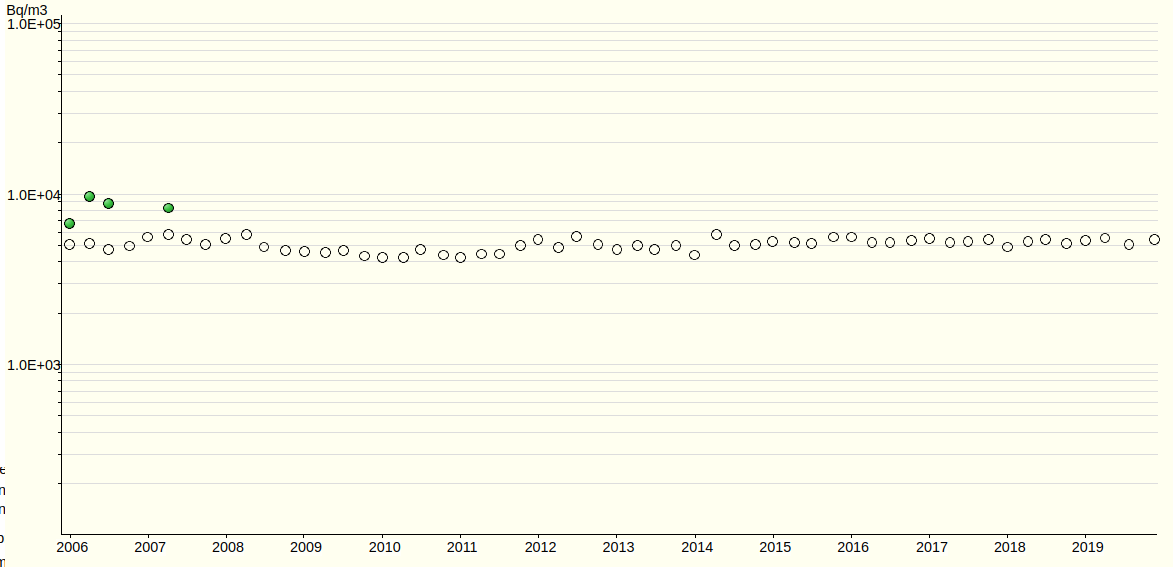
\includegraphics[width=0.47\textwidth]{2Introduction/6km_before.png}}
    %\newline
      \subfloat[Tritium activity $1~\kilo\meter$ downstream.]{
   \label{fig:TritiumL1kA}
    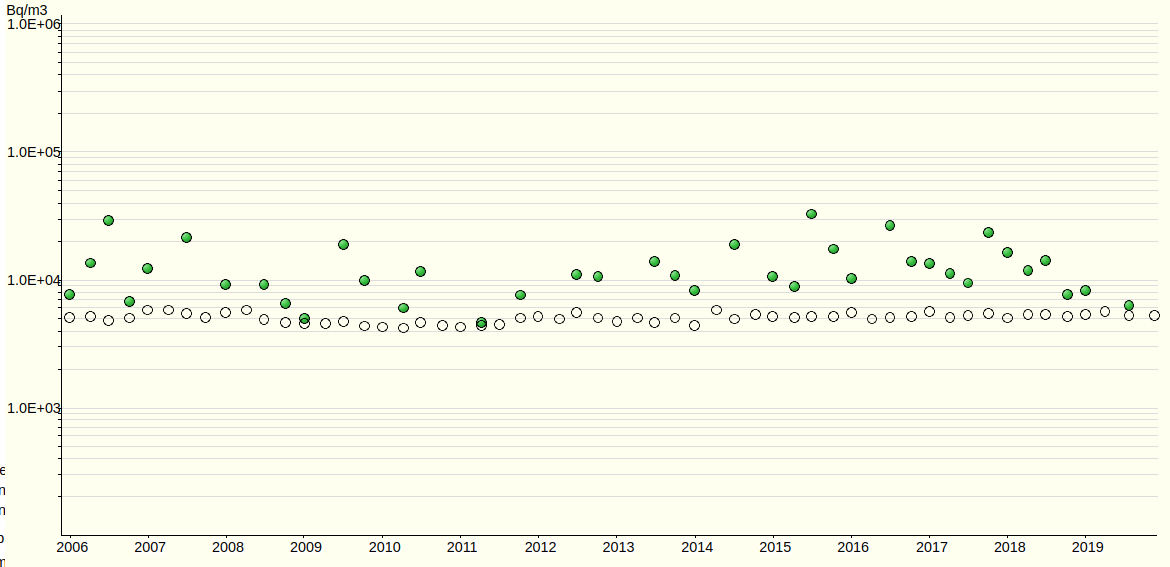
\includegraphics[width=0.47\textwidth]{2Introduction/1km_after.png}}
    \newline
  \subfloat[Tritium activity $5~\kilo\meter$ downstream.]{
  \label{fig:TritiumL5kA}
    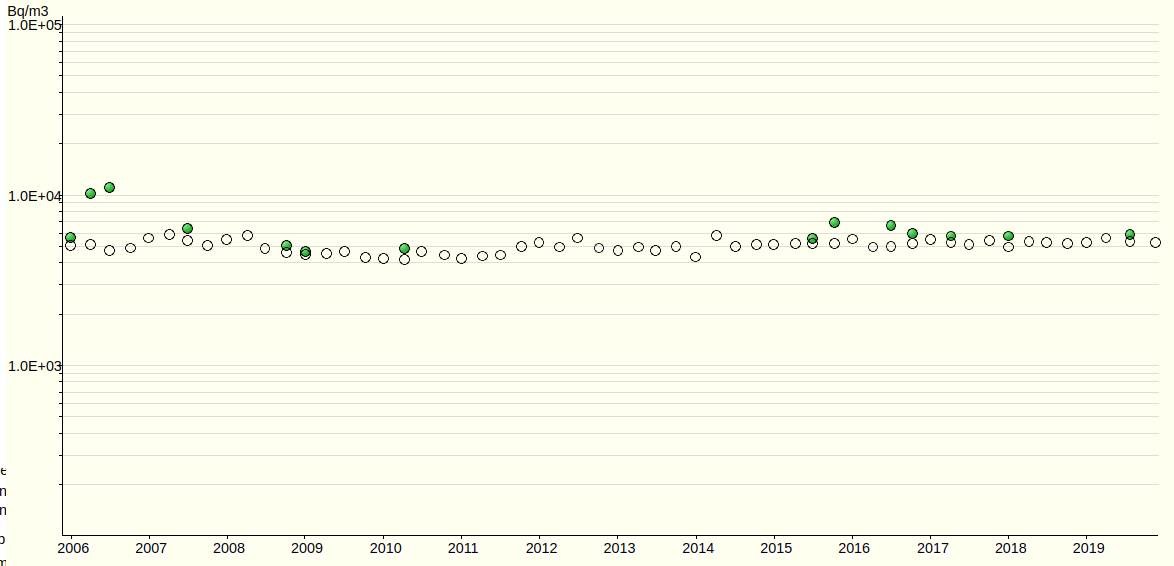
\includegraphics[width=0.47\textwidth]{2Introduction/5km_after.png}}
 \caption{Tritium activity levels in surface water around Cofrentes NPP from January $2006$ to November $2019$. The white points are used for the detection limit and the green points are used for the measured activity, when it is above the detection limit.~\cite{REM}}
 \label{fig:MeasurementsCofrentesSurface}
\end{figure}

In these figures, the detection limit and the measured activity are shown using white dots and green dots respectively. The measured activity is only displayed when it is larger than the corresponding detection limit. As it can be seen, the tritium level in the river increases due to the discharge of the NPP and it is diluted again after $4~\kilo\meter$ downstream. 

Two additional measurements of the tritium level in groundwater have been included, points S1 and S2 on the map in Figure \ref{fig:SamplingLocations}, which are located $1~\kilo\meter$ before and $1~\kilo\meter$ after the NPP. Both tritium levels are shown in the figure \ref{fig:TritiumLG1kB} and \ref{fig:TritiumLG1kA} respectively, where it can be verified that the nuclear power plant has not affected them.

\begin{figure}[hbtp]
 \centering
      \subfloat[Tritium activity $1~\kilo\meter$ before NPP.]{
   \label{fig:TritiumLG1kB}
    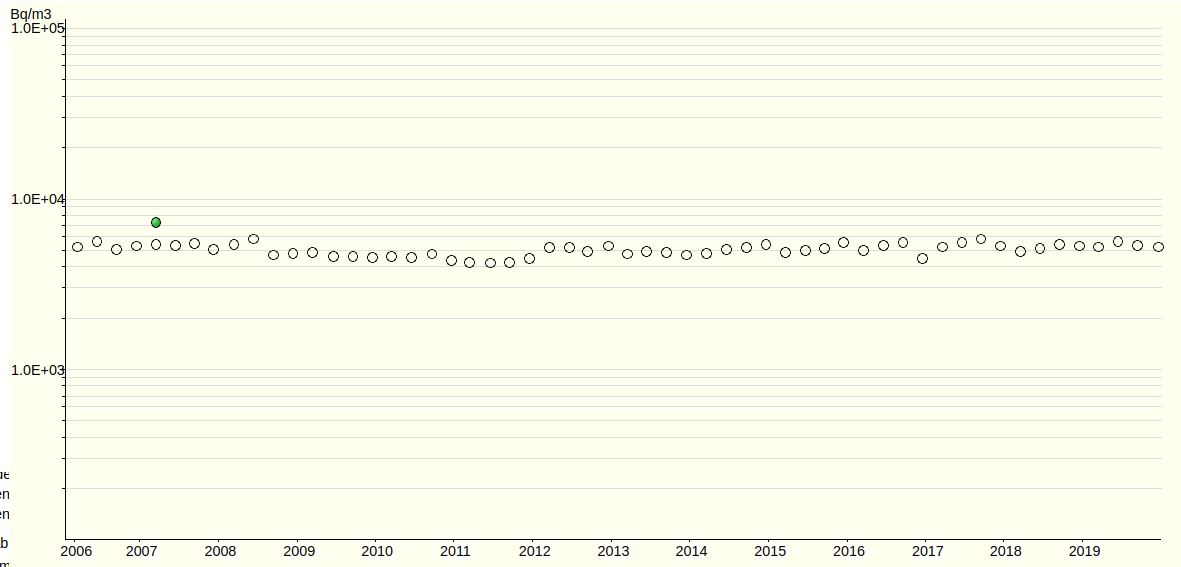
\includegraphics[width=0.47\textwidth]{2Introduction/Subterranea_before.png}}
    %\newline
  \subfloat[Tritium activity $1~\kilo\meter$ after NPP.]{
  \label{fig:TritiumLG1kA}
    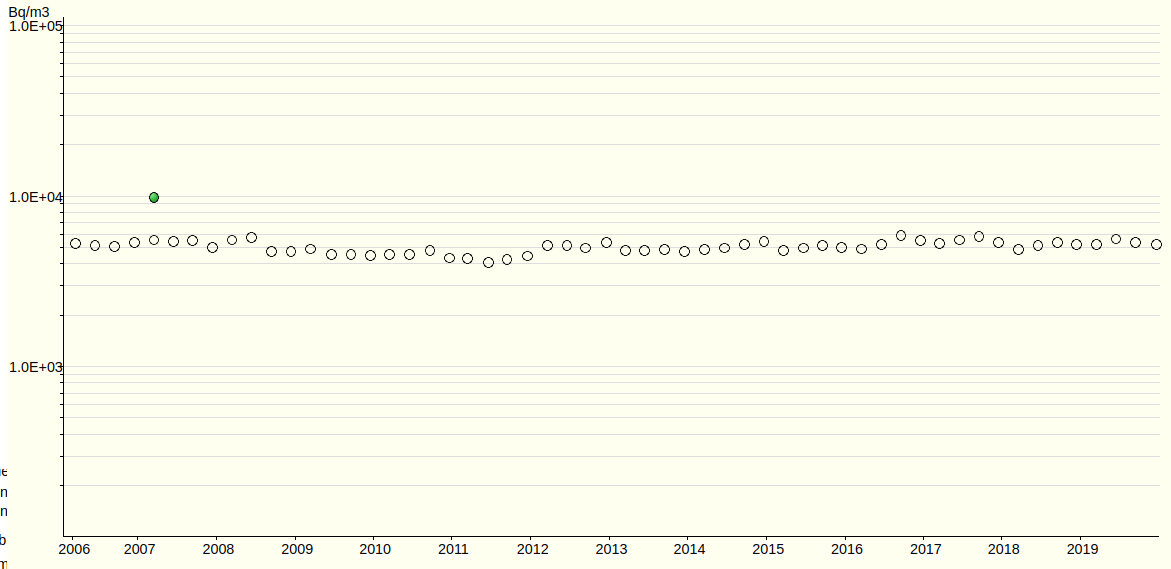
\includegraphics[width=0.47\textwidth]{2Introduction/Subterranea_1_km_later.png}}
 \caption{Tritium activity levels in groundwater around Cofrentes NPP from January $2006$ to November $2019$.~\cite{REM}}
 \label{fig:MeasurementsCofrentesGroundWater}
\end{figure}

It is important to note that, although environmental tritium levels have been affected due to NPP, these levels are below the legal limit. The maximum level of tritium measured since of January 2, 2006 is around $32~\becquerel/\liter$, below to the legal limit in Europe, $100~\becquerel/\liter$.

Tritium is a radioactive element whose half-life time is $T_{1/2}= 12.32$ years. It has one proton and two neutrons and decays exclusively through $\beta$ radiation. It decay $100\%$ directly to the ground state of Helium ($\ce{^{3}_{2}He}$), which is a stable nuclei, thorugh the decay scheme of equation \ref{eq:TritiumDecay}:

%In this decay, one neutron of tritium is transformed transformed into a proton, an electron and an electron-antineutrino, according to the following decay scheme:

%\begin{equation}
%\ce{n} \longrightarrow \ce{p}  + \ce{e^-}  + \ce{\overline{\nu}_e}
%\label{eq:BetaDecay}
%\end{equation}



\begin{equation}
\ce{^{3}_{1}H} \longrightarrow \ce{^{3}_{2}He}  + \ce{e^-}  + \ce{\overline{\nu}_e}
\label{eq:TritiumDecay}
\end{equation}

In Figure \ref{fig:TritiumDecay} the scheme of tritium energy levels is shown. In this decay it is not possible to detect the neutrino because of its extremely weak interaction with matter ($\sigma \propto 10^{-42} ~ \cm^2$ \cite{CrossSeccionNeutrino}) and, since $\ce{^{3}He}$ has a much larger mass than electrons and neutrinos, by conservation of energy and momentum, the energy that is taken by this daughter nucleus is very small. Therefore, the detection of tritium is through its decay electron. 

\begin{figure}[hbtp]
 \centering
  \subfloat[Tritium energy levels \cite{TritiumDecayEnergyLevels}]{
   \label{fig:Energy_levels}
    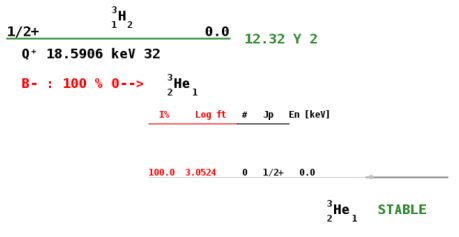
\includegraphics[width=0.60\textwidth]{2Introduction/esquema_niveles_energeticos.png}}
  \subfloat[Graphic representation of tritium decay \cite{TritiumDecayImage}]{
   \label{fig:GraphicDesintegration}
    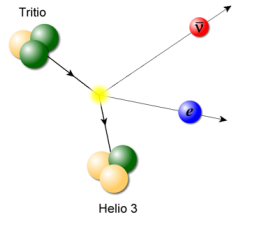
\includegraphics[width=0.40\textwidth]{2Introduction/representacion_desintegracion.png}}
 \caption{Tritium decay}
 \label{fig:TritiumDecay}
\end{figure}

The energy released in the tritium decay is $Q_\beta=18.6~\keV$, which is divided between the decay products. Therefore, the energy spectrum of the decay electrons is a continuum with a maximum value of $18,6~\keV$, as shown in Figure \ref{fig:TritiumDecaySpectrum}. This energy spectrum has an average of $5.7~\keV$ and the most likely value is slightly below, around $4.5~\keV$.

\begin{figure}[hbtp]
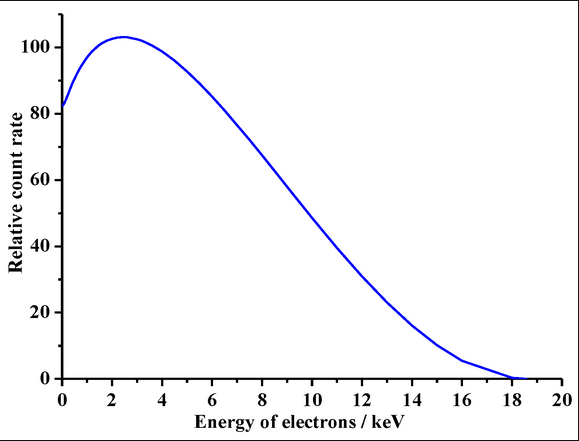
\includegraphics[scale=0.6]{2Introduction/Espectro_tritio.png}
\centering
\caption{Energy spectrum of tritium electrons ~\cite{TritiumEspectrum}\label{fig:TritiumDecaySpectrum}}
\end{figure}

%We have to keep in mind that, although the helium isotope is stable, it will be exited immediately after this decay. As a consequence, after the tritium $\beta^-$ decay, we will have a subsequent dexcitation of the $\ce{^{3}He}$ which will produce photons, $\gamma$, with several well-defined energies that correspond to their energy levels, X-rays\footnote{X-rays are photons whose wavelength are between 0.01 nm and 10 nm. They are produced by nuclear deexitation.}. It will not affect our tritium measurement because, as we will see in Section  \ref{}, the probability of detecting X-rays with the photosensor that will be used is practically negligible.

%Los rayos X son una radiación electromagnética de la misma naturaleza que las ondas de radio, las ondas de microondas, los rayos infrarrojos, la luz visible, los rayos ultravioleta y los rayos gamma. La diferencia fundamental con los rayos gamma es su origen: los rayos gamma son radiaciones de origen nuclear que se producen por la desexcitación de un nucleón de un nivel excitado a otro de menor energía y en la desintegración de isótopos radiactivos, mientras que los rayos X surgen de fenómenos extranucleares, a nivel de la órbita electrónica, fundamentalmente producidos por desaceleración de electrones. La energía de los rayos X en general se encuentra entre la radiación ultravioleta y los rayos gamma producidos naturalmente. Los rayos X son una radiación ionizante porque al interactuar con la materia produce la ionización de los átomos de la misma, es decir, origina partículas con carga (iones). 

The releasing energy of the tritium decay, is very little. In fact, it is the radioactive isotope with the lowest energy released in its $\beta$ disintegration \cite{TritiumHandling}. Consequently, the $\beta$ particle which is emitted in this tritium decay will have a very small mean free path as it is shown in Table \ref{tab:MeanFreePathTritium}.

\begin{table}[htbp]
\begin{center}
\begin{tabular}{|c|c|c|}
\hline
Material & P. Depth ($5.7~\keV$) & P. Depth ($18.6~\keV$)\\
\hline \hline \hline
$\ce{\ce{^{3}_{1}H_2}}$ & 0.26 cm & 3.2 cm \\ \hline
Air & 0.036 cm & 0.45 cm \\ \hline
\parbox{10em}{\centering Water, soft tissue\\  (solid matter whose \\  density is $1~\gram\cdot\cm^{-3}$)} & 0.42 $\mu\meter$ & 5.2 $\mu\meter$ \\ \hline
\end{tabular}
\caption{Penetration depth for decay electron of mean ($5,7~\keV$) and maximum ($18,6~\keV$) energies in different media (tritium gas and air at standard conditions of temperature ($273~\kelvin$) and preassure ($1$ atm), STP, and water)~\cite{MeanFreePathDocument}}.
\label{tab:MeanFreePathTritium}
\end{center}
\end{table}

This short mean free path is a major issue in tritium detection, as it makes more difficult the electron detection, which will require a highly sensitive detector. However, it means that the tritium electrons has a low penetration in our body and easily stopped with our clothes or laboratory gloves, resulting in a low radiological hazard of external tritium.

Nevertheless, the danger of tritium increases when it is ingested or inhaled since it can bind anywhere that hydrogen can and perform the same chemical reactions, sometimes with higher rate if the tritium concentration is high enough to catalyze the reaction. 

Tritium can be absorbed in our body in three different ways, gaseous tritium (mainly HT), tritiated water (mainly HTO) and organically bound tritium (called OBT).

The gaseous tritium, which is normally found mixed in the air, is the least important since less than a $3-5 \cdot{} 10^{-3}~\%$ is absorbed, which is insignificant \cite{TritiumHandling}. However, it can be transformed into tritiated water through the oxidation and exchange reactions shown in the chemical schemes of equations \ref{eq:OxidationExchange}, which has a more important effect on health \cite{TritiumHandling}:

\begin{equation}
\begin{split}
& Oxidation: \qquad \qquad \qquad \qquad \qquad \qquad Exchange\\
& 2\cdot{}\ce{HT} + \ce{O_2} \rightarrow 2 \cdot{} \ce{HTO} ~ \quad \qquad \qquad \qquad \ce{HT} + \ce{H_2 O} \rightarrow \ce{H_2} + \ce{HTO}\\
& 2\cdot{}\ce{T_2} + \ce{O_2} \rightarrow 2 \cdot{} \ce{T_2 O} \qquad \qquad \qquad \qquad \ce{T_2} + \ce{H_2 O} \rightarrow \ce{HT} + \ce{HTO}
\label{eq:OxidationExchange}
\end{split}
\end{equation}

Tritiated water, which is normally found in drinking water or water in food, has a larger impact since the $99\%$ of it is absorbed \cite{TritiumHandling}. In addition, its biological life time of it is around $9.5$ days ($\pm50\%$), time during which tritium will remain in our body \cite{TritiumHandling, FranceTritiumEnvironment, EstimationTritiumDosi}.

This time corresponds to the water cycle in the body and, like this, it can vary due to various external parameters such as temperature, humidity, drinking habits, etc. or reduced with the use of diuretics \cite{TritiumHandling}.

Organically bound tritium, normally found in food, generally forms a covalent bond with a carbon and and it corresponds to $5-10~\%$ of tritium absorbed in the body. Although it is absorbed in less quantity in the body than tritiated water, it can be more dangerous since it has a longer biological life time. The biological life time of this tritium type depends on the affinity of the organic molecule with the different biological tissues and it can vary from tens of days to hundreds of days (larger than the ICRP estimate) \cite{FranceTritiumEnvironment, EstimationTritiumDosi, EstimationTritiumDosiRats, EstimationTritiumDosiKangarooRats}.

There are many studies showing that tritium in living matter can cause the same effects than X-rays or $\gamma$ rays, which are mutations, tumors, cancer, genetic effects, reproductive effects, etc \cite{StraumeTritiumHazard, RytoemaaTritiumHazard}. In fact, the consequences of tritium radiation can be worse than a similar $\gamma$ radiations since its biological efficiency\footnote{The biological efficiency is used to quantify the damage produced in the living cells due to an external radiation.} is two or three times larger \cite{StraumeTritiumHazard}.

In summary, tritium is a naturally occurring radioactive element that can affect health if it is released excessively. Because of that, each country has developed a legislation, shown in section \ref{sec:Legislation}, to manage the release of tritium and ensure that these background levels are safe for health.



%Tritium has different physical properties than other natural isotopes of the hydrogen like different boiling points as shown in Table \ref{tab:BoilingPoints} or the property of self-radiolysis which only happens when radioactive elements are involved. In the case of tritium dissolved in water, it is normally found forming the $\ce{HTO}$ molecule. There, the auto-radiolysis ocurrs because the energy released in tritium decay is larger than the energy bond of oxigen and hydrogen in water molecules ($5.2~\eV$) or the ionization energy of water molecules ($12.6~\eV$) so it can break up these molecules \cite{AutoRadyolisis}. Due to the auto-radiolysis, some radicals appear in the water, increasing its corrosivity. It is a fact that we have to take into account when choosing the materials that will make up the TRITIUM detector.

%\begin{table}[htbp]
%\begin{center}
%\begin{tabular}{|l|l|l|}
%\hline
%Molecule & Boiling point (for gases) ($\kelvin$) & oxidation form\\
%\hline \hline \hline
%$\ce{H_2}$ & 20.39 & $\ce{H_2 O}$ \\ \hline
%$\ce{HD}$ & 22.14 & $\ce{HDO}$ \\ \hline
%$\ce{HT}$ & 22.92 & $\ce{HTO}$ \\ \hline
%$\ce{D_2}$ & 23.66 & $\ce{D_2 O}$ \\ \hline
%$\ce{DT}$ & 24.38 & $\ce{DTO}$ \\ \hline
%$\ce{T_2}$ & 25.04 & $\ce{T_2 O}$ \\ \hline
%\end{tabular}
%\caption{Gas molecules of hydrogen isotopes and their boiling point and oxidation form.~\cite{}}
%\label{tab:BoilingPoints}
%\end{center}
%\end{table}

%Although tritium has different physical properties it has almost the same chemical behaviour than other hydrogen isotopes. Tritium, like hydrogen, is a gas at STP forming a two-atom molecules which can be $\ce{HT}$, $\ce{DT}$ and $\ce{T_2}$. 


%Due to this chemical similarity tritiated water can perform the same chemical processes than non-radiactive water, sometimes with higher rate if the tritium concentration is high enough to catalyze the reaction. Its biological hazard comes from this chemical similarity since tritiated water is able to substitute normal water in human body. 
\label{sec:TritiumProperties}
	\newpage
	
	\section{State-of-the-art in tritium detection}
	Measurement of tritium activity is one of the systematic environmental controls that have been carried out for dozens of years around nuclear power plants during their energy production and around nuclear research facilities.

As a consequence, this measurement has been attempted with many different technologies so far in order to improve the state of the art of each time. The most researched techniques are summarized in the table \ref{tab:DifferentThecnics}.

\begin{table}[htbp]
\begin{center}
\begin{tabular}{|c|c|c|c|c|}
\hline
 & LSC & IC & Calorimetry & BIXS\\
\hline \hline \hline
\parbox{5em}{\centering Measured\\ quantity} & \parbox{5em}{\centering Scintillation\\ photons} &  \parbox{5em}{\centering Ionization\\ current} & heat & X-rays\\ \hline
LDL & $\sim\becquerel$ & $10-100~\kilo\becquerel$ & $\sim~\giga\becquerel$ & $\sim~\mega\becquerel$ \\ \hline
Sample form & Liquid & Gas, vapor & All & All \\ \hline
%Disadvantages & & Gas, vapor & All & All \\ \hline
\end{tabular}
\caption{State-of-the-art in the tritium detection for different technics~\cite{TesisTritio}}
\label{tab:DifferentThecnics}
\end{center}
\end{table}

Nowadays, the most used technic for mesuring tritium in water is the LSC. It consists of mixing a liquid sample (some ml for environmental measurements or less for higher activities) with liquid scintillator. In our laboratories, LARAM, at the University of Valencia, this mixture is made in a ratio of 50:50 \cite{LSCLARAM} but it will depend on each system and each sample \cite{LSCothers} \cite{HofstetterSeveral}. In this technic, the $\beta$ energy that is emitted from the sample excites the molecular energy levels of the liquid scintillator and it is quickly desexcited emitting several photons with a well-know energy (fluorescence), normally in the visible range. Finally these photons are detected with photosensors, processed and analysed.

This technic has a very good detection capability and precision (LDL for tritium better than $1~\becquerel/\liter$ \cite{0.6Bq_L}) but it has some problems. On the one hand it need too time for taking a mesurment (more than $2$ days) and, on the other hand, although this sample could be non-radiactive, it contain toluene which is a toxical chemical waste so we need to follow a special protocol for removing this samplex. On top of that all these technics need special staff for sampling, chain-of-custody and lab analysis which consum economical and time resources. In order to avoid the last problem some unsuccessful efforts have been made in order to build a monitor of tritium with LSC \cite{OnlineLSC}. In any case, other problems still remain. 

The ionization chamber (IC) is based on a gas chamber (sample) which contains electrodes connected to different voltage. This electrodes recover the ionization current that is produced due to the $\beta$ radiation. It is a simple and fast system, but the problem is that on the one hand it has too high LDL, more than $ 10~\kilo\becquerel$, and, on the other hand, it needs the state of the sample to be gas or steam \cite{IonizationChamber1} \cite{IonizationChamber2}.

The calorimetry is based on the measurement of the heat generated due to the tritium radiation \cite{Calorimeter1} \cite{Calorimeter2}. The problem with this technic is that it has a too high LDL, of the order of $\giga\becquerel$, and it needs too long time, more than 2 days, for taking a measurement.

The Beta Induced X-ray Spectrometry (BIXS) is based on the measurement of the bremsstrahlung with PMTs of \ce{NaI} \cite{XRays1} \cite{XRays2} or with Silicon Drift Detector (SDD) \cite{Bremstrahlung} produced due to the tritium radiation. The problem with this technic is that it has too high LDL, of the order of $\mega\becquerel$.

There are many more different methods for tritium detection, although they are less used or less experimentally developed, each one with their own problems for our objective. For example,  APD \cite{APD}, which we cannot use in our case because they cannot function in contact with water, the mass spectrometry \cite{Spectrometry}, which needs to store the sample several months before taking the measurement or Cavity ring spectroscopy \cite{Ring}, which requires a special optical configuration that is not possible outside the laboratory.

We have to keep in mind that all these techniques are offline methods that take too long to finish the process of taking measurements which include sample taking, sending the sample to the lab, analyzing of the sample so we cannot use them for tritium monitoring. LSC is the only technic which has a LDL enough low to verify the compliance with the established limit, $100~\becquerel/\liter$. Therefore we will explore this area but, in order to avoid the problems related with this technic (off-line results, no-reusable liquid scintillator and the chemical toxic wastes) we will delve in solid scintillators. There are several studies that have been done so far which intend to do the same as we want with this project, to create a quasi-real time monitor of low tritium activities in water based on solid scintillation:

\begin{itemize}

\item{} First study was done by M. Muramatsu, A. Koyano and N. Tokunaga in 1967 who used a scintillator plate read out by two PMTs in coincidence \cite{Muramatsu}.

\item{} The second study was carried out by the A. A. Moghissi, H. L. Kelley, C. R. Phillips and J. E. Regnier in 1969 that used one hundred plastic fibers coated with anthracene powder and read out by two PMTs in coincidence \cite{Moghissi}.

\item{} Third study was performed by R. V. Osborne in 1969 who used sixty scintillator plates stacked read out by two PMTs in coincidences \cite{Osborne}.

\item{} Fourth study was done by the A. N. Singh, M. Ratnakaran and K. G. Vohra in 1985, who used a scintillator sponge read out by electronic coincidence \cite{Ratnakaran}\cite{Ratnakaran2000}.

\item{} Fifth study was carried out by K. J. Hofstetter and H. T. Wilson in 1991, who did different experiments for testing different shapes of scintillator plastic like several sizes of beads, fibers, etc. The better result which Hofstetter got for solid plastic scintillator was a efficiency of the order of $10^{-3}$ \cite{Hofstetter1}\cite{Hofstetter2}.

\end{itemize}

\begin{table}[htbp]
\begin{center}
\begin{tabular}{|c|c|c|c|c|}
\hline
 & \parbox{6em}{\centering Efficiency, $\eta_{det}$\\ $(cps/(\kilo\becquerel/\liter))$}  & \parbox{5em}{\centering Surface\\ $F_{sci}$ ($\cm^2$)}  & \parbox{5em}{\centering Specific efficiency\\ $\varepsilon_{det}=\eta_{det}/F_{sci}$} & LDL ($\kilo\becquerel/\liter$)\\
\hline \hline \hline
Muramatsu & $3.85 \cdot 10^{-4}$ & $123$ & $3.13 \cdot 10^{-6}$ & $370$ \\ \hline
Moghissi & $4.5 \cdot 10^{-3}$ & $>424.1$ & $<1.06 \cdot 10^{-5}$ & $37$ \\ \hline
Osborne & $0.012$ & $3000$ & $4 \cdot 10^{-6}$ & $37$ \\ \hline
Singh & $0.041$ & $3000$ & $1.37 \cdot 10^{-5}$ & $<37$ \\ \hline
Hofstetter & $2.22 \cdot 10^{-3}$ & $\sim~100$ & $<2.22 \cdot 10^{-5}$ & $25$ \\ \hline
\end{tabular}
\caption{Results of different scintillator detector for tritium detection~\cite{TesisTritio}}
\label{tab:PlasticScinTritium}
\end{center}
\end{table}

%COMPROBAR QUE ESTAN BIEN TODOS LOS DATOS (sobretodo areas, lo otro esta comprobado. A lo mejor puedo calcular el area del ultimo caso)

The results of these experiments are sumarized in the table \ref{tab:PlasticScinTritium}. We can see in the first column that the intrinsic detector efficiency, $\eta_{det}$, is very different in these experiences. As we know that, in this type of detectors, one of the most important factor, which affect to the efficiency, is the active surface of the plastic scintillator, $F_{sci}$, and we can see in the second column that it is very different en each detector, we use the specific detector efficiency (third column), in order to compare these experiments, that's, the intrinsic detector efficiency normalized to this active surface. Now we can check that, effectively, these specific efficiencies are quite similar. On top of that we can check that the better specific efficiency was obtained for Moghissi who used scintillating fibers. This is a good point which justify our choice about using of fibers like a scintillator. Finally we can see in the last column that the LDL in all these experience are more or less similar and, they are too high for our aim so developing a detector which overcome these LDL is an essential study right now in order to monitoring the tritium levels. \label{sec:StateOfTheArt}
	\newpage
	
	\section{Tritium project and Tritium monitor}
	As we have seen in the section \ref{sec:StateOfTheArt}, the current technics which exist nowadays have either higher LDL than the limit established by Council Directive, $100~\becquerel/\liter$, or they are a off-line method (too slow) so those methods cannot be used for tritium monitoring in quasi-real time. 

As a result of these limitations appear the \textit{Tritium} project \cite{TRITIUM}, whose title is "Design, construction and commissioning of automatic stations for quasi-real time monitoring of low radioactive levels of tritium in water".

This project has been funded by Interreg Sudoe program of the EEC in the 2016 call with the reference number SOE1/P4/EO214. The purpose of this project is the development of a tritium monitor in quasi-real time. This monitor consists of a ultrapure water system, which prepare the sample before we introduce it in our detector, the tritium detector where the tritium measure will be done, the active veto and the pasive shielding which reduce the natural background of our tritium detector and several types of electronic which control all these parts of the monitor, analyze the tritium measurement and will send an alarm if the limit of $100~\becquerel/\liter$ is overcome.

The tritium detector is based on measurements of low energy beta radiation from the radioactive decay of tritium. For doing this task this detector consists of scintillator fibers, that we put directly in contact with water which can contain tritium. We need to put both, scintillator fibers and tritium water, in contact due to such a low mean free path of tritium electrons (table \ref{tab:MeanFreePathTritium} of the section \ref{sec:TritiumProperties}). Then, the photons produced on this fibers will be read out by several photosensors. The photosensors which we have tested in this experiment are photoelectron multiplier tubes (PMT) and silicon photoelectron multiplier (SiPM) arrays. 

The difficulty when we try to measure tritium is to distinguish these signals from the background. This is because tritium signals are small since tritium events has low energy ($\sim~\keV$) and this is the energy range in the spectrum where there are more background counts (the lower energy in the spectrum, the more electronic noise). We will use coincidence techniques in order to reduce the counts from the background.

It is important to check the water tightness of each prototype because if the water reaches the photosensor it will be irreparably damaged. On top of that if we use high concentrations of tritium in water for laboratory tests we can contaminate this laboratory, which could be dangerous for the healthy of the workers and it could spoil measurements of future experiments.

Finally this monitor will be installed in the Arrocampo dam, Almaraz, Spain, where the Almaraz nuclear power plant release the water which is used in their cooling system, Figure \ref{fig:Arrocampo}. This NPP has two nuclear reactors whose type is PWR. This dam is located near the Tajus river, which is the largest river in Spain, $1007~\kilo\meter$. This river cross from Aragon (Spain) to Lisbon (Portugal) and flows into the atlantic ocean. This river is used for an important quantity of animals, plants and even humans because the water of this river is used as drinking water by the spanish and portuguese people. Therefore the international cooperation in order to maintain the quality of this water is very important.

\begin{figure}[hbtp]
 \centering
  \subfloat[Arrocampo dam and Almaraz Nuclear Power Plant]{
   \label{fig:Arrocampo_Dam}
    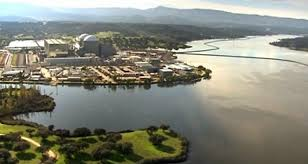
\includegraphics[width=0.47\textwidth]{2Introduction/ArrocampoDam.jpeg}}
  \subfloat[Tajus river along Spain and Portugal]{
   \label{fig:TajusRiver}
    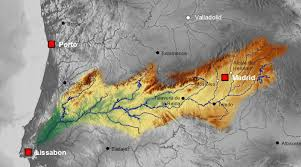
\includegraphics[width=0.53\textwidth]{2Introduction/RioTajo.jpeg}}
 \caption{Arrocampo dam, Almaraz NPP and Tajus river}
 \label{fig:Arrocampo}
\end{figure}

The \textit{Tritium} collaboration is a international group consisting of a consortium of 6 different southwestern european institution of 3 different countries: The University of Aveiro, in Portugal, The University of Bordeaux and the CNRS  (Section Aquitaine-Limousin), in France and the University of Extremadura, \textit{Junta de Extremadura} and University of Valencia, in Spain.

FOTOOS PERSONAS TRITIUM

Each institution has focused in the development of a different part of all this project:
\begin{itemize}
\item{} First, the Extremadura group has developed and installed the ultrapure water system with wich we get water with very low conductivity, $\sigma \approx 10 ~\mu S / \cm$. The conductivity of the water before the cleaning proces is around $ 1000 ~\mu S / \cm$. This clean process is very important for two reasons. On the one hand, it is important for maintaining our detector very clean, which is a critical point. On the other hand, it's important because with this process we reduce the natural background since we remove several natural radiactive isotopes that there are in this water (except tritium) such as $\ce{^{222}Rn}$, $\ce{^{40}K}$ or $\ce{^{137}Cs}$. This system will be explained in the section \ref{sec:UltraPureWaterSystem}.

\item{} Second, french group has develop the pasive shielding where our detector will work inside. It is based in ultra radiopure lead with very low intrinsic activity. The objective of this pasive shielding is to reduce the external natural background that affect to our system, for this reason we use lead. Obviously, this shielding doesn't have to affect to the measurement of our system, for this reason we use radiopure elements with very low intrinsic activity. This shielding will be explained in the section \ref{subsec:SetUpPassiveShield}.

\item{} Third, The Portugal and Spain people has collaborated for designing, developing and building four different prototypes of tritium detector and active vetos for removing cosmic events. These prototypes and vetos will be explained in the chapter \ref{chap:Prototypes} and section \ref{sec:BackgroundShields} respectively.

\item{} Lastly, The Portugal and Spanish people has also developed the simulations about this system. The program which we have used in this project is GEANT 4, which is a simulation package. It consiste in a extensive C++ library with which we can design the geometry of our detector, the physical processes which happen there, etc. This simulation will be explained in the chapter \ref{chap:Simulations}.

\end{itemize}

The tritium level which we want to mesure follow the ALARA principle (As Low As Possible Achievable) and to get it there are important characteristics which our tritium detector must have:

\begin{itemize}

\item{} \textit{Compact}. This is important because in the place where this detector will be installed the useful space that we can use is finite.

\item{} \textit{Thin active volume and large active area}. On the one hand, we have to take into account that, as we have seen in the table \ref{tab:MeanFreePathTritium} of the section \ref{sec:TritiumProperties}, the mean free path of the $\beta$ particle of tritium decay is very low so we need to work with thin active volumes. In the practice, Active thickness beyond the mean free path of the tritium will only contribute to the background. On the other hand, as we have checked in the section \ref{sec:StateOfTheArt} the efficiency of this type of detector scales with the active area so we need to design our detector with the largest possible active area.

\item{} \textit{High sensitivity to tritium}. We are going to work with low tritium activities so we need to reduce as much as possible the non-detected tritium events.

\item{} \textit{High specificity to tritium}. We need that our detector is able to distinguish the tritium signal of the signal of other radiactive elements which can be present in the initial sample.

\item{} \textit{Quasi-real time response}. As we have seen it is important that our sistem can work in quasi-real time in order to detect any problem as fast as possible. 

\item{} \textit{Rugged system}. Finally, we have to take into account that our objective will be installing an automatical system which will work during a lot of years without specialized people so we need that our monitor are rugged. 

\end{itemize}

In order to get the measurement in quasi-real time we need to work \textit{in situ}, that's, we need that our detector is able to work in the same place that we take the sample. Whit the work \textit{in site} we achieve:

\begin{itemize}
\item{} a faster monitor because we eliminates the process of taking the sample, the chain-of-custody until this sample arrive to this laboratory and the complexity which involve these tasks. 

\item{} a better monitor since if we can work \textit{in site}, our measurements can be more frequent hence we will can identify cahnges in the activity earlier.

\item{} a cheaper monitor because we have not only the material costs attached to the sample collection, chain-of-custody of this sample, shipping of this sample to the laboratory, etc. but we have also eliminated the costs attached to the specialized staff who are involving in these tasks. Our detector will only need frequent calibrations each time in order to ensure its correct operation.

\item{} a safer monitor since the personal exposure dose is reduced and the changes in activity are detected fastly. On top of that we remove the possibles mistakes which can be done by specialized staff.

\end{itemize} \label{sec:TritiumProject}
	\newpage
	
	\section{Work scheme}
	%Tesis de fibras BCF-12

This thesis is build up as follow:...



The objetive of this three-phase project was design, develop and instalation and commisioning a automatical system capable of detection tritium which we find in the water that is used by the nuclear power plants for their cooling system. The initial idea was quantifying its activity in quasi-real time before discharging it into public rivers or seas. 

We are speaking all the time about getting the measurement in quasi-real time, that is, in less of 10 minuts but what about the real time? It is obviously imposible because we are mesuring the activity, I mean, we are counting tritium decays in samples with low activities (supposedly less than $100~\becquerel/\liter$) so we need some time in order to get enough stadistic with which we can distinguish the tritium signal to the background in our system.

In order to get the measurement in quasi-real time we need to work \textit{in situ}, that's, we need that our detector is able to work in the same place that we take the sample. The reason of this fact is because if we need to move the sample we lose a lot of time (1 or 2 days in some cases). Furthermore if we avoid to move the samples we get a:

\begin{itemize}
\item{} faster detector because we eliminates the process of taking the sample, the chain-of-custody until this sample arrive to this laboratory and the complexity which involve these tasks. 

\item{} better detector since if we can work \textit{in site}, our measurements can be more frequent hence we will can identify cahnges in the activity earlier.

\item{} cheaper detector because we have removed all the cost associated with the sample collection, chain-of-custody of this sample, shipping of this sample to the laboratory and analysis thereof there. Not only we have eliminated the material costs attached to this tasks (material, transport, etc) but we have also eliminated the costs attached to the specialized staff who are involving in these tasks. With our detector we will only need frequent calibrations each time, which we consider suitable, in order to ensure the correct operation of this detector

\item{} safer detector since the personal exposure dose is reduced and the changes in activity are detected fastly. On top of that we remove the possibles mistakes which can be done by specialized staff who follow each protocol of this tasks.

\end{itemize} 

Dividiremos este trabajo en seis partes:
\begin{enumerate}
\item{} En primer lugar, se realizará un estudio sobre las fibras centelleadoras para  determinar  el protocolo de manipulación para obtener un  procedimiento de preparación de  un haz de fibras centelleadoras con un buen rendimiento óptico. 

\item{} En segundo, lugar estudiaremos el procedimiento de calibración de los SiPM,  fundamental para el experimento.  No se necesita realizar una calibración de los PMT, paso igualmente importante al anterior, ya que este trabajo fue realizado recientemente por otro componente del grupo.

\item{} En tercer lugar, se describirá  el primer prototipo diseñado, formado por un haz de 35 fibras centelleadoras sin clad leídas por PMT,  incluyendo el protocolo del proceso de llenado con agua tritiada que tuvo que ser desarrollado para cumplir los requisitos de protección radiológica y evitar contaminación accidental,  y los  resultados obtenidos con el mismo.

\item{} En cuarto lugar, se presentarán las simulaciones realizadas con el programa de Geant4 en una configuración sencilla.

\item{} En quinto lugar, se expondrán aspectos a estudiar en el futuro inmediato y en etapas posteriores, durante la Tesis Doctoral. 


\item{} Se presentarán, finalmente, los resultados, logros y conclusiones alcanzadas en el desarrollo del  trabajo.

\end{enumerate}

For process monitoring purposes it is needed to know how much tritium is in
the processed water, which is done mostly by offline methods, also involving handling
of tritiated water by the operating personnel. Since tritiated water is highly toxic, it
would be advantageous to have an online and inline monitor, which eliminates the need
of sample taking and also speeds up the measurement process.
In this thesis the investigation of a plastic scintillator-based tritium detector is
presented. The main goal was to test the concept for higher concentrations as before
(up to several GBq/l concentration) and investigate possible enhancements of the scin-
tillator geometry, besides understanding the detection process. For these purposes an
experimental setup consisting of standard industrial parts was designed, constructed and
calibrated for HTO. Several sample chamber geometries were tested (e.g. more scintil-
lator plates above each other, varying sample volume, etc.), and the configurations were
compared in terms of sensitivity and detected pulse height spectrum. To understand the
detection process in detail, a simulation was coded and compared with the experimen-
tally obtained results.
The thesis is built up as follows: First, a brief chapter introduces tritiated water,
concerning properties and processing in tritium handling facilities. The next chapter
presents the scintillation counting method in detail, based on the available literature.
This is followed by the discussion of the previous studies in the topic of tritiated water
activity measurement, then the goals of this study are defined. Chapter 4 deals with
the design considerations and the technical details of the experimental setup. The next
chapter presents the optimization of the setup for measurement, then the calibration of
for tritium is presented. The chapter also includes the analysis of the pulse height spec-
trum of tritiated water, and results of the measurements with varying sample amount
and scintillator surface, all followed by discussion. Chapter 6 first presents the technical
improvements done on the setup, then the results of additional measurement series and
their discussion follow. In the last chapter, the simulation of the detection process is pre-
sented, together with discussion of the results. The experimentally obtained spectrum is
compared with the simulation and the implications of the differences is discussed. This
chapter is followed by a summary of the thesis, together with the conclusions drawn
from the results.\label{sec:WorkScheme}
	\newpage	
	
\chapter[Design principles]{Design principles of the Tritium monitor}\label{chap:DesignPrinciples}
	\section{Detector system overview}
	Dar una visión general del detector. Objetivo, partes, para que sirven y donde hablaré de ellas y algo para cerrar el apartado como el objetivo final más preciso.

Reescribir la siguiente sección:
This Chapter is divided in three different sections. First of all, I speak about the theoretical foundations that govern the interaction between radiation and matter. Later, I do a theoretical explanation of the behavior of a scintillator detector and their components, plastic scintillator, specifying on plastic scintillating fibers, photosensors, specifying on PMTs and SiPMs, and electronic system. Finally, I show the main parts of the TRITIUM monitor and why each of these parts is necessary. I will delve into each part in future chapters. \label{sec:MonitorOverview}
	\newpage
	
	\section{Tritium detector}
	Due to the reasons which we have discussed in the section \ref{sec:StateOfTheArt}, the type of the detector which we have developed in order to measure the tritium that there is in water samples is a scintillator detector. It consists in a chain of three main elements:

\begin{itemize}

\item{} The scintillator, that is the material in charge of detecting the tritium event. The tritium particle or a general particle (ionizing radiation) hit this material and deposits part of their kinetic energy (or all, as in the case of the tritium event) in it through ionization and excitation. Part of this energy deposited is converted in photons, generally in the visible range.

The number of photons produced carry information about the particle detected, such as its energy, type, etc.

\item{} The photosensor, which is the part of the detector in charge of detecting the photons produced by the scintillator that reach its sensitive element (the more scintillated photons arrive to your photosensor, the better signal you have in your detector). 

The most used photosensor in nuclear physics are SiPMs and PMTs which detects some of the photons produced in the scintillator and transforms it in electrons which are multiplied with a factor of around $10^6$. This millions of electrons form a electronic pulse whose properties has information of the photons that has been detected.

\item{} The electronic system, which is the part of the scintillator detector in charge of processesing and analyzing (first analogically and then digitally) this electrical pulse of the photosensor to give us useful information about the event detected that we can understand and interpret such as a number, for instance the activity, or some kind of spectrum like energy spectrum.

\end{itemize}

In figure \ref{fig:ScintillatorDetector} we can see the scheme of a scintillation detector where the scintillator material detects ionizing radiation and produces photons that will be guided by the reflector and the light guide to the photosensor. There, some of the photons that reach the sensible part of the photosensors will be converted and multiplied into millions of electrons that will form a electronic pulse. The output signal of the photosensor (electronic pulse) will be processed and analyzed by the corresponding electronics:

\begin{figure}[hbtp]
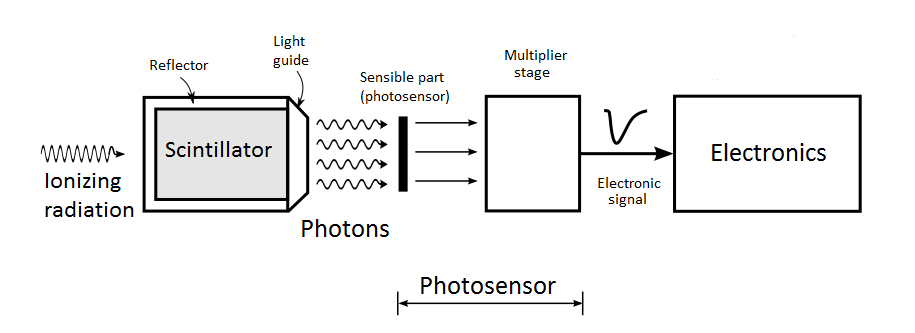
\includegraphics[scale=0.6]{3DesignPrinciples/32Tritium_detector/ScintillatorDetector.png}
\centering
\caption{Scheme of the scintillator detector \cite{CentelleadoresEspanyol}\label{fig:ScintillatorDetector}}
\end{figure}
 \label{sec:TritiumDectectorIntro}
	\newpage
	
		\subsection[Interaction of particles with matter]{Interaction of fast electrons and photons with matter}
		In this section, the explanation will only focus on the particles and energy range that are interesting for this thesis, which are electrons ($0-18~\keV$) and photons in the visible range (approx. $380-750~\nm$).

On the one hand, electrons have charge so their interaction with matter are mainly produced with the orbital electrons that there are in that matter due to the Coulomb force. The trajectory which electrons follow is much more tortuous than other heavier particles because the mass of both interacting particles is equal, electrons. Furthermore, for the same reason, these electrons lost a significant amount of energy in each collision.

In order to speak about the total energy lost of particles in matter the specific energy loss is defined as $S=-\frac{dE}{dx}$ which expresses the energy loss suffered by the particle per unit of trajectory. In the case of electrons, this total energy loss has two main contributions, the collisions (elastic and inelastic) and radiative processes (bremsstrahlung):

\begin{equation}
\frac{dE}{dx} \approx \left(\frac{dE}{dx}\right)_{c} + \left(\frac{dE}{dx}\right)_{br} ~\cite{Knoll} \cite{Leo} \qquad  \frac{\left(\frac{dE}{dx}\right)_{br}}{\left(\frac{dE}{dx}\right)_{c}} \approx \frac{EZ}{700} ~\cite{Knoll}
\label{eq:ElectronInteraction}
\end{equation}

Where $E$ is the energy of the electron in $\MeV$ and $Z$ is the atomic number of the absorbing material. Due to this energy loss, the electrons can only penetrate a material as far as they go before losing their total kinetic energy. This distance is known as range and, in the case of tritium electrons, its value is seen in the table \ref{tab:MeanFreePathTritium}.

On the other hand, photons don't have charge. Its possible interactions with the matter are photoelectric effect, Compton effect, coherent scattering and pair production and the probability of each process depends on the energy of the photon, $E_\gamma = h\nu$, and the atomic number of the material, Z, as you can see in the figure \ref{fig:ProcessesPhotons}.

\begin{figure}[htbp]
\centering
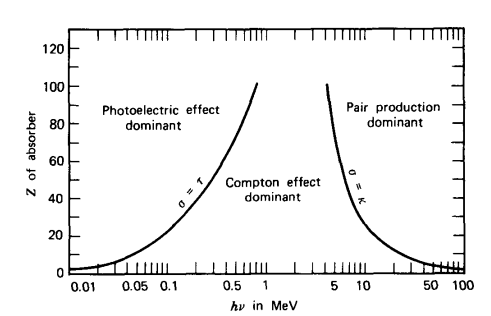
\includegraphics[scale=0.75]{3DesignPrinciples/32Tritium_detector/DominantProcessesPhotons.png}
\caption{Domain regions of the three most probable types of interactions of gamma rays with matter. The lines show the values of Z and $h\nu$ where the two neighboring effects are equally likely.\label{fig:ProcessesPhotons}~\cite{Knoll}~\cite{Leo}}
\end{figure}

We have to take into account that the only relevant photons for this thesis are in the visible range, between $400$ and $700~\nano\meter$, that corresponds with energies of the order of the $\eV$. Therefore the last effect, pair productions, will be not explained here because it needs a photon energy equal or more than $1.022~\MeV$ for happening and it is not our case.

The photoelectric effect occurs when a photon interacts with an orbital electron in the material, losing all its energy. This energy is absorbed by the electron that is released from the atom (ionization). The energy of the resulting electron, $E_e$, is:


\begin{equation}
E_e = E_\gamma - E_b ~\cite{Knoll}\cite{Leo}
\label{eq:PhotoelectricEffect}
\end{equation}

Where $E_b$ is the binding energy of the electron in this material. The probability of this effect depends on the number of available electrons through the variable Z, and the energy of the electron according to the following expression:

\begin{equation}
\left(Pr\right)_{Ph-eff} \approx \frac{Z^n}{E_\gamma^{3.5}}~\cite{Knoll}
\label{eq:PhotoelectricProb}
\end{equation}

As we can see in this expression and in the figure \ref{fig:ProcessesPhotons}, the photoelectric effect is most probably if we use elements with high atomic number. This is the reason why elements with high atomic number are the best isulators against gamma radiation and this is one of the reasons why we use lead ($Z=82$) for building our passive shielding as we will see in the section \ref{subsec:SetUpPassiveShield}. This is also the reason why elements with high atomic number are used in the cathode of PMTs. 

The Compton effect occurs when the photon interacts with an orbital electron of the material, transferring part of this energy to the electron, which is released, and this photon is scattered at an angle $\theta$ with respect to the original direction. If we neglect the binding energy, the energy transfered to this electron, $E_e$, is shown in the following equation:

\begin{equation}
E_e=\frac{\frac{E_\gamma^2}{m_oc^2}\left(1-cos\theta\right)}{1+ \frac{E_\gamma^2}{m_oc^2}\left(1-cos\theta\right)}~\cite{Knoll}\cite{Leo}
\label{eq:ComptonEffect}
\end{equation}

Where $m_0$ is the rest mass of the electron and $c$ is the speed of the light in the vacumm. The probability of the Compton effect is proporcional to the atomic number(more available electrons), Z,  and decreases with the energy of the photon. 

As we can see in the figure \ref{fig:ProcessesPhotons}, in the energies of the photons belonging to the visible range of the electromagnetic spectrum (of the order of eV), the Compton effect is only more likely in very light materials, (Z<4). For heavier materials the photoelectric effect is the dominant effect.

Finally, in the coherent scattering, the atom is neither excitation nor ionization and the photon conserve all their energy in this collision. This effect is more probably for photons with low energies and materials with high atomic numbers. Because of the fact that the energy of the photon doesn't change we will not speak more about this effect but it is important since this effect change de direction of photons and it will affect to their mean free path. \label{subsec:Interaction}
		%\newpage
					
		\subsection{Scintillators plastic} %\label{sec:Scintillators}
		The use of scintillators in radiation detection is one of the most used technics in nuclear physics. The scintillator is a material that is able to convert the kinetic energy of the incoming particles in light (photons in the visible energy range) which we can detect and quantify. It happens because the radiation excites and ionizes the scintillating atoms which, after that, are immediately de-exciting (with times of the order of picoseconds), emitting photons.

This conversion should be linear in a wide energy range of incoming particles and it is necessary that this material has good optical properties, such as being transparent to the wavelenght of their own emission and having a refractive index as close as possible to the glass for optimizing optical coupling with photosensors.

The photon emission in the scintillator is a stadistical process, which means that two exactly the same events will emmit different number of photons. It follow a poisson statistics so when we speak about the number of emmited photons we speak about the mean number of photons.

There are two types of scintillators, organics and inorganics. Inorganic scintillators normally have a higher atomic number and density so their light output are higher. Due to these reasons they are better for gamma-ray spectroscopy (take into account figure \ref{fig:ProcessesPhotons}). Organic scintillators are generally faster and they are commonly used for beta spectroscopy and neutron detection. In this seccion I focus my explanation mainly on organic scintillators since they are the ones we have used in our research. 

Organic scintillators are based on a scintillator material, which produces light, dissolved in a base solvent. This solvent is normally based on aromatic hydrocarbons (carbon atoms linked together), that is, they are mainly composed of carbon and hydrogen atoms as we can see in the molecules of some of the most widely used scintillators, $\ce{C_{18}H_{14}}$, $\ce{C_{24}H_{22}N_{2}O}$ or $\ce{C_{15}H_{11}NO}$ whose average atomic numbers are between 3,5 and 5.

The scintillator molecules, in which the organic scintillators are based, have the so called $\pi$-electron structure. The energy levels of their electrons are commonly ilustrated with a Jablonsky diagram, figure \ref{fig:JablonskyDiagram}, where we can see the fundamental single state, $S_{0i}$, where the valence electrons are, the excited single states, $S_{jk}$, and the excited triple states, $T_{lm}$. De energy difference between $S_1$ and $S_0$ states is around $3$ or $4~\eV$, energy range of the visible photons. We can see in this diagram that each of this energy states are subdivided in smaller energetic sublevels whose distance between them are around $0.15~\eV$. This finer energy structure is due to the excitations of molecular vibrational modes and they are expresed with the second index of the energy states.

\begin{figure}[htbp]
\centering
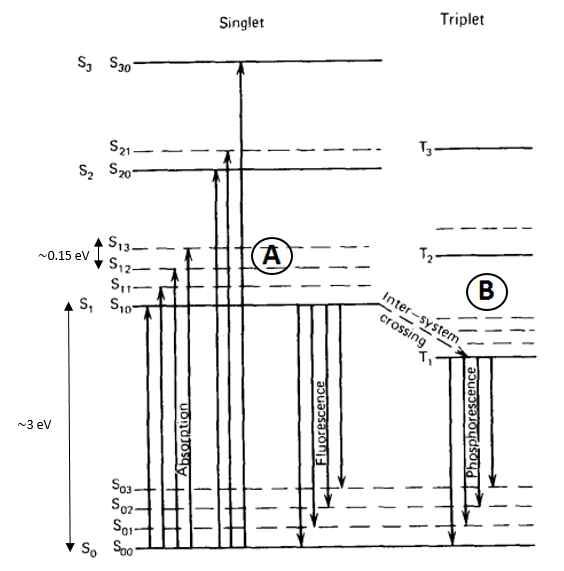
\includegraphics[scale=0.57]{3DesignPrinciples/32Tritium_detector/JablonskyDiagram.png}
\caption{Jablonsky diagram.\label{fig:JablonskyDiagram}~\cite{Knoll}}
\end{figure}

Because of the reason that the distance between all energy levels and sublevels are larger than the termal energy, $0.025~\eV$, non-exciting electrons are in the lowest state $S_{00}$ at STP (standar temperature conditions).

When a particle deposits their kinetic energy on a scintillator, their valence electrons are exited to higher single energetic states very fast (times of the order of picoseconds) which is expressed with upwards direction arrows in the figure \ref{fig:JablonskyDiagram} and they are quickly de-excited to the first single excited state, $S_{10}$, through non-radiactive processes known as internal conversion.

Now, this electrons can de-excited to the fundamental single state, $S_{00}$, through three different physical mechanisms:

\begin{itemize}

\item{} The prompt fluorescence(process A in figure \ref{fig:JablonskyDiagram}), where the electron in the $S_{10}$ energy level  is de-excited to some sublevel of the fundamental state $S_{0i}$, emitting a photon with an energy equal to the energy difference of these levels (around $3$ or $4~\eV$ , visible light). This process happens immediately after the excitation of the scintillator molecules (around tens of nanoseconds after excitation). Each scintillator has a characteristic emission spectrum that defines its response due to the fluorescence mechanism. 

Now we can understand why organic scintillators are practically transparent to their own fluorescense emission. This is because of the reason that there exist a quenching effect in each de-excitation process whereby there are a lost of radiated energy. Due to that, all emmited  photons by the scintillator have less energy than the required energy for excitation. This effect is called Stokes shift and it's represented with a general wavelenght spectrum in the figure \ref{fig:StokesShift}.

\begin{figure}[htbp]
\centering
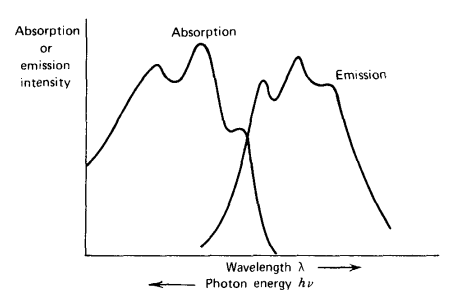
\includegraphics[scale=0.7]{3DesignPrinciples/32Tritium_detector/StokesShift.png}
\caption{Stokes shift.\label{fig:StokesShift}~\cite{Knoll}}
\end{figure}

One of the most important parameters in nuclear physics is the scintillation yield, whcih is the fraction of particle energy that is converted in light. All mechanisms which don't produce prompt fluorescence, like phosphorescence or delay fluorescence, which we will see later, or even internal conversion, contribute to reduce this parameter. The signal of the scintillator depends on the type of particle so, the scintillation yield will be different. This factor is normally given by the manufacturer for mips (minimum ionized particles, that's, for example, electrons with $500~\keV$ or more) in number of photons per $\MeV$.

The intensity of the fluorescence emission in an organic scintillator during time is a combination of two exponential functions, one associated with the lifetime of the level, $\tau$ (on the order of nanoseconds), and the other associated with the energetic level population, $\tau_1$ (on the order of picoseconds).

\begin{equation}
I=I_0\left(e^{t/\tau} - e^{t/\tau_1}\right) \cite{Knoll}
\label{eq:IntensityTimeScintillator}
\end{equation}

\item{} The phosphorescence, where the electron that is in the first single excited state cross to a triple excited state (process B in figure \ref{fig:JablonskyDiagram}) with a process called "intersystem crossing". This is a metastable state with a much longer lifestime so electrons in this state are de-excited to the $S_{0i}$ state, emitting a photon much later than phosphorescence. This process can happen up to $10^{-3}$ seconds after scintillator excitation.

\item{} Delayed fluorescence, which occurs when an electron is in a triple excited state but whose transition to the ground state is forbidden. In this case, this electron can interact with another that is in a similar state and return to the first single state ($S_{1}$ is a more energetic level than $T_{1}$) and quickly de-excited to the ground state. 

\begin{equation}
T_{1} ~+~ T_{1}~ \longrightarrow ~ S_{1} ~+~ S_{0} ~+~ phonons
\label{eq:DelayFluorescence}
\end{equation}

This emission has the same emission spectrum as immediate fluorescence, but occurs later.

\end{itemize}

The scintillating detectors generally use the prompt fluorescence light as output signal so a good scintillator should increase it and reduce other possible physical mechanisms.\label{subsec:PlasticScintillators}
		%\newpage
		
			%\subsubsection{Plastic scintillation fibers}
			Plastic scintillators are organic scintillators that has been disolved in a solven and polimerized. They are easy to machine and can take any desired shape during construction. Among the forms most used today we can find blocks, thin sheets, cylinders, etc.

In our experiment we have been working with an plastic scintillator in the form of fiber, specifically, commercial fibers BCF-12 from Saint-Gobain Crystals Inc \cite{DataSheetBCF12Fiber}. This type of fiber was chosen as the result of a comparative study among some of the best-known commercial manufacturers, such as Kuraray. 

The BCF-12 fibers consist of a scintillated core, whose material is polystyrene, one of the most used solvents for plastic scintillators \cite{Knoll}, with the posibility of surounding it of a cladding of polymethylmethacrylate (PMMA) (smaller refractive index than core in order to archieve a critical angle) or a multicladding (second cladding) with even smaller refractive index.

When a particle deposits all or part of its kinetic energy, some photons are produced in the fiber core as a result of the scintillating process. The quantity of photons which are produced depend on the scintillation yield, whose value is around $8000$ photons per $\MeV$ for a mip in our case (BCF-12 fibers) . It means that, for instance, for tritium electron, this fibers will release a maximum of around 148 photons (when tritium electron has the maximum energy, $18.6~\keV$), probably less because electrons with these energies are not mips.

These photons will shape the useful part of the response of the scintillator (fluorescence) for us. The energy (or wavelength) of these scintillated photons follows the distribution of their emission spectrum which, for the used fibers, is shown in the figure \ref{fig:EmissionSpectrumFibers}.

\begin{figure}[htbp]
\centering
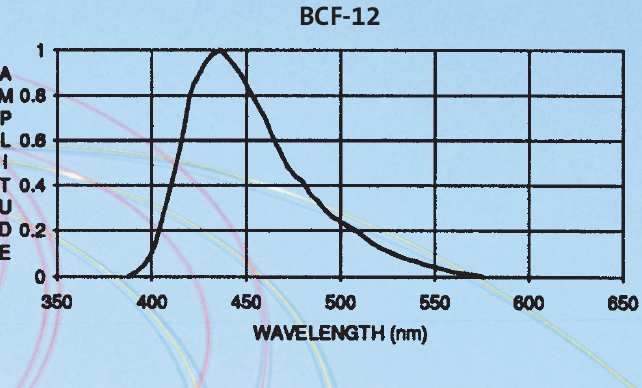
\includegraphics[scale=0.5]{3DesignPrinciples/32Tritium_detector/EmisionBCF12.png}
\caption{Emission spectrum of BCF-12 fibers of Saint-Gobain.\label{fig:EmissionSpectrumFibers}~\cite{DataSheetBCF12Fiber}}
\end{figure}

After the production of scintillated photons, we need to guide these photons to the sensitive part of the photosensor where we will detect them with some probability. Fibers (and scintillators in general) use the optical property of Snell's law \cite{Snell} to guide their photons to the desired part (the ends of the fibers). It is based on the interface created between the core and the surrounding material. When a photon hits this interface, it is refracted (and therefore lost) following the Snell equation, \ref{eq:Snell}. If the surrounding material has a lower index of refraction than the core of the fiber, there exist a critical angle, $\theta_c$, at which, for angles equal or larger than this one, the photons will be totally refracted (and therefore conserved in the fiber for being guided). This effect is showed in the figure \ref{fig:Fiber_physic}.

\begin{equation}
n_0~sen(\theta_0) = n_1~sen(\theta_1) \longrightarrow \theta_c = asen\left(\frac{n_1}{n_0} \right)
\label{eq:Snell}
\end{equation}

There exist a parameter which define the efficiency of the scintillator in order to guide photons, the trapping efficiency. For BCF-12 fibers is between $3.44\%$ and $7\%$ (depending if the event was detected near the fiber axis (minimum) or near the core-clad interface(maximum)).

Therefore, from these $148$ photons initially created with the tritium electron with the maximum energy, only a maximum of around 10 photons (for maximum trapping efficiency) will arrive to our photosensor. As you can see, we work with very weak detector signals, where there is more electronic noise and, as you will see in future chapters, we have made a big effort to reduce this electronic noise as much as possible with several technics.

In the figure \ref{fig:Fiber_physic} we can see how a scintilalting fiber works.

\begin{figure}[htbp]
\centering
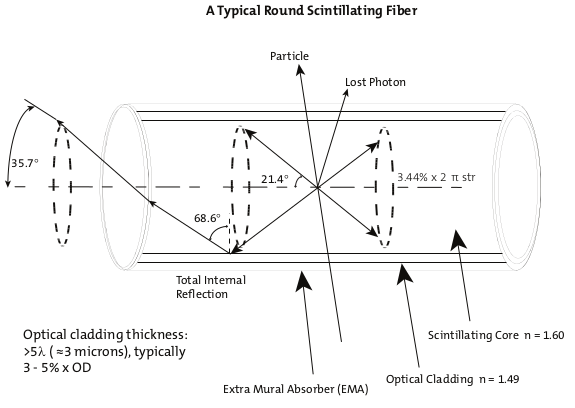
\includegraphics[scale=0.5]{3DesignPrinciples/32Tritium_detector/Fiber_data_sheet.png}
\caption{How photons are collected in a fiber with single clad.\label{fig:Fiber_physic}~\cite{DataSheetBCF12Fiber}}
\end{figure}

The cladding material is useful for protecting the core surface from dirt or aggressive external agents that can reduce the light collection but at the cost of losing some light because it increase the critical angle. In the table \ref{tab:CriticalAngles} we have three different examples where this effect is ilustrated.

\begin{table}[htbp]
%%\centering
\begin{center}
\begin{tabular}{|c|c|c|}
\hline
Material & Refractive index & critical angle ($\degree$) \\
\hline \hline \hline
Air & 1 & $42.98$ \\ \hline
Water & 1.33 & $62.47$ \\ \hline
Cladding of PMMA & 1.49 & $76.26$ \\ \hline
\end{tabular}
\caption{Critical angles asociated to different interfaces created with polystyrene, $n_0=1.6$, and other materials}
\label{tab:CriticalAngles}
\end{center}
\end{table}

This is what theoretically happens but, in the practice, it's difficult to archieve a perfect air-core or water-core interface and it will affect to the light collection. Due to the reason that the commercial claddings are thicker ($30~\micro \meter$) than the mean free path of tritium in water ( around $5~\micro\meter$) we cannot use commercial cladding in our detector hence we will need to take special attencion for archieving a water-core interface enough good. As we will see in the section \ref{}, we have used a special protocol developed in the ICMOL (pie de pagina explicando que es el ICMOL) for preparing fibers before we use them for tritium detection.

Some of the most important properties of the used fibers are summarized in the table \ref{tab:ParametersFibersBCF12}.

\begin{table}[htbp]
%%\centering
\begin{center}
\begin{tabular}{|c|c|c|}
%\hline
%Material & Refractive index \\
\hline \hline 
Core material & Polystyrene \\ \hline
Core refractive index & 1.60 \\ \hline
Density & 1.05 \\ \hline
Cladding material & Acrylic (PMMA) \\ \hline
Cladding refractive index & 1.49 \\ \hline
Cladding thickness ($\mu\meter$) & 30 \\ \hline
Numerical aperture & 0.58 \\ \hline
Trapping efficiency & 3.44\% minimum \\ \hline
%No. of H atoms per cc (core) & $4.82 \cdot{} 10^{22}$ \\ \hline
%No. of C atoms per cc (core) & $4.85 \cdot{} 10^{22}$ \\ \hline
%No. of electrons per cc (core) & $3.4 \cdot{} 10^{23}$ \\ \hline
Radiation lenght (cm) & 42 \\ \hline
Emission peak (nm) & 435 (Blue) \\ \hline
Decay Time, (ns) & 3.2 \\ \hline
1/e Length (m) & 2.7 \\ \hline
Scintillator yield (\#$\gamma$/MeV) & $\sim 8000$ \\ \hline
Operating Temperature & $-20\degree C$ to $50\degree C$ \\ \hline
\end{tabular}
\caption{Properties of BCF-12 fibers from Saint-Gobain Inc. \cite{DataSheetBCF12Fiber}}
\label{tab:ParametersFibersBCF12}
\end{center}
\end{table}

%Bunch -> manojo de fibras

%bundle -> haz de fibras%\label{subsubsec:PlasticScintillatorFibers}
			%\newpage
			
		\subsection{The light detection in photosensors} %\label{sec:Photosensors}
		So far we have created the scintillating photons in the core of the fiber, which have been guided to its ends. Now, what we need is the so-called photosensor, which is an element that is able to detect these scintillating photons. Photosensors have a sensitive part that is optimized to detect photons in a range of energy (normally inside of a visible range) with enough efficiency. After that, the photosensors create an electronic signal that carries information about these photons detected, such as their number or their detection time.

One of the most important things in the scintillation detector is that the emission spectrum of the scintillation (figure \ref{fig:EmissionSpectrumFibers} in our case) overlaps as much as possible with the detection efficiency spectrum of the photosensor used, specifically their higher peaks. In this case, the efficiency of this detector,  which is poroporcional to the multiplication of both factors at the same photon energy, will be optimized (the largest).

There are a lot of different photosensors that can be used for this purpose, whose photon detection relies on totally different physical processes, such as photoelectron multiplier tubs (PMTs), silicon photoelectron multiplier (SiPM) or charge-coupled device (CCD).  Each one of these will have different properties and we have to choose the one which fit better for our objective.

Our main proposal for our scintillation detector will be to use SiPM arrays because they are very fast (of the order of $~\nano\meter$) and have high photodetection efficiency (a maximum of around $50\%$) and high gains (multiplication faction of $10^{6}$) with a low voltage supply. On top of that, one of the most important reason of this choice is that SiPM arrays are able to detect a single photon with high efficiency, which is very important since, as we have seen in the seccion \ref{subsec:PlasticScintillators}, just a few photons will arrive to the sensible part of the photosensor. We will test also the PMTs, which are the conventional choice, because they are still interesting since they have lower dark count rate than an equivalent SiPM and some similar properties like its gain.



%A certain portion (in an optimal case nearly 100\%) of the scintillation photons reach the light detector, which has to be sensitive enough to detect a small number of photons. The detector then produces a signal pulse, which has a height proportional to the number of photons hitting the detector. The signal pulse of the detector is processed by the electronics, and as a result a pulse height spectrum is produced (see Section 3.5).

%This spectrum corresponds to the energy spectrum of the detected particles.
\label{subsec:Photosensors}
		%\newpage
	
			\subsubsection{Photoelectron multiplier Tubs (PMTs)}%\label{subsubsec:PMTs}
			Photoelectron multiplier tube is one of the most used photosensors in nuclear physics during last decades. Its main objective, like all photosensors, is to detect the scintillating photons that reach its sensible part and covert it in an electronic signal large enough to be measured. 

In the figure \ref{fig:SchemePMT} we have a schematic drawing where we can see the PMT components and how it works. First of all, as we can see in the figure \ref{fig:SchemePMT}, we need to create electrons that will travel in the medium (electronic signal). To increase the amount of conserved electrons, we need to work inside a vacuum tube. Therefore, the PMT consists of a vacuum tube that has a glass window through which photons will penetrate inside. 

\begin{figure}[htbp]
\centering
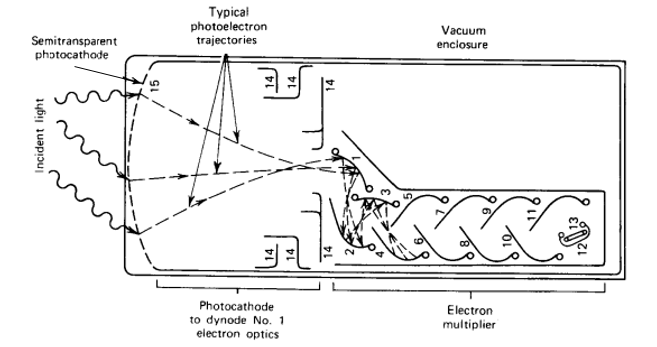
\includegraphics[scale=0.6]{3DesignPrinciples/32Tritium_detector/PMTschematic.png}
\caption{Scheme of a PMT.\label{fig:SchemePMT}~\cite{Knoll}}
\end{figure}

The way in which PMT achieves their aim of detecting scintillating photons happen inside this vacuum tube and it is based in two different phases:

\begin{itemize}
\item{} First, the PMT convert photons that reach its sensible part in electrons, called photoelectrons, with some probability through photoelectric effect. This sensitive part is the photocathode, which consists of a thin layer (thickness of the order of nanometers) deposited on the inner surface of the PMT windows. The material of the photocathode is chosen to increase the probability of producing photoelectric effect with the scintillating photons. The PMTs which we have used in this experiment are the model R8520-406 from Hammatsu \cite{DataSheetPMTs}. The material of the photocathode in our case is Bialkali.

The response of the PMT at long wavelengths is limited mainly because the photon does not have enough energy to produce a photoelectric effect or the emitted photoelectron does not have enough energy to overcome the material-vacuum interface. The response of the PMT at short wavelengths is limited mainly due to absorption in the window material, quartz in our case. Due to both reasons, the response of the PMT will have a strong dependence with the energy of the photon and it's commonly expressed in the quantum efficiency (QE) spectrum which is the quotient between the number of photoelectrons produced at the cathode of the PMT and the number of photons reaching it. For our PMTs, is showed in the figure \ref{fig:QuantumEfficiencyPMT}.

\begin{figure}[htbp]
\centering
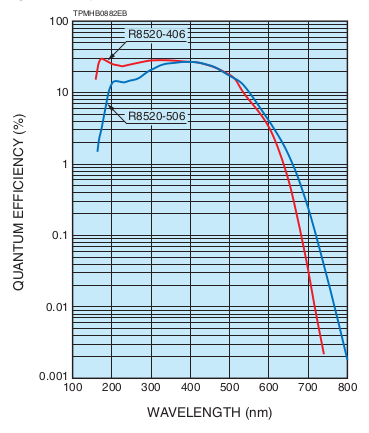
\includegraphics[scale=0.5]{3DesignPrinciples/32Tritium_detector/QuantumEfficiencyPMT.png}
\caption{Quantum efficiency spectrum for the PMT used (R8520-ZB277).\label{fig:QuantumEfficiencyPMT}~\cite{DataSheetPMTs}}
\end{figure}

The maximum values of the PMT quantum efficiency is commonly between $20\%$ and $30\%$ \cite{Knoll} (a little bit less than $30\%$ in our case \cite{DataSheetPMTs}). If we compare the emission spectrum of our scintillating fibers, figure \ref{fig:EmissionSpectrumFibers}, with the quantum efficiency spectrum of the PMTs that we have uses, figure \ref{fig:QuantumEfficiencyPMT}, we can see that the peaks of the spectrum are more or less in the same position ($435~\nm$ for the fibers and $420~\nm$ for the PMT and approximately the same value for $435~\nm$). As I said in the subsection \ref{subsec:Photosensors}, it is very important for increasing the overall efficiency of our scintillation detector. 

\item{} Next, Due to the reason that the number of photoelectrons in the photocatode is very small, we need a electron multiplication stage to achieve a large enough electronic signal to be processed by the electronic system. 

This stage is based on three elements, focusing electrodes, dynodes and anode: They are metallic sheet whose shape and position are designed to optimize the collection of the electrons. The PMT needs a high voltage (HV) which are distributed between all this elements, including the photocathode, in a increasing voltage way in order to attract and accelerate the electrons. This voltage division is achieved with an electronic circuit than can be fed with positive voltage (ground in the photocathode) or negative voltage (ground in the anode). The comercial electronic circuits of Hammatsu are showed in the figure \ref{fig:VoltageDividerCircuit}.

\begin{figure}[htbp]
\centering
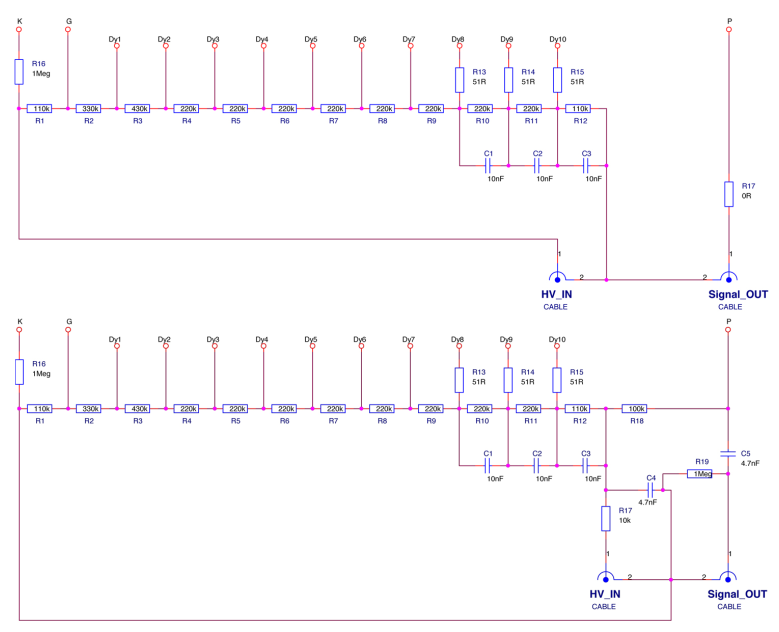
\includegraphics[scale=0.5]{3DesignPrinciples/32Tritium_detector/VoltageDividerPMT.png}
\caption{Hamamatsu commercial voltage divider electronic circuit. Upper circuit with negative supply and lower circuit with positive supply.\label{fig:VoltageDividerCircuit}~\cite{DataSheetPMTs}}
\end{figure}

The electronic circuit that can be supplied with negative voltage is faster due to the ausence of the capacitances C4 and C5, but the other circuit, supplied with positive voltage, can be interesting for other tasks such as measurement of PMT currents. We will use both, depends on the objective of the study.

Focusing electrodes are used to get the photoelectrons to reach the first dinode. Therefore, they have an collection efficiency (CE) that is defined as the quotient between the number of photoelectrons reaching the first dinode and the number of photoelectrons leaving the photocathode and whose value is around $80\%$ for PMTs.

The dynodes is the part where the multiplication takes place. They have different voltage between each dynode in order to accelerate the electrons sufficiently so that, when the electron hit the each dynode, several electrons are emitted. The multiplication factor, $\delta$, is the multiplication of electrons in each dinode and its value is commonly around 5 and it has a strongly dependence with the HV. If we take into accout that the PMT has N dynodes, commonly N=10 and we guess that each dynode has de the same gain, $\delta$, the overall gain of the PMT is:

\begin{equation}
G = CE\cdot{} \delta^N~\cite{Knoll}
\label{eq:PMTGain}
\end{equation}


If we use the numerical values mentioned in this section, we can see that the overall gain of a general PMT will be of the order of $10^6$. It is important to mention that this value depend strongly on the HV used.

We have to take into account that the uncertainty of the output signal with this gain is much greater than without it. That is the reason why, there are some times that it is interesting to work without gain such as when we try to count the number of photons that reach our PMT. We can achieve it with a small modification of the electronic voltage divider circuit \ref{fig:VoltageDividerCircuit}. It consists of short-circuiting all the dindes and the anode. In this way we are collecting the signal in the photocatode in which no amplification has occurred. We will use this voltage divider circuit without gain in our study with fibers.

Finally, when the amplification is used, the anode is the point where the collection of all the electrons produced in this multiplication process takes place and it is the one that gives rise to the output signal of PMTs. 

\end{itemize}

Due to the fact that all intermediate factors (photoelectric effect and multiplication of electrons) are linear, the output signal of a PMT will be linear with the number of photons that reach its sensitive part. It will occur until a large number of photons reach the photocathode at the same time, where saturation will occur and linearity will be lost. This limit depend on the specifically PMT which we are using. This output signal has a spread of the order of tens of nanoseconds.

The multiplication of electrons can be described as a Poisson statistical process, so, for each electron in the first dinode, we will have G new electrons whose variance will be approximately $\sqrt{G}$.

Finally, we have to take into account that the photocathode can emit electrons whose origin doesn't belong to the scintillation light. This signal, which is named dark current, can  happen due to several reasons like cosmic radiation, light from environment or thermoionic emission (the dominant) and, for our PMTs, this value will be around $2~\nano\ampere$ according to Hammamatsu data sheet.

The calibration of the most important parameters (for our objective) of the PMTs used, which are dark current, gain for several HV and quantum efficiency,  have been done at IFIC in the framework of NEXT experiment \cite{CalibrationPMTsNEXT}. \label{subsubsec:PMTs}
			%\newpageand
		
			\subsubsection{Silicon Photoelectron Multiplier Array (SiPMs array)}%\label{subsubsec:SiPMs}
			The Silicon Photomultiplier (SiPM) is a photosensor, based on semiconductor materials, which has been developed in recent decades and they are replacing conventional PMTs in some experiments or applications. They have been designed to archive outstading photon-counting capabilities better than conventional PMTs with high gain and high photodetection efficiency equal to or larger than conventional PMTs but with some important differences like insensitiveness to magnetic fields, low operating voltage, compactness among other differences.

\textbf{Semiconductor materials} 

Silicon is a semiconductor material and, like any semiconductor material, it has an electronic band structure that consists of two bands: Valence band and conduction band which are separated by a forbidden energy gap (with width of around $1~\eV$ for semiconductors \cite{Leo}) where there cannot be electrons. These energy bands are based on many energy levels that are so close that we can consider a continuum. You can see a diagram of these bands in Figure \ref{fig:EnergyBandsSC}.

\begin{figure}[htbp]
\centering
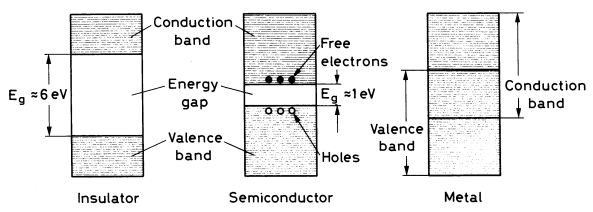
\includegraphics[scale=0.6]{3DesignPrinciples/32Tritium_detector/Energy_bands_isolate_semiconductor_conductor.png}
\caption{Energy band scheme for (a) insulator, (b) semiconductor and (c) conductor.\label{fig:EnergyBandsSC}~\cite{Leo}}
\end{figure}

Electrons in the conduction band, unlike those in the Valence band, can move freely in the material so they contribute to the electric current. 

Silicon has four electrons in their valence band (tetravalent atom) so it form four covalent bounds creating a cristal lattice ($\ce{Si_2}$). Normally a small quantity of impurities ($10^{13}$ atoms/$cm^3$) are added to modifying this lattice, that's dopping the material. 

If the dopant has 5 valence electrons (pentavalent atom like phosphorus or arsenic) there will be a free electron which will be at an energy level created in the forbbiden band, very close to the conduction band. It is called "n-type" semiconductor and the electrons are the majority charge carriers.

Otherwise, if the dopant has 3 valence atoms (trivalent atom like gallium or boron) it will have a hole\footnote{Electron absence in the crystal lattice} that will be at an energy level created in the forbidden band, very close to the valence band. In this case, the holes are the major charge carriers and this element is called "p-type" semiconductor.

Both configurations (p-type or n-type semiconductor) are shown in the figure \ref{fig:NPType_SC}.

\begin{figure}[htbp]
\centering
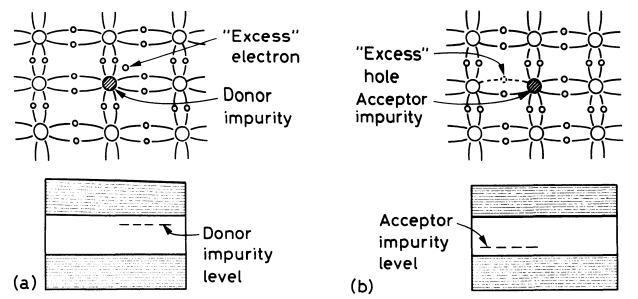
\includegraphics[scale=0.6]{3DesignPrinciples/32Tritium_detector/N_P_type_semiconductors.png}
\caption{Crystal lattice and energy band scheme formed by a silicon with (left) a pentavalent dopant that creates an n-type semiconductor (right) a trivalent dopant that creates a p-type semiconductor. \label{fig:NPType_SC}~\cite{Leo}}
\end{figure}

SiPM is based on a silicon diode formed by a junction of n-type and p-type semiconductors that is made with special techniques to archive a good contact between both surfaces.

This union creates the so-called depletion zone, which is the interface between both materials. In this zone, there are a diffusion of electrons to the p-type semiconductor and holes to the n-type semiconductor due to the difference in the concentration of the majority charge. This re-arrange of the charge creates an electric field in the depletion zone contrary to the movement of these charges, whose potential difference, called contact potential, is $V_0 = 0.7~\volt$ for silicon \cite{Leo}. All this information is shown schematically in the figure \ref{fig:DiodeScheme}

\begin{figure}[htbp]
\centering
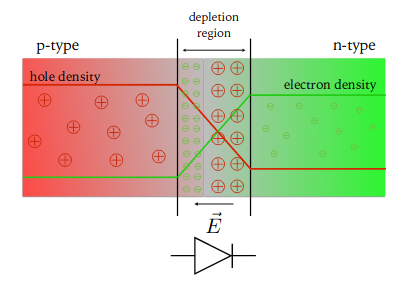
\includegraphics[scale=0.6]{3DesignPrinciples/32Tritium_detector/SchemeSiPMDiodo.png}
\caption{(Above) Schematic of the charge distribution and electric field created in a pn-junction. (Bottom) Commonly used symbol for a diode.\label{fig:DiodeScheme}~\cite{TesisNEXTSiPMs}}
\end{figure}

There are no charge carriers in the depletion zone and, if any one are created, they will be swept out by the electronic field (special interesting property for radiation detectors since charge carriers are created in this zone when ionizing radiation crosses through it).

If we want to use this p-n junction as a particle detector, this setup has some problems that we have to overcome. On the one hand we need to prevent the charge recombination in order to optimize its collection in the depletion zone. On the other hand we need to increase the width of the depletion zone (it is $0.5~\micro\meter$, too small to stop interesting particles) and, as we will see in the section \ref{sec:CharacterizationSiPM}, this small width increases the capacitance value that will increase the noise in the output signal.

We managed to overcome these problems if we apply a bias voltage across the junction. If this bias voltage is with positive terminal in p-type semiconductor and negative terminal in n-type semiconductor, which is called forward bias voltage, it will create an additional electric field opposite the internal electric field, which will attract electrons in n-type towards p-type and holes in p-type towards n-type. In short, it will reduce the depletion zone, and if the applied voltage is greater than the contact potential, an electric current will be created even if no charge has deposited their energy in the depletion zone.

However, if this bias voltage is applied with positive terminal in n-type semiconductor, negative terminal in p-type semiconductor, which is called reverse bias voltage, the contrary effect will happen and the intensity of the electric field in the depletion zone will be increased. This effect will be limited by the resistence of the semiconductor and if we use a too large bias voltage the pn-juntion will breakdown and it will begin conducting. 

If reverse bias voltage is applied, we can solve all the problems mentioned above. In this case, the charge collection will be improved and the width of the depletion zone will be increased. If ionizing radiation crosses the depletion zone, which is wide enough to detect interesting particles, it will deposit their energy and, due to that, charge charriers will be created\footnote{The energy required to create an electron-hole pair in silicon is $3.62~\eV$ in STP\cite{Leo}} which will be swept due to the electric field and an optimized current signal will be created. 

Depending on the intensity of the polarization voltage we can work in different modes and we will have different output signals. If the bias voltage is less than the threshold, the charge carriers will recombine and no output signal will be produced. If the bias voltage is larger than threshold an avalanche is created due to each original electron and it is independent of other possible avalenches. Due to this avalanche, it has a gain whose valuer is around $200$. This mode is called proportional mode since the collected charged is proportional to the energy deposited. Finally, If the bias voltage is even larger, each avalanche can trigger a second avalanche and, due to that, their internal gain is higher than the proportional mode\footnote{The gain of commercial SiPMs, for example Hammamatsu, is of the order of $10^6$, similar to the PMTs}, that's, it's output signal will be larger. This mode is called Geiger mode since the output signal only show when a detection has happened but it is not proporcional to the energy deposited. 

The voltage at which the SiPM changes from proportional to geiger mode is called the breakdown voltage, $ V_ {BR} $. If it works at a lower voltage it is in proportional mode but if it works at a higher voltage, it works in geiger mode. The measurement of the breakdown voltage is one of the most important things to characterize the SiPM and I show how we have done it in the section \ref{sec:CharacterizationSiPM}.

\textbf{Silicon photomultiplier}

The SiPM is based on a matrix of APDs which are photodiodes operating in geiger mode. A scheme of an APD used in a SiPM is shown in the figure \ref{fig:SchemeAPD}. It has p+ and a n+ layers\footnote{p+ and n+ layers are the same as p and n layers, explained before, but with higher concentrations of acceptor impurities or donor impurities respectively CHECK THAT!!} that are used because they improve the properties of SiPMs but the way these APDs work is the same as that described before. 

\begin{figure}[htbp]
\centering
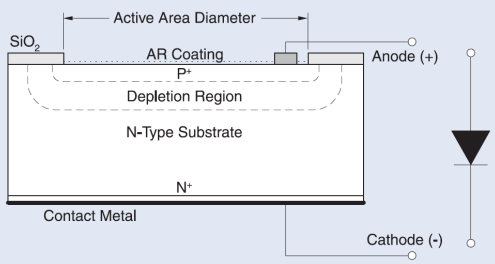
\includegraphics[scale=0.6]{3DesignPrinciples/32Tritium_detector/APD_scheme.png}
\caption{Scheme of a APD and electrical symbol used.\label{fig:SchemeAPD}~\cite{OSI}}
\end{figure}
 
These APDs, called pixels when they are part of a SiPM, are connected in parallel and we read the sum of all of them at each moment. The output signal of each pixel is approximately the same regardless of the energy deposited, with some difference due to the uncertainty in the SiPM manufacturing process and the statistical nature of the detection process. Due to that, we cannot know the energy deposited in each APD but, as we read all SiPM pixels at the same time, as you can see in the figure \ref{}, the charge on the output signal when we detect n photons simultaneously will be n times the charge we have when we detect only one photon. Due to this property, after a correct calibration of our SiPMs which will be shown in the section \ref{sec:CharacterizationSiPM}, we can know how many particles (photons in our case) we have detected, which have a linear relationship with the output signal. 

Furthermore, as we saw in section \ref{subsec:PlasticScintillators}, since we work with scintillators, in our case, the number of photons is proportional to the deposited energy, so we can recover the characteristic linearity of its output signal and to know the energy deposited in our scintillator, and, therefore, the energy of the initial radioactive event, which will be one of the most important parameters in our signal.

\begin{figure}[htbp]
\centering
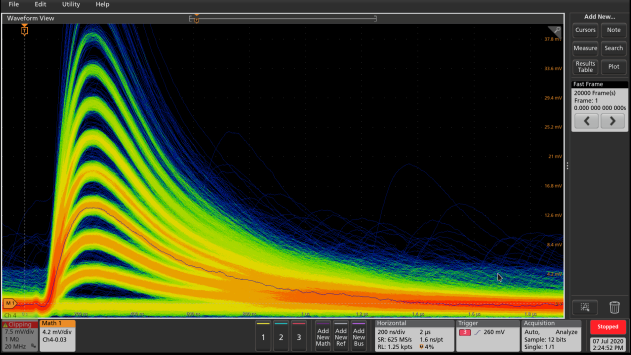
\includegraphics[scale=0.6]{3DesignPrinciples/32Tritium_detector/Several_SiPM_pulses.png}
\caption{Using persistence on the oscilloscope to show several pulses with different heights. Each height associated with a different number of  SiPM pixels lit at the same time.\label{fig:PulsesOfSiPM}}
\end{figure}

On top of that, these pixels need to be so small\footnote{Pixel sizes for commercial SiPMs are $50$ or $75\mu\meter$ \cite{DataSheetHammamatsu_1_SiPM_50}, \cite{DataSheetHammamatsu_1_SiPM_75}} that, if the photon density to be detected is low enough, we only detect one photon in each pixel. If it doesn't happen, we will detect two or more photons with the same pixel but the output signal will be the same as one detected photon, so we will have a loss of linearity of our output signal. This effect is known as saturation and it is important to know the photon density at which it happens for our SiPMs. The experimental measurements of this effect, which have been done for our SiPMs, is shown in the section \ref{sec:CharacterizationSiPM}. SI LA MIDO YO PERFECTO, SI NO PONER UNA FOTO DE LA TESIS LARGA.

Each of these pixels has a quenching resistance\footnote{The tipical valuer of this quenching resistance for commercial SiPMs is around $500~\kilo\Omega$} in series that is used to stop the current produced when this pixel has detected a particle. It is used for limit the current drawn by the diode during breakdown and reduce the reverse voltage seen by the diode to one below the breakdown voltage. After that, the voltage seen by the diode is reset to the bias voltage and this pixel is ready to detect a new particle again. In figure \ref{fig:ChenchingResistance} (left) a diagram of these chenching resistances and APDs in a SiPM and (right) how it works is shown respectively.

\begin{figure}[htbp]
\centering
{
%\subfloat[PDE]
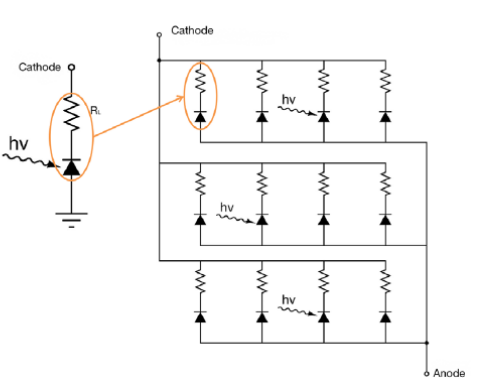
\includegraphics[scale=0.35]{3DesignPrinciples/32Tritium_detector/Quenching_resistence_of_a_SiPM_scheme.png}
%\caption{Simple electronic model of a SiPM.\label{fig:ElectricModelSiPM}~\cite{DataSheetSensL}}
}
{
%\subfloat[Espectro de emisión]
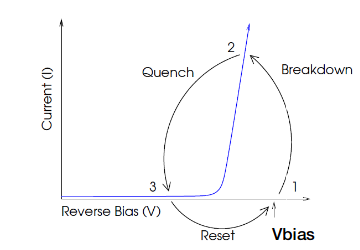
\includegraphics[scale=0.5]{3DesignPrinciples/32Tritium_detector/How_a_quenching_resistence_in_a_SiPM_works.png}
%\caption{Output current of a SiPM as a function of the reverse voltage. It show that the quenching mechanism is essential for working with SiPMs\label{fig:HowSiPMworks}~\cite{DataSheetSensL}}
}
\caption{(Left) Electronic scheme of a SiPM and (right) output current of a SiPM as a function of the reverse voltage. It show that the quenching mechanism is essential for working with SiPMs\label{fig:ChenchingResistance}~\cite{DataSheetSensL}}
\end{figure}

In this simple electrical scheme we can see that all pixels have a common cathode and anode which means that, as we said before, they are at the same bias voltage and the output is the sum of all of them.

We have a lot of names to refer to these photosensors such as SiPMs, MPPCs, G-APDs, SSPMs, MRS-ADPs or AMPDs. The candidate for TRITIUM project is S13360-6075 from Hamamatsu photonics \cite{DataSheetHammamatsu_1_SiPM_75} because its characteristics are the ones that best fit our objectives since this model has super low afterpulses, crosstalk and dark counts than other SiPM models from Hammamatsu. Its characteristics and properties are shown in the table \ref{tab:PropertiesOfSiPM75}. 

\begin{table}[htbp]
%%\centering.
\begin{center}
\begin{tabular}{|c|c|}
\hline
Parameter & Numerical value \\
\hline \hline \hline
Serie & $S13360$ \\ \hline
Model & $6075$ \\ \hline
Pixel Pitch ($\mu\meter$) & $75$ \\ \hline
Effective photosensitive area ($\mm^2$) & $6.0 \times 6.0$ \\ \hline
Number of pixels & $6400$ \\ \hline
Fill factor & $82\%$ \\ \hline
Refractive index of windows material & $1.55$ \\ \hline
Operating temperature range ($\degree C$)& $[-20,60]$ \\ \hline
Spectral response range, $\lambda$ ($\nano\meter$) & $[320, 900]$ \\ \hline
Peak sensitivity wavelength, $\lambda_p$ ($\nano\meter$) & $450$ \\ \hline
PhotoDetection Efficiency, PDE, $\lambda=\lambda_p$ ($\%$) & $50$ \\ \hline
Dark counts, Typical/Maximum (kcps) & $2000/6000$ \\ \hline
Terminal capacitance, $C_t$ ($\pico\farad$) & $1280$ \\ \hline
Gain, M, & $4 \cdot{} 10^6$ \\ \hline
Breakdown Voltage, $V_{BR}$ ($\volt$) & $53$ \\ \hline
Cross talk probability($\%$) & $7$ \\ \hline
Temperature coefficient $\Delta TV_{op}$ (m$\volt/\degree C$) & $54$ \\ \hline
\end{tabular}
\caption{Characteristics of SiPM S13360-6075 from Hammamatsu Photonics \cite{DataSheetHammamatsu_1_SiPM_75}.}
\label{tab:PropertiesOfSiPM75}
\end{center}
\end{table}

These characteristics and properties will be explained and their experimental measurements will be shown in section \ref{sec:CharacterizationSiPM}. These numerical values, which appear in the table \ref{tab:PropertiesOfSiPM75}, are provided by Hammamatsu photonics but it is only an approximation for this model. These parameters must be determined experimentally for each SiPM used because it can be very different even if it is the same model.

It must be taken into account that we will do this characterization at the level of a single SiPM because, at the beginning, it is easier to understand the results but we will work with a matrix of them and we will have to do this characterization for each matrix used. 

The matrices under consideration are the model "S13361-6050" from Hammamatsu, which consists of a $4\times 4$ SiPM matrix where the active area of each SiPM is $6\times 6~\mm$ \cite{DataSheetHammamatsu_array_SiPM_6050} or the model "S13361-3050" from Hammamatsu, which consists of a $8\times 8$ SiPM where the active area of each is $3\times 3~\mm$ \cite{DataSheetHammamatsu_array_SiPM_3050}. They are a commercial matrices from Hammamatsu and, as you can see, the total active area that we will cover with these arrangements is the same in both cases, $24\times 24~\mm$ and it is approximatelly the same that the active area covered with the PMTs used, which has been shown in the previous section.

These matrices have a common bias voltage and common ground for all SiPMs that are contained and we will have an output signal for each SiPM. 

We hope to obtain better results with the 4x4 matrix for theoretical reasons which we will see in the section \ref{sec:CharacterizationSiPM} like larger PDE, mainly due to a larger active area but it is something that we will have to verify with experimental measurements.




Nuestro SiPM esta dopado? con que?\label{subsubsec:SiPM}
			%\newpage
			
			\subsubsection[Comparison photosensors]{Comparison of photosensors considered}%\label{subsec:SiPMs}
			As we have said before, we are going to use two of the most widely used photosensors in the world, PMT and SiPM. Each has some properties that are better than the other for our experiment and its own problems. We will have to test both and choose the one with which we achieve better results.

The output signal of both photosensors used is proportional to the number of incident photons and they have a similar internal gain (of the order of $10^6$). Both properties are essential for our experiment in order to detect tritium events and obtain a signal large enough to be measured and processed. 

They have fast output signals, whose rise time is shorter than nanoseconds, and a wide spectral sensitivity that is similar for both ($[200-800]~\nano\second$ for PMT and $[300-900]~\nano\second$ for SiPM).

The supply voltage necessary to work with SiPM, on the order of tens of volts, is much lower than that of PMTs, which require high voltage, that is, on the order of thousands of volts and the PDE at $420~\nano\meter$,  achieved with SiPM is higher, around $50\%$, than PMT, whose PDE is around $30\%$. A large PDE is essential because, as we have seen before, the number of photons that we will read in each tritium event will be very low, so we must detect as many photons in each event as we can.

Furthermore PMTs, due to the reason that they consist of a vacuum tube, are more bulky and fragile than SiPMs, which are compactness and robust. It is an advantage of the SiPMs because we want that our detector work during a lot of years so we need this to be durable. Furthermore, because PMTs are manually produced, they are much more expensive, thousands of euros, than SiPMs, tens of euros, which can be mass produced.

On top of that the behavior of the PMTs is affected by magnetic fields, something which doesn't happen with SiPMs with which it has been tested that it can work correctly with magnetic field intensities between 0 and 7 Tesla. 

In addition to that, due to their enormous uniformity, SiPMs are capable of distinguishing the exact number of photoelectrons detected and even resolving a spectrum of a single photoelectron, which is not possible with PMTs due to variations in their gain.

On the other hand, the dark current rate for PMTs is much lower (a few counts per second) than for SiPMs, whose dark current rate is between 0.1 and 1 Mcps\footnote{Mega counts per second, $10^6$c/$\second$} (depends on its size) and it happens almost entirely at the level of a single photoelectron. It is a problem of the SiPMs because we need to distinguis the tritium signal from this background. In addition to that, SiPMs have other properties, such as the crosstalk of the afterpulses, that must be measured and extracted since they can affect the correct measurement. We will see how to do it in the section \ref{sec:CharacterizationSiPM}

Also, the SiPMs output signal is affected by a slight change in temperature, something which doesn't happen with PMTs. It is a serious problem of the SiPMs for our experiment because we will work in the field, where we cannot avoid such a low temperature change. As we will see in section \ref{sec:CharacterizationSiPM} we will solve this problem with a suitable change in the supply voltage that compensates for this variation.\label{subsubsec:ComparisonPhotosensors}
			\newpage
					
		\subsection{Readout system of photosensors}\label{subsec:Electronic}
			%\subsubsection{Introduction}
			Ver tesis de detectores monolíticos.\label{subsec:IntroductionHemos hablado ElectronicalSystem}
			%\newpage
	
			\subsubsection[Electronical system for PMTs]{Electronical system for PMTs}
			In the different tests in which we have used PMT, we were interested in two different main objectives. On the one hand, we were interested in knowing the amount of incident photons that reached the PMT photocathode, which can be interesting, for example, to characterize fibers, and, on the other hand, we were interested in the energy of each event that occurred, which can be interesting, for instance, to obtain an energy spectrum or to discriminate events based on their energy (for knowing the origin of these events and counting only interesting events).

In the first case, if we want to know how many photons have reached the photocathode, we have to work without the internal gain of the PMT. The reason for this is that it introduces a large uncertainty in the measurement. The use of this internal gain could be interesting in other situations such as when we need to know the energy of the event because, as we saw in the section \ref{subsubsec:PMTs}, its use greatly enlarges our signal, a factor of the order of $10^6$, and, due to that, it is easier to process and analyze it.

For working without the internal gain of the PMT we need to avoid the use of the electron multiplication stage that we saw in section \ref{subsubsec:PMTs}. To achieve this, we design, build and test special PCBs, whose electronic scheme is shown in figure \ref{}, in which we short-circuit all the dindes and read the signal directly from the photocathode.

PHOTO AND ELECTRONIC DESIGN.

This PCB is designed to be powered with positive supply voltage which is less thant the normal situation $[0-400~\volt]$. The reason of this lower supply voltage is that we don't need to create a voltage difference between each pair of dynodes in the chain (we only need to create a voltage difference between the photocathode and the first dinode).

In this case, the output signal of our photosensor is very fast and small (currents of the order of tens of nanoamperes\footnote{$1~\ampere=10^{9}~\nano\ampere$}) and we need a special system to analyze these types of currents. The system which we have chosen is Keithley 6487 Picoammeter/Voltage Source \cite{DataSheetKeithley6487}, which is a commercial system from the Keithley company, because it has some interesting options for this study such as automatic baseline correction, the ability to read signals as small as picoamps and the ability to perform some interesting mathematical operation, such as the average of N measurements with the associated statistical error, where N is programmable by the user ($N=100$ in all our studies).

With this configuration we can measure the output current of our photosensors and, from it, quantify how many photons have been detected by the PMT photocathode using the equation \ref{eq:NumPhotonsFromIntensityPMT}:

\begin{equation}
Nº\gamma/\sec = \frac{\left( I_{PMT} - I_{DC} \right)}{q_e \cdot{} QE \cdot{} CE}
\label{eq:NumPhotonsFromIntensityPMT}
\end{equation}

Where $I_{PMT}$ is the output current of the PMT when it detects photons and $I_{DC}$ is the dark current of the PMT. This equation takes into account the quantum efficiency, which is close to $30\%$ for the PMTs used, and the capture efficiency in the dyndes, which is equal to 1 because we read the signal directly from the photocathode. In addition, it is taken into account that, due to the photoelectric effect in which this detection consists, each detected photon only generates one electron, whose charge is $q_e$.

In the second case, if we want to know the energy of the event that occurred, we need to work with the internal gain of the PMT. For that we will use the electron multiplication stage that we saw in section \ref{subsubsec:PMTs}.

In all our studies we have used several PMTs in our experiments (two or four depend on the case). The electronic schematics used, which are shown in figure \ref{} and \ref{} respectively, are based on various NIM technology modules\footnote{The Nuclear Instrumentation Module (NIM) is a standard specification convention for electrical and mechanical parameters defined in electronic modules used in experimental nuclear and particle physics.}.

\begin{figure}[htbp]
 \centering
  \subfloat[Event detected in only one PMT.]{
   \label{subfig:signalInOnePMT}
    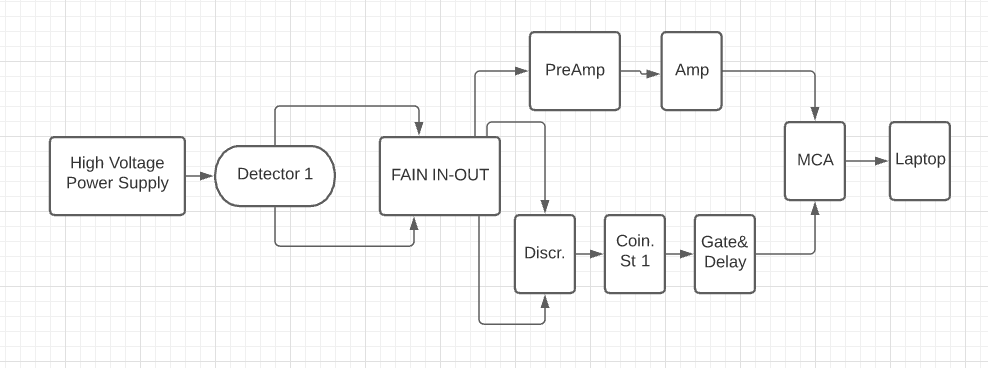
\includegraphics[width=1.0\textwidth]{3DesignPrinciples/32Tritium_detector/Electronical_Scheme_1_detector.png}}
    \newline
  \subfloat[Event detected in two PMTs, one detector.]{
   \label{subfig:signalInTwoPMTOneDetector}
    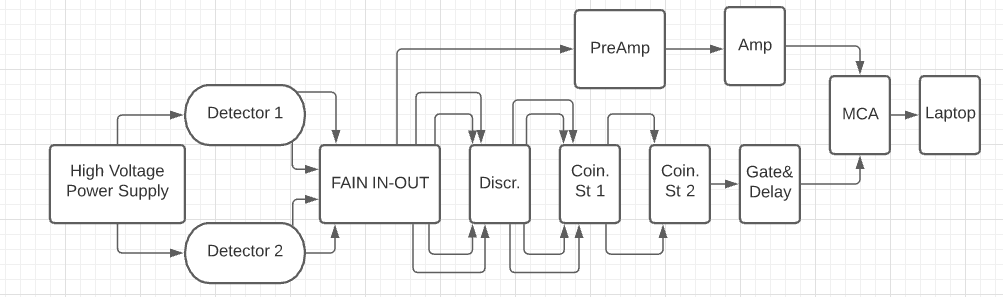
\includegraphics[width=1.0\textwidth]{3DesignPrinciples/32Tritium_detector/Electronical_Scheme_2_detectors.png}}
 \caption{Different situation that can happen when we do time coincidences with PMTs.}
 \label{fig:DifferentCoincidences}
\end{figure}

The PMTs used in each situation are feeded with the voltage supply "TC 952 High Voltage Supply" from Tennelec \cite{DataSheetHVSupplyTennelec}. It has four channels for feeding up to four different PMTs so it is enough for both configurations. In some situations we need to work with both configurations at the same time, that's, with six PMTs at the same time.  In this cases other voltage supply had been used, called  "HV Power Supply N 1130-4" from "Wenzel Elektronik" \cite{DataSheetHVSupplyWenzel} company with which we get 4 additional channels for feeding PMTs. The high voltage used in each case will be named in each specific situation.

As you can see in the figures \ref{} and \ref{}, in both electronic configurations there are two different paths that must be followed by the output signals of each PMT, the amplification part and the time coincidence part. Therefore, the first module we need is the analogic FAN IN-OUT module which is used to duplicate the input signal.

The module used is the "Quad linear FAN IN-OUT MODEL 740" module from the company "Philips Scintific" \cite{DataSheetFANINOUT}. With this module we can obtain up to 4 output signals (we only need two) that are totally identical to each input signal. For each PMT we have two identical output signals. One will be used as the input for the amplification part and the other will be used as the input for the time coincidence part.

\begin{itemize}

\item{} The amplification part, which is the same for both electronic configurations, figures \ref{} and \ref{}, is used to process and amplify the output signal and it is the same for both configurations. We have to take into accout that we have only used the signal from one PMT for the amplification part. We could have added a stage where we add the four PMT output signals and it would probably improve our results, but since our ultimate goal is to work with SiPM, we have not delved into that.

The electronic path we have followed to achieve this amplification is:

\begin{enumerate}

\item{} In this part we introduce one of the output signals of the previous module (FAN IN-OUT) in a preamplifier that is used to prepare the signal to be amplified, appendix \ref{App:ElectronicModulesNIM}. The preamplifier used is "MODEL 9326 FAST PREAMP" from ORTEC \cite{DataSheetPreAmp}.

\item{} The output signal from the preamplifier is introduced into the amplifier where it will be converted to a positive signal with a shape close to the Gaussian function and an amplification factor will be applied. The amplifier modules used on this studies are "model 575A" and "model 671", both from ORTEC company \cite{DataSheet575Amp}, \cite{DataSheet671Amp}. The output signal for 575A module is shown in figure \ref{fig:InputSignalsMCA}, green color.

\end{enumerate}

\item{} The time coincidence part is used to obtain the coincidence gate that will be used to indicate when we have to save the amplified signal (which is when all the PMT output signals are in time coincidence). Only the saved output signal will be used for the analysis. 

This part is practically the same in both cases with just one additional step when we use four PMTs. The electronic path followed in the time coincidence part is:

\begin{enumerate}

\item{} The second output signals of the FAN IN-OUT module for each PMT are introduced into a discriminator module where we obtain an output logic signal with height of $-1.2~\volt$ and width of $240~\nano\second$ when a threshold, the one programmed by the user, is exceeded. The discriminators used in our experiments are  "Octuple Constant-Fraction Discriminator CF8000" module from ORTEC company \cite{DataSheetDiscriminator} and "4 channels discriminator model 84" from CAEN company. These four output signals are shown in figure \ref{subfig:signalInAllPMTsBothDetector} for four PMTs in coincidence.

\item{} Now is the time to make time coincidences. As we will see in the section \ref{subsec:SetUpActiveShield} and chapter \ref{chap:Prototypes}, we have two photosensors in each detector, so we will do time coincidences in pairs of photosensors, PMTs in this case.

Therefore, each pair of output logic signals of the discriminator module (attached to two PMTs that are in the same detector) will reach a different channel of the coincidence module and generate an output signal, with a height of $-1.4~\volt$ and width of $20~\ns$, when a time coincidence has occurred on them.

This first time coincidence stage is used to remove the detection of  external light or dark current of PMTs from  in the saved measurements. This is because this module only generate logic output signals when both PMTs have detected photons at the same time, indicating that these photons are coming from the coupled scintillator.

The time coincidence modules used are "Coincidence Unit Model 465" from LeCroy \cite{DataSheetCoincidenceLeCroy} and "Coincidence Type N6234" from CERN-NP \cite{DataSheetCoincidenceCERN}.

\item{} The next step, which is included only when working with four different PMTs, is used to do time coincidence between two different detectors. It could be interesting, for exapmle, to detect hard cosmic radiation as we will be in the \ref{subsec:SetUpActiveShield} section.

If we want to do time coincidences between both detectors, we have to use the logical output signals of the previous step (output of the coincidence module) as input of another coincidence stage similar to the previous one. In this case, which is only used when we have four PMTs, we will have a logical output signal with the same parameters, height of $-1.4~\volt$ and width of $20~\nano\second$ when both detectors have detected events at the same time. The modules used is the same named in the previous point.

In the figure \ref{fig:DifferentCoincidences} we have shown all the different situations that we can have with the previous two steps. There we have four logical signals from four PMTs. The two first signals (channel one and two) come from two PMTs connected to one detector and the other two signals (channels three and four) come from PMTs connected to another detector.

\begin{enumerate}
\item{} In figure \ref{subfig:signalInOnePMT} we can see that only one PMT (channel two) has detected an event. As the second PMT connected to the same detector (channel one) did not detect this event, it indicates that the detected photons did not come from the scintillator. In this case, the time windows (output from coincidence module, stage 1) will not be opened and this event will not be saved.

\item{} In figures \ref{subfig:signalInTwoPMTOneDetector} and \ref{subfig:signalInTwoPMTOtherDetector} we can see that two PMT signals connected to the same detector have detected an event but the others have not. It means that it is an event that has only been detected by one detector. If we are using the second stage of time coincidence, the time window will not open to save this event.

\item{} In figure \ref{subfig:signalInAllPMTsBothDetector} we can see that, in this case, all signals have detected the event. It means that it is an event that has been detected for both detectors. In this case, a time window will be created to save this event.

\begin{figure}[htbp]
 \centering
  \subfloat[Event detected in only one PMT.]{
   \label{subfig:signalInOnePMT}
    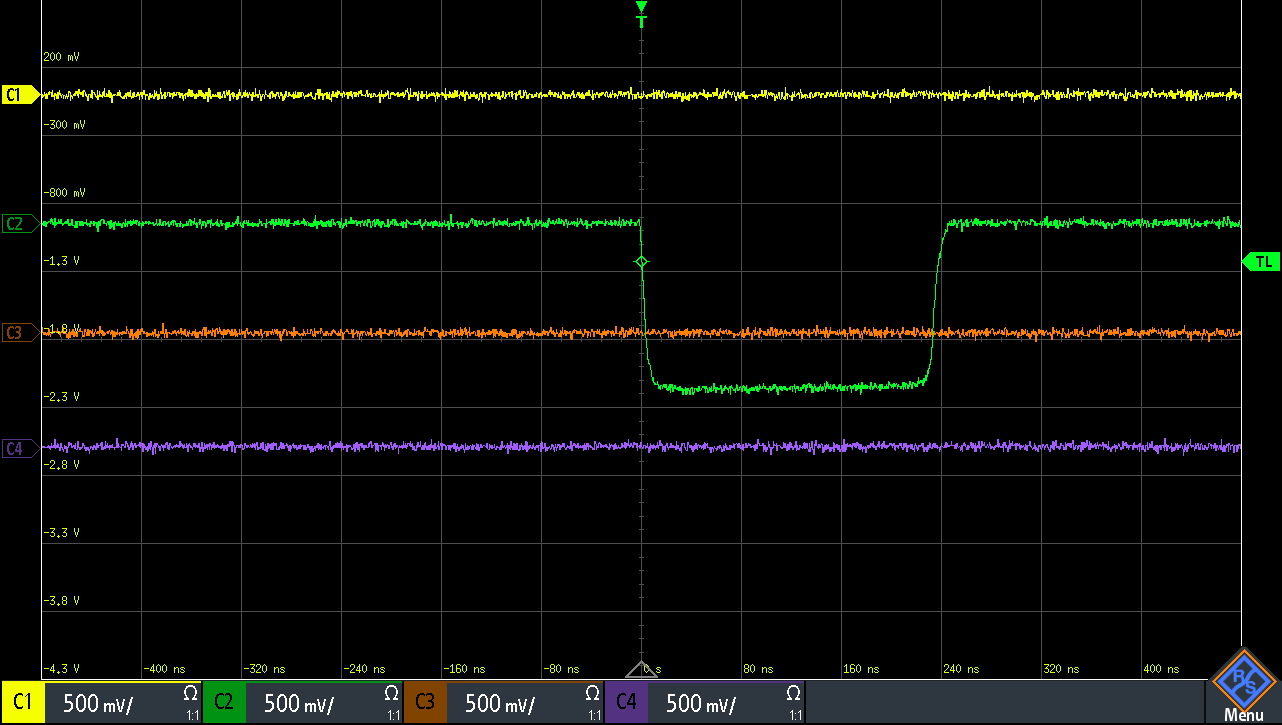
\includegraphics[width=0.5\textwidth]{3DesignPrinciples/32Tritium_detector/1_coincidences.png}}
  \subfloat[Event detected in two PMTs, one detector.]{
   \label{subfig:signalInTwoPMTOneDetector}
    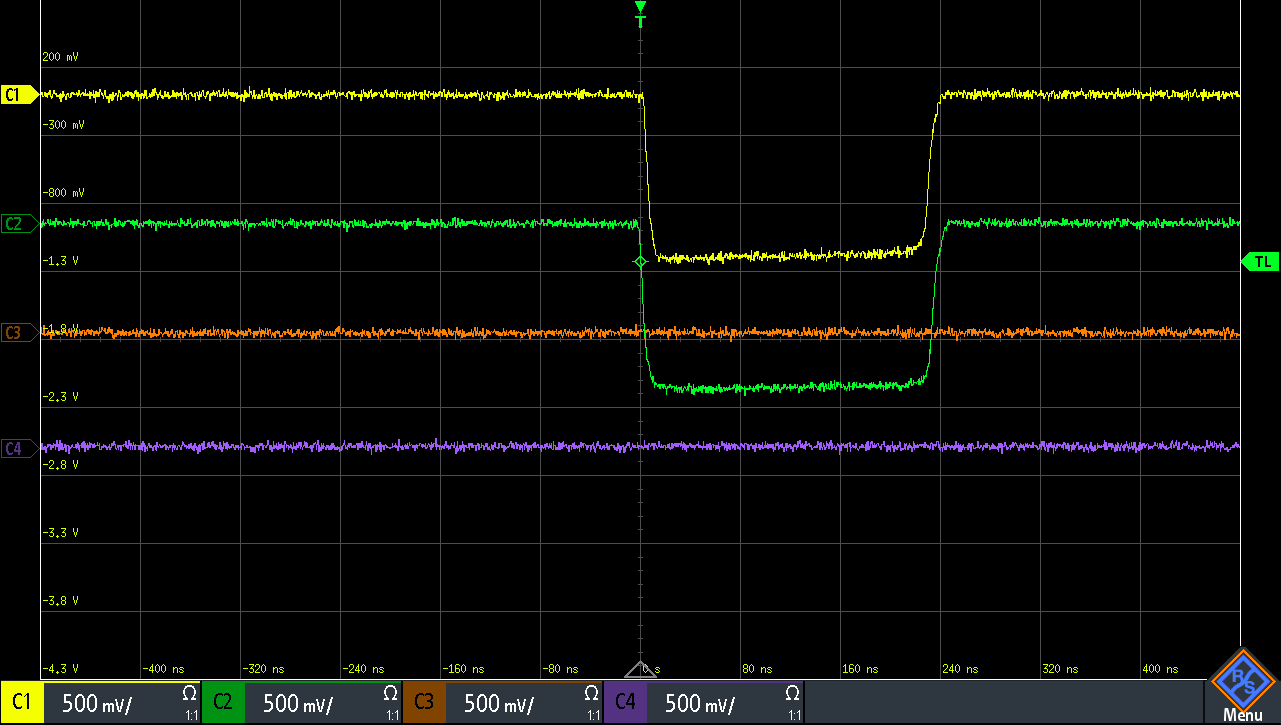
\includegraphics[width=0.5\textwidth]{3DesignPrinciples/32Tritium_detector/2_coincidences_1.png}}
   \newline
  \subfloat[Event detected in two PMTs, other detector.]{
   \label{subfig:signalInTwoPMTOtherDetector}
    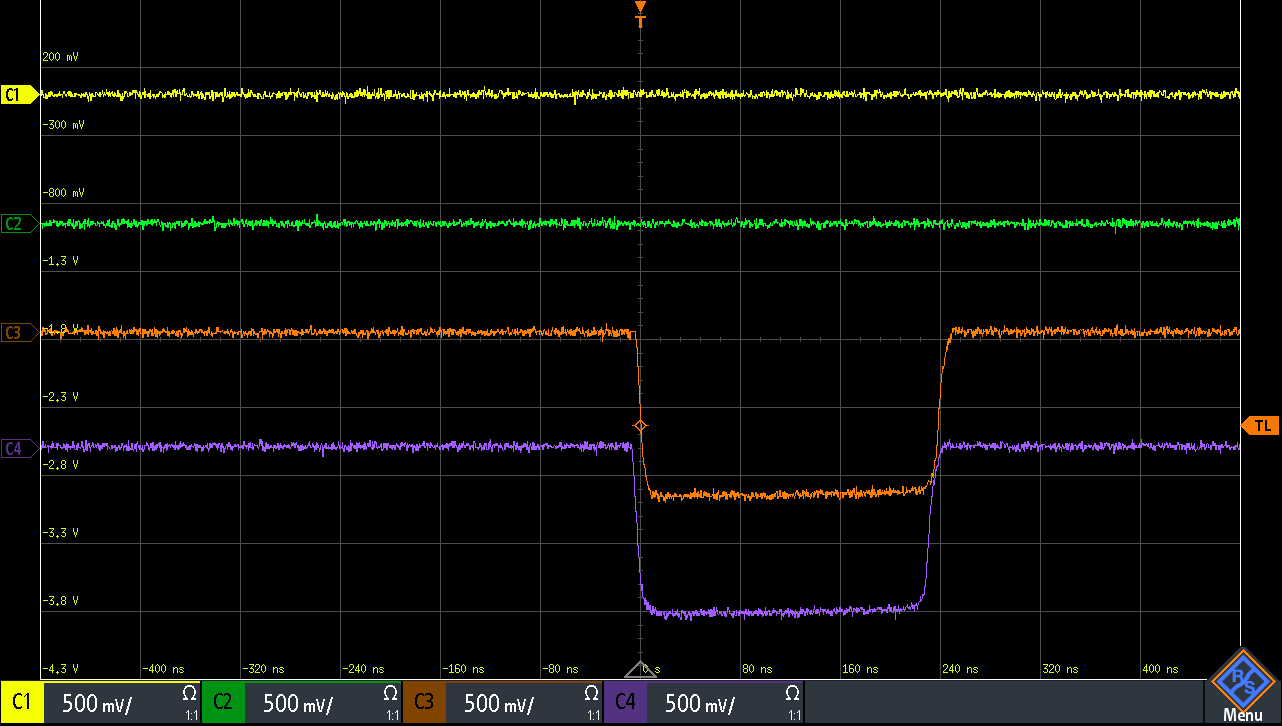
\includegraphics[width=0.5\textwidth]{3DesignPrinciples/32Tritium_detector/2_coincidences_2.png}}
    \subfloat[Event detected in all PMTs, both detector.]{
   \label{subfig:signalInAllPMTsBothDetector}
    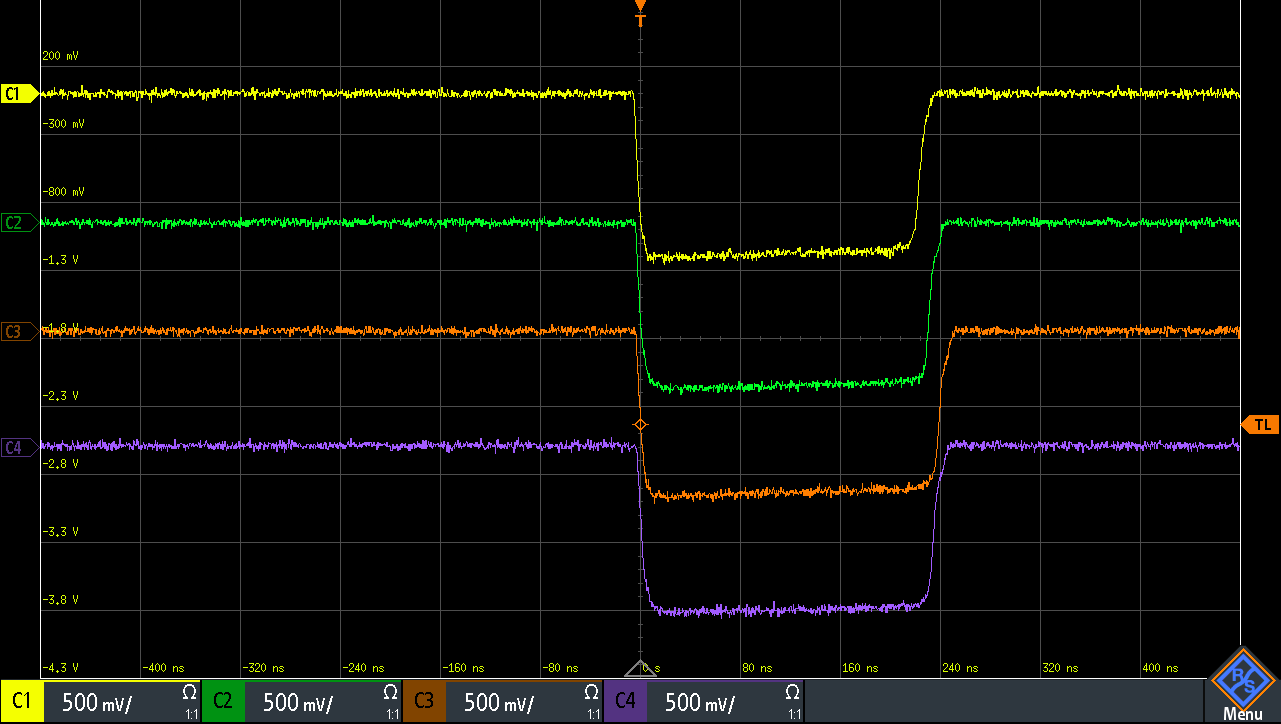
\includegraphics[width=0.5\textwidth]{3DesignPrinciples/32Tritium_detector/4_coincidences.png}}
 \caption{Different situation that can happen when we do time coincidences with PMTs.}
 \label{fig:DifferentCoincidences}
\end{figure}


\end{enumerate}

\item{} Finally, the logical output signal of the coincidence module used, which indicates that all the PMTs used in our study are in temporal coincidence, is introduced in the "Gate and Delay Generator, model 416A" of the company ORTEC \cite{DataSheetGateAndDelay}. With this NIM module we obtain a positive logical signal, shown in the figure \ref{fig:InputSignalsMCA}, orange color, with a height of $8~\volt$ and width of $2~\mu\second$.

\end{enumerate}

\end{itemize}

At the end, we have two different signals, shown in figure \ref{fig:InputSignalsMCA}, which will be introduced in the MCA 8000D, Pocket MCA from AMPTEK company \cite{DataSheetMCA} to be saved. On the one hand we have an analog signal (output from the amplifier module) that has information about the event that has been detected (its energy, detection time, etc.) and this is the signal whose information we will save for analyzing. On the other hand we have a logic signal (output from the Gate and Delay Generator module) that indicates when we have to save the amplified signal, that is, when all our PMTs used in our experiment have detected an event at the same time.

\begin{figure}[htbp]
\centering
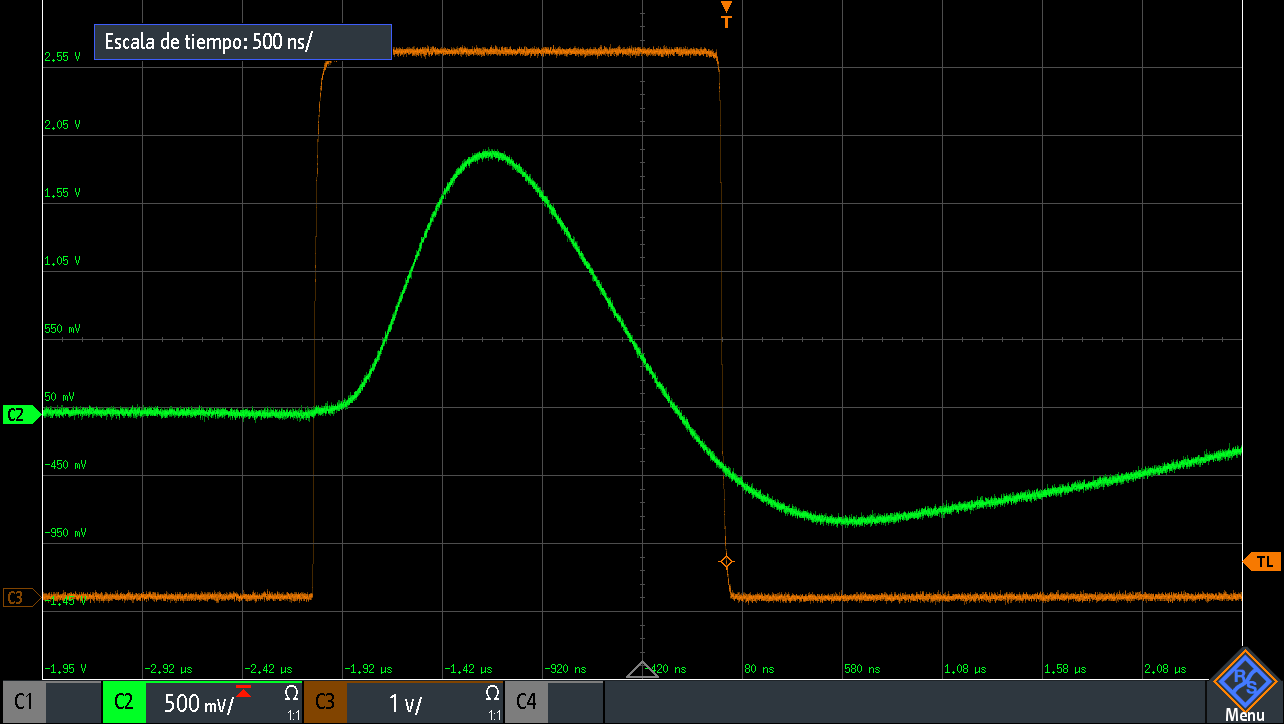
\includegraphics[scale=0.3]{3DesignPrinciples/32Tritium_detector/Input_MCA.png}
\caption{Signal amplificated and logical gate (input signals of MCA).\label{fig:InputSignalsMCA}}
\end{figure}


The information that will be saved and histogramed in the MCA is the weight of the signal, which is proportional to the energy of the detected event, explained in the appendix \ref{App:ElectronicModulesNIM}. An example of histogram as output of the MCA is shown in figure \ref{fig:EnergySpectrum4PMTs}.

\begin{figure}[htbp]
\centering
%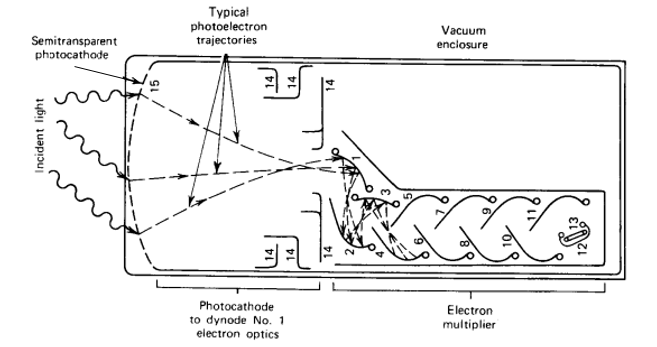
\includegraphics[scale=0.6]{3DesignPrinciples/32Tritium_detector/PMTschematic.png}
\caption{Energy spectrum obtained with the electronic configuration explained in this section for four PMTs.\label{fig:EnergySpectrum4PMTs}}
\end{figure}
\label{subsubsec:PMTsElectronicalSystem}
			%\newpage
			
			\subsubsection[Electronical system for a SiPM]{Electronical system for SiPMs}
			Before talking about the electronic system that is used for reading SiPM, we have to keep in mind that we are using SiPM arrays in TRITIUM detector. The electronic system used to process and analyze these output signals is PETSYS \cite{PETSYS}, which is a commercial system prepared to work with SiPM matrices from Hamamatsu, which is the SiPM company chosen for us.

Petsys system, figure \ref{fig:PETSYS}, is a complete acquisition and digitization system that is capable of working with up to 1024 SiPM arranged in matrices of up to 64 SiPM per matrix. This capacity is necessary because, as we will see in chapter \ref{chap:Prototypes}, TRITIUM monitor will use dozens of SiPM matrices with 16 channels (SiPMs) per matrix.

\begin{figure}[htbp]
\centering
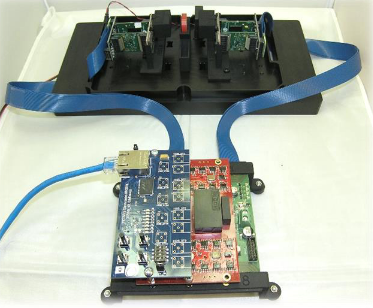
\includegraphics[scale=0.6]{3DesignPrinciples/32Tritium_detector/PETSYS_System.png}
\caption{Different parts of PETSYS system.\label{fig:PETSYS}~\cite{PETSYS}}
\end{figure}

Taking into account the current detection limits imposed, this capacity should be enough for TRITIUM detector but, as we will see in chapter \ref{chap:Prototypes}, TRITIUM is a modular detector. If we need to overcome its limits reached (improve its sensitivity or reduce their background even more) we will need to increase this capacity. We need an electronic system that is able to increase its capacity in a modular way and PETSYS meets this requirement. It has the Clock and Trigger module with which we have the possibility of connecting up to sixteen different PETSYS basic boards in parallel with which we could read up to 16384 SiPM\footnote{$1024\cdot{}16 = 16384$}.

PETSYS is based on C++ and Python scripts that are prepared for the main tasks required for our experiment, such as time coincidence options between SiPM (or even SiPM matrices) or energy discrimination. In addition, PETSYS is open source, so if it is necessary, we have the option to modify the scripts for developing interesting functions. The way the signals will be processed and analyzed for PETSYS will be exactly the same as those shown in the figure \ref{fig:ElectronicConfiguraitonsPMT}

This system has a time resolution of $250~\pico\second$ which is one of the best time resolutions of commercial systems available today and its price is around $10$\euro$/$ channel, which is very cheap in comparison with current similar electronic systems.

As we will see in the section \ref{sec:CharacterizationSiPM}, the temperature of each SiPM matrix is an important parameter to take into account. The PETSYS system has the ability to monitor the temperature of both, the SiPM matrices and ASICS that are used to control them during the measurements.

Although PETSYS is the system used to work with SiPM matrices in the TRITIUM detector, it does not allow characterizing the SiPMs, which is an important task to understand the results of our detector.

In order to do so, we have designed, developed and built an electronic system with which we can read up to eight different SiPMs. With this system we can also monitor the temperature of the SiPMs used.

This system is based on three different PCBs\footnote{PCB, Printed Circuit Board}, which are shown in figure \ref{fig:PCBs_LEDSpectrum} and whose electronical schemes are shown in the appendix \ref{App:ElectronicalSchemesSiPMPCBs}:

\begin{enumerate}
\item{} The first PCB, shown in figure \ref{subfig:PCB1}, is used to organize the SiPMs and sensor temperature in this system. This PCB has the ability to place up to 8 different SiPMs and a temperature sensor and arrange these signals on two HDMI connections.

This PCB will be inside a special black box, from "" company, that has a high degree of light tightness. This black box has a small hole, whose diameter is $1~\mm$, prepared to introduce an optical fiber\footnote{The optical fiber used is BCF-98 from Saint-Gobain company \cite{OpticalFibers}} with which we will illuminate the SiPM with a incoherent light source. The light source used is a LED, model 430L from Thorlabs company \cite{LEDThorlabs}, whose emission spectrum is shown in figure \ref{subfig:LEDSpectrum}, which has been experimentaly measured using a spectrometer and fitted to a Gaussian function. We can see that the emission peak of this LED is produced at $436.3$ with a FWHM\footnote{The FWHM parameter, Full Width at Half Maximum, of a Gaussian fit can be calculated from its sigma using the equation: FWHM$=2.35 \cdot{} \sigma$} of $19.1~\nano\meter$. With this LED we intend to simulate the light emission of the fibers used in the TRITIUM experiment to calibrate the SiPMs at the working wavelength. 

\item{} The second PCB, shown in figure \ref{subfig:PCB2}, is used to sum the different signals from the SiPMs used in the first PCB and amplify the output signal by a factor G. This PCB uses a differential amplification with which we achieve to reduce the electronic noise of the system.

\item{} The third PCB, shown in figure \ref{subfig:PCB3}, is used to arrange all the different input and output signals of this system in an HDMI connection with which we connect to the second PCB. The objective of this PCB is to avoid the introduction of electrical noise by crosstalk between different signals.

The input signals of this system are the supply voltage of the SiPMs and the supply voltage of the PCBs ($\pm 6~\volt$) and the output signals of this system are the temperature sensor signal and the summed signal of all SiPMs. 

\end{enumerate}

\begin{figure}[htbp]
 \centering
  \subfloat[PCB 1 used to arrang 8 SiPMs and black box.]{
   \label{subfig:PCB1}
    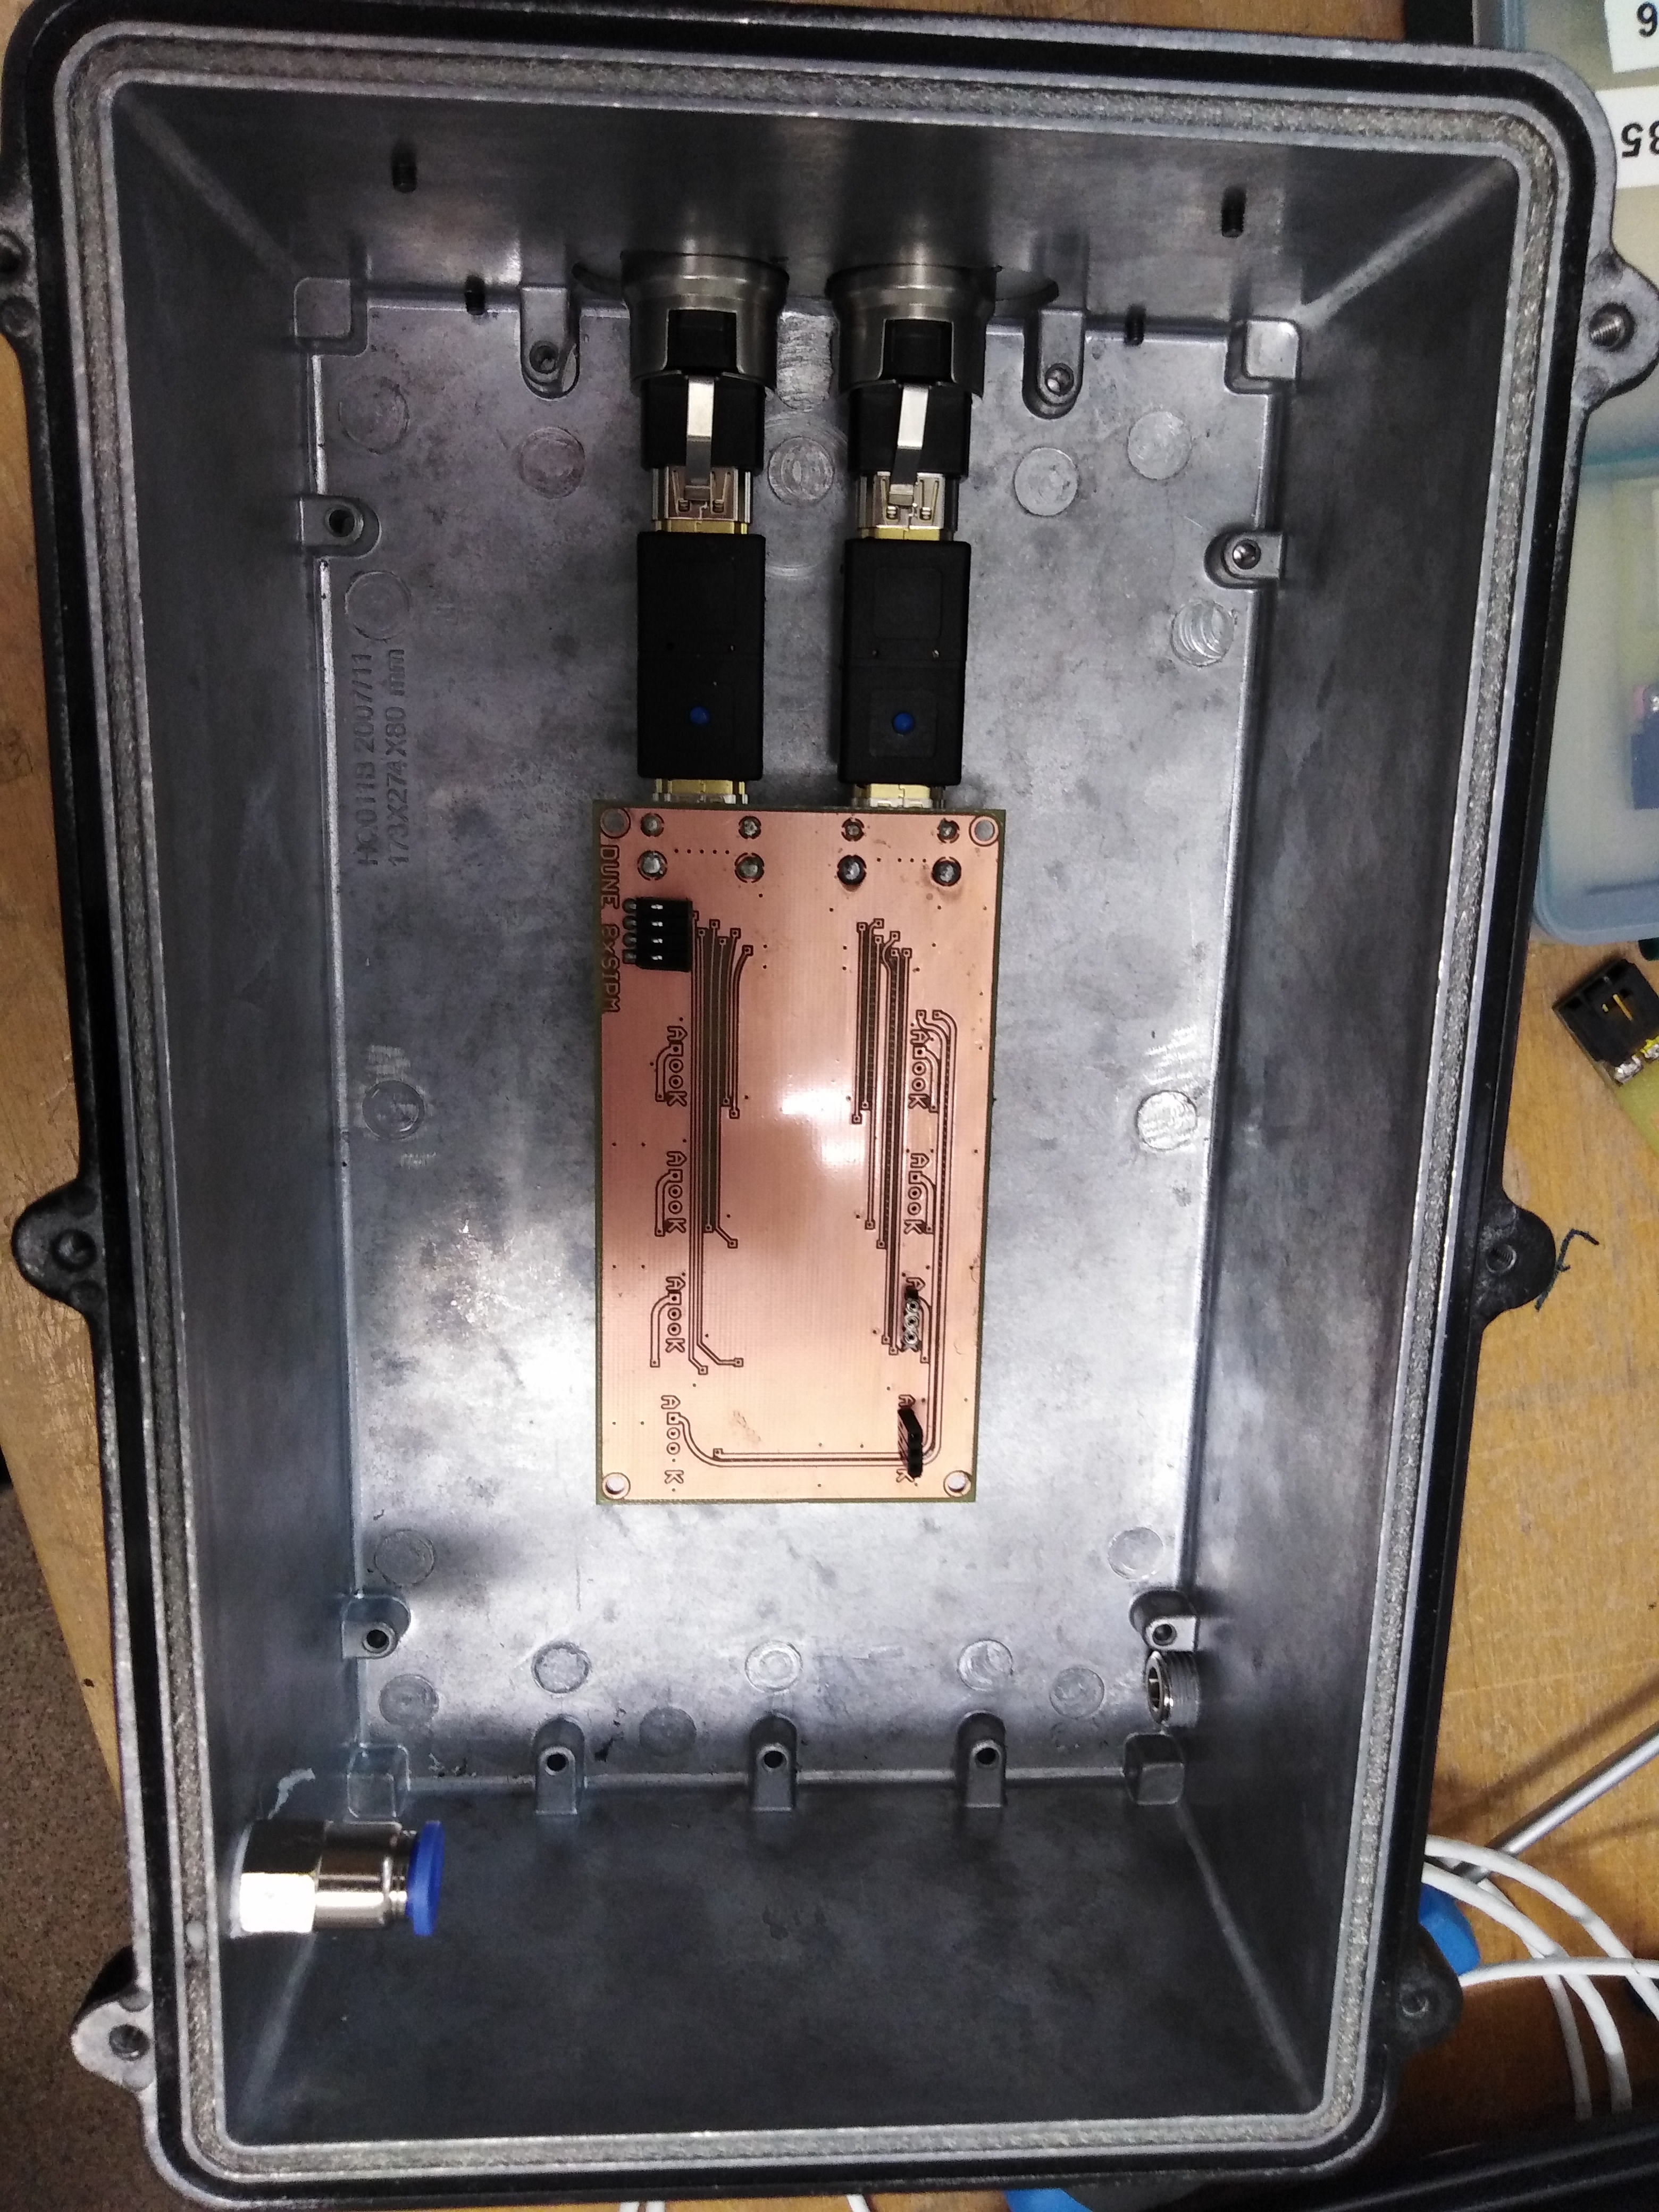
\includegraphics[angle=90,width=0.5\textwidth]{3DesignPrinciples/32Tritium_detector/PCB1_SiPM_Black_Box.jpg}}
  \subfloat[PCB 2 used to sum and amplify the output signals of SiPMs]{
   \label{subfig:PCB2}
    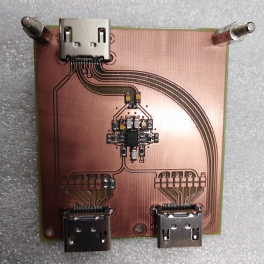
\includegraphics[width=0.45\textwidth]{3DesignPrinciples/32Tritium_detector/PCB2_SIPMs.png}}
   \newline
  \subfloat[PCB 3 used to arrange the different singals of the system.]{
   \label{subfig:PCB3}
    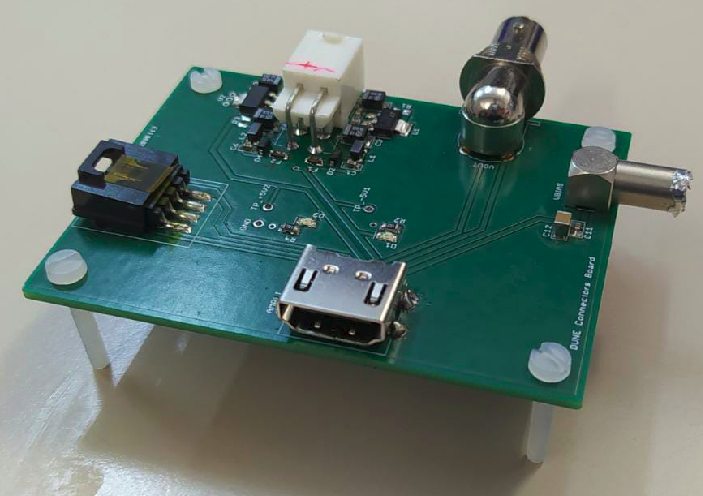
\includegraphics[width=0.4\textwidth]{3DesignPrinciples/32Tritium_detector/PCB3_SiPMs.png}}
    \subfloat[Emission spectrum of the LED.]{
   \label{subfig:LEDSpectrum}
    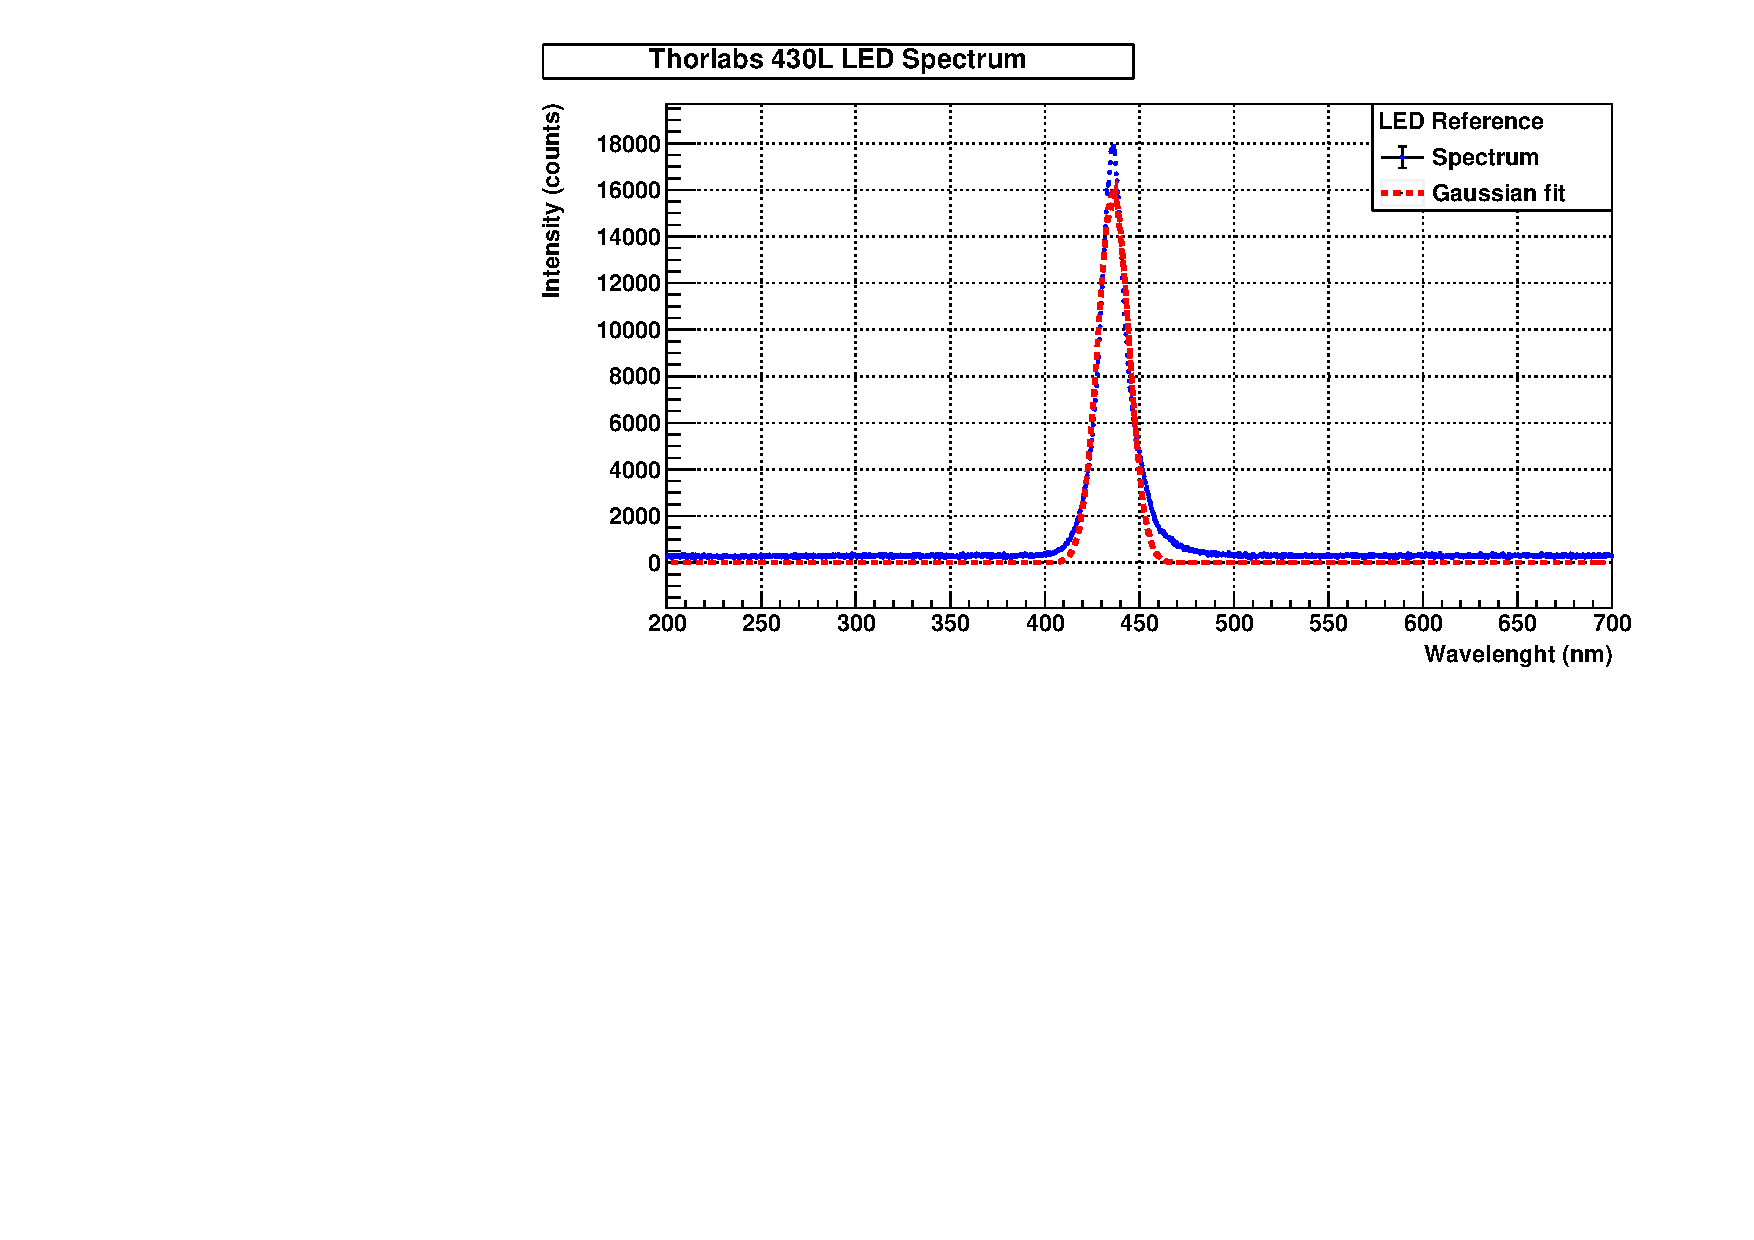
\includegraphics[width=0.6\textwidth]{3DesignPrinciples/32Tritium_detector/LED_DUNE.pdf}}
 \caption{Three PCBs used for the SiPM characterization and LED emission spectrum.}
 \label{fig:PCBs_LEDSpectrum}
\end{figure}\label{subsubsec:SiPMsElectronicalSystem}
			\newpage		
		
	\section{Ultrapure water system}\label{sec:UltraPureWaterSystem}
	%\input{./Sections/2Design_Principles/23UltraPureWaterSystem} 
	%\newpage
		
		\subsection[Introduction water system]{Introduction to the ultrapure water system}
		The aim of using an ultrapure water system is to condition the sample before the measurement. It is important for two reasons:

\begin{itemize}

\item{} On the one hand, it is important because, as we saw in section \ref{sec:TritiumProperties}, the mean free path of tritium electrons in water (our case) is around $5~\mu\meter$ and even less for solid materials like organic material.

For detecting this tritium decay, we need that the electron of its decay reaches the fiber, so we must keep our detector clean. If the analyzed water sample contains particles that can be deposited on the fibers of our detector, it can form a layer of matter, which prevents the tritium electrons from reaching the fibers, reducing the tritium detection efficiency until it becomes impossible to measure tritium.

\item{} On the other hand, we have to keep in mind that, as we will see in chapter \ref{chap:Prototypes}, the tritium monitor does not have any spectrometric capabilities that can be used to distinguish other radioactive elements from tritium. That means that, all the radioactive element included in the analyzed water sample will be computed as a tritium event.

With this system we can remove all particles up to a diameter of $1~\mu\meter$ and organic matter, which means that we remove all particles and molecules other than water. Since tritium is the only radioactive element that can be practically equal to water (when it is in the $\ce{HTO}$ form, the majority form in wihch tritium are present in the water sample), with this process we remove all particles radioactive elements other than tritium and the amount of tritium present in the sample is not affected

\end{itemize} 

In summary, with the ultrapure water system we get to keep our detector clean, ensuring the stability of its detection efficiency and we eliminate all radioactive particles other than tritium, maintaining the activity of the tritium in the sample, so we do not need any spectroscopic capabilities in our detector to distinguish radioactive elements. Both reasons has been tested with experimental measurements that will be shown in the chapter \ref{sec:CharacterizationUltraPureWaterSystem}. \label{subsec:IntroductionWaterSystem}
		%\newpage
					
		\subsection[Set up water system]{Set up of ultrapure water system} %\label{sec:Scintillators}
		The main objectives of this water treatment device are:

\begin{itemize}

\item{} Obtaining a high degree of purification in the processed water sample, reducing its conductivity by approximately two orders of magnitude (from $1000~\mu$S$/\cm$ up to $10~\mu$S$/\cm$)

\item{} Designing of a device with low maintenance (low cost  and low manpower)

\item{} Installation of a remote control devices such as probes and valves and development of a software to management it.
\end{itemize}

For this, the LARUEX laboratory in Extremadura, one of the six collaborators of the TRITIUM experiment, has designed, developed and built an ultrapure water system, whose scheme is shown in figure \ref{fig:WPSScheme}.

\begin{figure}[htbp]
\centering
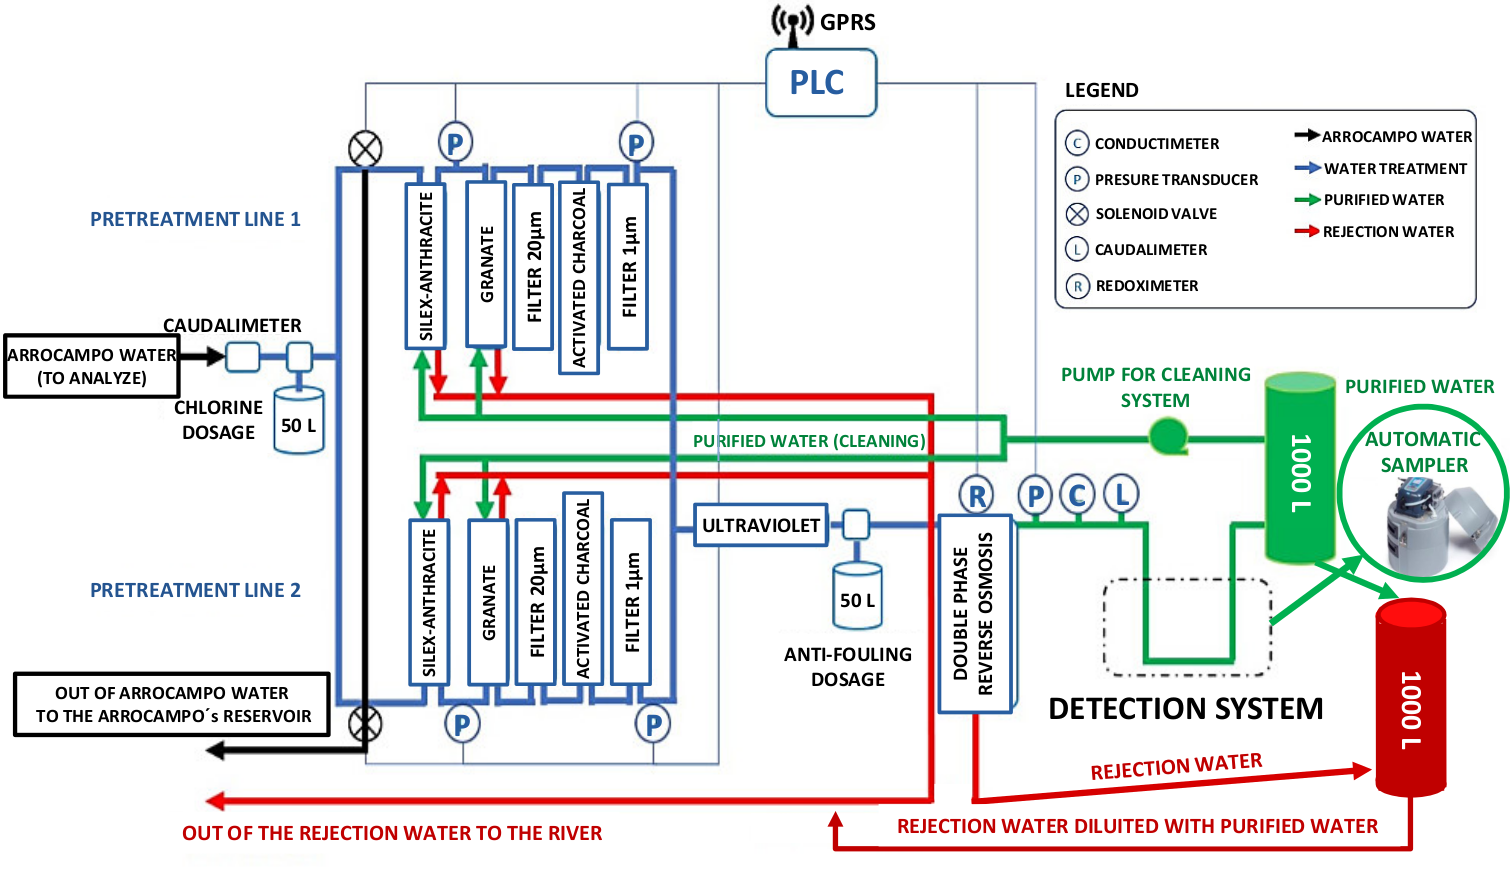
\includegraphics[scale=0.25]{3DesignPrinciples/33UltraPureWaterSystem/SchemeUltraPureWaterSystem.png}
\caption{Scheme of water purification system.\label{fig:WPSScheme}}
\end{figure}

This system has been installed in the Arrocampo dam and consists of four different consecutive stages:

\begin{itemize}
\item{} First, the raw water from the Tagus River is introduced into two different filters, the first formed by Silex-Anthracite and the second by granate, with which we make a gross filtering (the largest particles are eliminated). There are two parallel lines that are capable of self-cleaning by injecting ultrapure water in the opposite direction.

\item{} Next, this water sample is introduced into a $20~\mu\meter$ filter (Formed by a synthetic mesh) and activated charcoal filters (one per line in both) that form the fine filtration stage. With the $20~\mu\meter$ filter we can filter particles with diameters of up to $20\mu\meter$ and, with the activated charcoal filter, we remove the chlorine and iron particles from the sample.

\item{} Then, this water sample is introduced into the super-fine filtering consisting of a $1~\mu\meter$ filter, formed of a dense polypropylene mesh, (one per line), and UV lamps. With the first we remove all the particles up to diameters of $1~\mu\meter$ and, with the second, we remove the organic matter present in the purified water sample.

\item{} Finally, this water sample is introduced in the last stage, double-phase reverse osmosis, thereby reducing the conductivity of the water to values of $5~\mu$S$/\cm$. We verified that we achieve a conductivity of $10~\mu$S$/\cm$ with only one module reverse osmosis and this is enough for the needed conditions of tritium detector. Therefore, we use just one module of reverse osmosis for $24~\hour$ and the other for another $24~\hour$, thereby reducing the power consumption of the system.

\end{itemize}

At the end of this system, each water sample is divided into two different outlet samples. The pure water sample, which is the ultrapure water that will be injected into tritium detector, and the rejection water, whose turbidity is even greater than the water sample before treatment because it contains all the particles that have been extracted from the ultrapure water sample.

With this ultrapure water system we can process up to $0.850~\meter^3/\hour$ with a single line operating or $1.480~\meter^3/\hour$ with both, greatly overestimating the requirements of the tritium detector. 

The software used for remote controlling the ultrapure water system is Siemens PLC, with which we receive information fo this system sush as the state of the valves, the pressure probes or water production in real time. 

Several photos of this system are shown in the appendix \ref{App:UltraPureWaterSystem}.\label{subsec:SetUpWaterSystem}
		\newpage	
	
	\section[Background rejection system]{Background rejection system of TRITIUM monitor}\label{sec:BackgroundShields}
	The objective of this section is to reduce the radioactive background that affects the TRITIUM detector. It is important because we are following the ALARA principle for the tritium activity measurement, that is, to measure tritium activity "as low as reasonably achievable".

We have to take into account that the low limit reached in the tritium activity measured with our detector will be limited due to the uncertainty in the activity of the radioactive background measured since we cannot measure tritium activities lower than this uncertainty. Therefore, if we want to measure tritium activities as low as possible, we must reduce this background uncertainty as much as possible.

The total uncertainty of the measurement is a quadratic sum of all the different uncertainties present in this measurement, which is the statistical uncertainty, $\sigma_{st}$, (due to the statistical nature of the radioactivity process), the systematic uncertainty, $\sigma_{si}$, (due to the manufacture of the detectors), etc (equation \ref{eq:SquareSumUncerainty}).

With the background rejection system of TRITIUM monitor we try to minimize the statistical component. Because of the Poissonian nature of the process, the statistical component of the uncertainty corresponds to the square root of the measured activity, $A_{m}$, equation \ref{eq:SquareSumUncerainty}, so, if we want to reduce this component, we must minimize the radiological background that affects our detector as much as posible.

\begin{equation}
\sigma_{T}^2 = \sigma_{st}^2 +\sigma_{si}^2 + ... ; \qquad \qquad \sigma_{st;bac} = \sqrt{A_{m;bac}}
\label{eq:SquareSumUncerainty}
\end{equation} 

The background that affects the tritium detector is due to natural radioactivity, which is present in all parts of the earth and it has two main origins. On the one hand, it can come from radioactive elements of the natural radioactive series, shown in table \ref{tab:NaturalRadioactiveSeries}, which are the primordial radioactive elements, those that are present since the formation of the earth. On the other hand, it can come from natural radiation received from extraterrestrial sources, called cosmic radiation, composed of high-energy particles, mainly protons and $\alpha$, which, when they interact with the particles in the Earth's atmosphere, generate a shower of muons, photons and neutrons mainly.

\begin{table}[htbp]
%%\centering
\begin{center}
\begin{tabular}{|c|c|c|c|c|}
\hline
Mass Num. & Series & Prim. el. & Half life (y) & Final isotope \\
\hline \hline \hline
4n & Thorium & $\ce{^{232}Th}$ & $1.41 \cdot{} 10^{10}$ & $\ce{^{208}Pb}$ \\ \hline
4n+1 & Neptunium & $\ce{^{237}Np}$ & $2.14 \cdot{} 10^{6}$ & $\ce{^{209}Pb}$ \\ \hline
4n+2 & Uranium-Radium & $\ce{^{238}U}$ & $4.51 \cdot{} 10^{9}$ & $\ce{^{206}Pb}$ \\ \hline
4n+3 & Uranium-Actinium & $\ce{^{235}U}$ & $7.18 \cdot{} 10^{8}$ & $\ce{^{204}Pb}$ \\ \hline
\end{tabular}
\caption{Classification of natural radioactive series.\cite{}}
\label{tab:NaturalRadioactiveSeries}
\end{center}
\end{table}

Natural radioactivity depends on the altitude and latitude at which we are on Earth because the volume of the Earth's atmosphere, with which cosmic rays interact, is different. For the same reason, it also depends on the height at which we are working, at sea level in our case, and, due to the relative position of the earth in the universe, it also depend on the solar activity cycle in which we are when we measure. The spatial distribution of cosmic rays, mainly muons, follows a $cos^2(\theta)$ distribution with the zenith angle. %In any case, we have to keep in mind that we will be located in the same place when we work, the Arrocampo dam, so we do not need to take it into account.

We will divide this natural radioactivity into two parts and we will use a different technique to prevent these events from affecting the tritium measurement:

\begin{itemize}

\item{}  On the one hand, we have weak radiation, which is any radiation whose energy emission is below $200~\MeV/$nucleon. To avoid that these events affect the tritium measurement, we will use a lead shield, explained in the section \ref{subsec:SetUpPassiveShield}, with which we stop this radiation before it reaches the tritium detector.

\item{} On the other hand, we have the hard radiation, that is, any radiation whose energy emission is greater than $200~\MeV/$nucleon (mainly cosmic radiation). We have to keep in mind that it is much more difficult to stop hard radiation than weak radiation, so instead of stopping this radiation, what we will do is to build an active veto, which are explained in the section \ref{subsec:SetUpActiveShield}, with which we only detect a hard cosmic event and it will be used in anti-coincidence with the TRITIUM detector, that is, we will save the measured tritium event just when we don't measure any hard cosmic event in time coincidence.

\end{itemize} \label{sec:IntroductionBackground}
	%\newpage
	
		\subsection[Set up passive shield]{Set up of the passive shield (lead)} %\label{sec:Scintillators}
		To stop the weak radiation we use the so-called passive veto, which consists of a lead shielding inside which we will place the TRITIUM detector. This lead shielding is used to stop external particles before they reach the tritium detector, affecting the tritium measurement. It will work for particle energies below $200~\MeV/$nucleon, which is mainly the earth's natural radioactivity and the weak component of cosmic radiation.

This lead shielding consists of $158$ lead bricks with ultra-low instrinsec radioactivity, $A \approx NUMBER$. The thickness of this bricks are $25~\mm$ and they are shaped like a shevron, shown in the figure \ref{subfig:LeadBricks}, specially designed for a perfect fit and easy assembly. As can be seen in the figures \ref{subfig:TwoLayers} and \ref{subfig:TwoLayers2}, these lead bricks are arranged in two layers leaving a total thickness of the lead shielding walls of $50~\mm$ and the space between the lead bricks in the inner layer is overlaid with a lead brick of the outer layer to avoid possible entry of radiation.

\begin{figure}[htbp]
 \centering
  \subfloat[Lead bricks.]{
   \label{subfig:LeadBricks}
    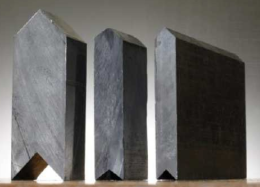
\includegraphics[width=0.3\textwidth]{3DesignPrinciples/34BackgroundRejectionSystem/LeadBricks.png}}
  \subfloat[Two layers for the lead bricks of the shielding.]{
   \label{subfig:TwoLayers}
    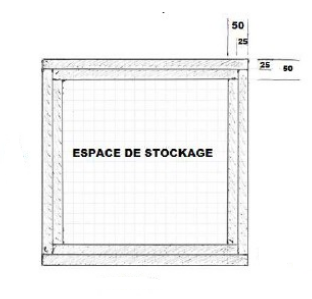
\includegraphics[width=0.3\textwidth]{3DesignPrinciples/34BackgroundRejectionSystem/TwoLayers.png}}
   %\newline
  \subfloat[Two layers for the lead bricks of the shielding.]{
   \label{subfig:TwoLayers2}
    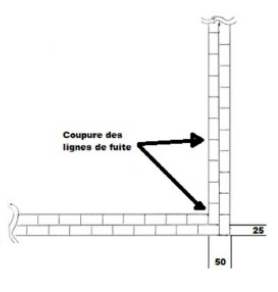
\includegraphics[width=0.3\textwidth]{3DesignPrinciples/34BackgroundRejectionSystem/TwoLayers2.png}}
 \caption{Lead Bricks and their arrangement in the lead shielding.}
 \label{fig:LeadBricksAndArrangement}
\end{figure}

Mechanical engineering department of CENBG has designed a special aluminum structure, shown in figure \ref{fig:AluminiumStructure}, to support the total weight of the lead bricks, $2.4$ tons.

\begin{figure}[htbp]
 \centering
  \subfloat[Aluminium structure scheme.]{
   \label{subfig:AluminiumStructureScheme}
    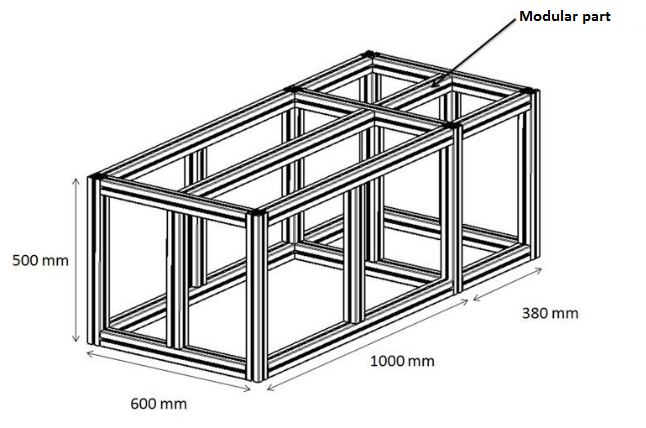
\includegraphics[width=0.45\textwidth]{3DesignPrinciples/34BackgroundRejectionSystem/AluminiumStructureScheme.png}}
  \subfloat[Aluminium structure of TRITIUM monitor.]{
   \label{subfig:AluminiumStructure}
    \includegraphics[width=0.4\textwidth]{3DesignPrinciples/34BackgroundRejectionSystem/AluminiumStructure.jpg}}
    \caption{Lead Bricks and their arrangement in the lead shielding.}
 \label{fig:AluminiumStructure}
\end{figure}

The internal space of this lead shielding is arranged in two parts, shown in figure \ref{fig:LeadBricksAndArrangement}. The one, larger, has an internal dimensions of $90.5~\cm$ long, $41~\cm$ deep, and $51~\cm$ high and it will be used to place the TRITIUM detector. The other, smaller, has an internal dimensions of $33~\cm$ long, $41~\cm$ deep, and $51~\cm$ high and it will serve to place the electronic system necessary to collect and store data. The external dimensions of this lead shielding are $148~\cm$ long, $60~\cm$ deep and $70~\cm$ high and a weight of $2.5$ tons.

\label{subsec:SetUpPassiveShield}
		%\newpage
		
		\subsection[Set up Active veto]{Set up of the active shield (cosmic veto)} %\label{sec:Scintillators}
		For this section we have to take into account that the mean free path of particles is proportional to their energy. Therefore, we would need too thick walls to build a lead shield that would be able to stop hard radiation. Instead of trying to stop it, we have used the so-called active vetos.

The active veto consists of several complementary detectors, called cosmic detectors, two complementary detectors for each active veto in our case, with which the hard cosmic events that affect the tritium measurement will be detected and subtracted from the tritium measurement.

As you can see in the figure \ref{fig:VetoAndPrototype}, the way we have done it is to place two complementary detectors, one above the TRITIUM detector and the other below it. 

\begin{figure}[]
\centering
\includegraphics[scale=0.45]{3DesignPrinciples/34BackgroundRejectionSystem/Vetos_y_prototipo.png}
\caption{Active veto and Tritium-IFIC 2 prototype in an aluminum mechanical structure developed by IFIC's mechanical engineering department.\label{fig:VetoAndPrototype}}
\end{figure}

We must keep in mind that we only want to eliminate the hard cosmic events that affect the tritium measurement. For that we must take into account that this active veto must be placed within the lead shielding. This is because, in this case, the weak radiation, which can contribute as a false hard comic events, has been removed.

Each cosmic detector will have two photosensors, four photosensors in each active veto. The most likely hard cosmic events that can affect the tritium measurement will pass through both cosmic detectors at the same time. To eliminate only them, the first thing we will do is detect only these hard cosmic events, which is achieved by reading both cosmic detectors in coincidence with the electron configuration shown in figure \ref{subfig:ElectronicConfiguraiton4PMT} and then we will read the TRITIUM detector in anti-coincidence with the active veto, that is, store the tritium measurement only when we don't detecte any hard cosmic event in the active veto. 

In this case, if we have detect a hard cosmic event (time coincidence event in both cosmic detectors), we can be quite sure that it will cross through the tritium detector and, therefore, it will affect to their measurement, as you can see in the figure \ref{subfig:RealHardCosmicEvent}.

There is a possibility that this hard cosmic event detected in the active veto comes from two different hard cosmic events (one detected in each cosmic detector as shown in figure \ref{subfig:FakeHardCosmicEvent} but, if we take into account the hard cosmic distribution, shown in figure \ref{subfig:HardCoscmicRate}, we can see that this probability is practically negligible.

The hard cosmic events expected at sea level are of the order of $10^{-2}~$event$/\second/\cm^2$. If we take into account that we are doing time coincidences with signals whose width is of the order of $10~\nano\second$ we can see that the probability of obtaining two different hard cosmic events in temporal coincidence is less than $10^{-9}$ which is practically insignificant so they are not worth considering.

\begin{figure}[]
 \centering
  \subfloat[Real hard cosmic event.]{
   \label{subfig:RealHardCosmicEvent}
    \includegraphics[width=0.25\textwidth]{3DesignPrinciples/34BackgroundRejectionSystem/Real_Event.png}}    
  \subfloat[Fake hard cosmic event.]{
   \label{subfig:FakeHardCosmicEvent}
    \includegraphics[width=0.25\textwidth]{3DesignPrinciples/34BackgroundRejectionSystem/Fake_Event.png}} 
    \subfloat[Hard cosmic rate.]{
   \label{subfig:HardCoscmicRate}
    \includegraphics[width=0.42\textwidth]{3DesignPrinciples/34BackgroundRejectionSystem/HardCosmicRate.png}}     
 \caption{Hard cosmic events detected with the active veto of TRITIUM: a) Affecting to the tritium measurement, b) Does not affecting to the tritium measurement. c) Hard cosmic rate.}
 \label{fig:HardCosmicEventsSimulation}
\end{figure}

Finally, these individual cosmic detectors, on which the active veto is based, consist of a plastic scintillator block from Epic-Crystal \cite{ScintillatorVeto}, whose properties and energy emission spectrum are shown in table \ref{tab:ParametersScintillatorVeto} and figure \ref{fig:EmissionEnergySpectrumVeto} respectively.

\begin{table}[htbp]
%%\centering
\begin{center}
\begin{tabular}{|c|c|c|}
%\hline
%Material & Refractive index \\
\hline \hline 
Base material & Polystyrene \\ \hline
Growth method & Polymeric \\ \hline
Density ($\gram/\cm^3$)& 1.05 \\ \hline
Refractive index & 1.58 \\ \hline
Soften temperature ($\degree$) & 75-80 \\ \hline
Light output (Anthracene) & 50-60\% \\ \hline
H/C raito & 1.1 \\ \hline
Emission peak (nm) & 415 (Blue) \\ \hline
Decay Time, (ns) & 2.4 \\ \hline
Hygroscopic & No \\ \hline
\end{tabular}
\caption{Properties of plastic scintillator blocks from Epic-Crystals. \cite{ScintillatorVeto}}
\label{tab:ParametersScintillatorVeto}
\end{center}
\end{table}

\begin{figure}[]
\centering
\includegraphics[scale=0.45]{3DesignPrinciples/34BackgroundRejectionSystem/EmissionEnergySpectrumVetos.png}
\caption{Emission energy spectrum of the plastic scintillation used for the active vetos.\label{fig:EmissionEnergySpectrumVeto}~\cite{ScintillatorVeto}}
\end{figure}

The dimensions used are $45~\cm$ long, $17~\cm$ deep and $1~\cm$ of thickness and they are covered by three layers, teflon, aluminum and black tape, shown in figure \ref{fig:LayersVeto}, which is used, on the one hand, to prevent external photons from reaching the scintillator plastic, giving false hard cosmic events and, on the other hand, to prevent the photons generated by the scintillator plastic from escaping before reaching the photosensor, losing real hard cosmic events.

\begin{figure}[]
 \centering
  \subfloat[Scintillator without coating.]{
   \label{subfig:PlasticScintillatorNoCoating}
    \includegraphics[width=0.23\textwidth]{3DesignPrinciples/34BackgroundRejectionSystem/NoCoating.jpeg}}    
  \subfloat[Teflon coating.]{
   \label{subfig:PlasticScintillatorTeflon}
    \includegraphics[width=0.23\textwidth]{3DesignPrinciples/34BackgroundRejectionSystem/TeflonCoating.jpeg}}  
  \subfloat[Aluminium coating.]{
   \label{subfig:PlasticScintillatorAluminium}
    \includegraphics[width=0.23\textwidth]{3DesignPrinciples/34BackgroundRejectionSystem/AluminiumCoating.jpeg}}    
  \subfloat[Black tape coating.]{
   \label{subfig:PlasticScintillatorBlackTape}
    \includegraphics[width=0.23\textwidth]{3DesignPrinciples/34BackgroundRejectionSystem/BlackTapeCoating.jpeg}}
 \caption{Different layers used to cover of the active veto.}
 \label{fig:LayersVeto}
\end{figure}

This coating has two windows where we can place both photosensorsto read the photons produced by the plastic scintillator.

For TRITIUM active vetos we should expect a rate of $1$ events$/\second$ for hard cosmic events. This value has been calculated integrating the previously mentioned value, $10^{-2}~$event$/\second/\cm^2$, over the area of the TRITIUM active vetos. For our specifically case, we can check that the probability of obtaining two different hard cosmic events in temporal coincidence is $10^{-7}$ and it remain insignificant.\label{subsec:SetUpActiveShield}
		\newpage
					
\chapter[Research \& Development]{Research \& Development on detector design and components}\label{chap:ResearchandDevelopment}
	\section{Introduction (why is important)}
	This chapter shows the characterization of each individual part of the TRITIUM monitor, which includes scintillating fibers, SiPMs (at the individual SiPM level and at the matrix level), the ultrapure water system and the background rejection system, consisting of the lead shielding and the active veto. 

This characterization is one of the most important things to do because it will help us to understand their behaviour and the results obtained with the complete monitor. Furthermore, we have made some developments to improve interesting parameters of the TRITIUM monitor components to enhance the monitor's capabilities for tritium detection.

All these studies have been carried out inside a special light-tight black box to ensure that the photons we are detecting come from the photon sources used, whether they are emitted by LEDs or by scintillators. Furthermore, because of the reason that we cannot do an accurate energy calibration when using plastic scintillators, we will show some energy spectrums in units of channels (units of ADC), which are linearly proportional to the units of energy. \label{sec:IntroCharacterisation}
	\newpage
	
	\section[Characetrization fibers]{Characterization and R\&D on scintillating fibers}
	\input{./Sections/3ResearchAndDevelopment/32CharacterizationFibers}\label{sec:CharacterizationScintillatingFibers}
	\newpage
		
	\section[Characterization SiPM]{Characterization and R\&D on SiPM}
	This section describe the work that has been carried out to characterize the SiPMs used in the TRITIUM experiment, model S13360-6075 from Hammamtsu Photonics company. It will consist of measuring some of the most important parameters of this SiPM that will affect the tritium measurement such us their break down voltage or their gain.

Furthermore, a temperature compensation method has been developed and experimentally tested to compensate for temperature variations of the SiPM since it has been seen to greatly affect to its correct operation and, therefore, the measurement of tritium.

The setup used in this characterization is shown in section \ref{subsubsec:SiPMsElectronicalSystem}, figure \ref{fig:PCBs_LEDSpectrum}. Furthermore, these measurements were performed inside of a climatic chamber whose temperature and humidity were controled with a precision of $0.1~\degree$ and $0.1\%$ respectively. We have to take into account, when the system was stabilized, variations with the same size of this precision were observed.

First of all we measured to breakdown voltage of the SiPM and their quenching resistance which was calculed from the measurement of their current-voltage curves. To measure it we need to work without amplification of the electronic system so, insatead to use the second and third PCB, we connected the output of the black box directly to the picoammeter, whose reference has been given in the \ref{} section. A LabView program was used to automate the taking of measurements.

On the one hand, we feed the SiPM using a forward bias voltage from $0~\volt$ to $1.58~\volt$ in steps of $0.005~\volt$, whose result is shown in figure \ref{}.

FIGURAAA

EXPLICACIOON

On the other hand, we feed the SiPM using the reverse bias voltage...



the black box output was connected directly to the keithley to measure the current and using

This calibration will consist of two different parts. On the one hand, we measure the IV curves of the SiPM, from which we will calculate the breakdown voltage and the quenching resistance of the SiPM and, on the other hand, we will measure energy spectrums from which we will calculate the gain of the SiPM, the equivalent capacity of the SiPM, etc.

To measure the energy spectrums we will use the setup shown in section \ref{} and to measure the IV curves a small modification of this setup will be made which consists of... 




Pequeñas zonas de deplexión crean grandes capacidades que producen alto ruido de los SiPMs

Trabajo de Fernando Hueso.

Explicar electrónica que se utiliza como la tarjeta y demas. Poner el esquema electrónico de la tarjeta y referencia a Marc de NEXT por haberla construido. Explicar la forma del pulso como en la tesis de Karina Asnar

Paper de Nadia para la PDE.

Las medidas se han hecho en la camara del IFIMED (ver lo que tengo apuntado en el TFM y dar gracias al IFIMED)

la banda prohibida es pequeña por lo que algunos electrones pueden excitarse termicamente y pasar a la banda de conducción -> RUIDO
Cuando hable del ruido, afterpulses, crosstalk... intro en MPPC hammatsu data sheet

cuando hable de la capacidad del SiPM utilizar el punto 10.3.2 del Leo -> pag. 226

resumen de como varía cada magnitud con la temperatura y el voltaje. Tesis SiPMs.

Inocherent light source!

fired cells.


paper NADIA

B. Photon Detection Efficiency -> entero.

Aunque el aumentar el voltaje inverso mejora la eficiencia de detección de fotones, también aumenta la corriente oscura. Reducir la temperatura sin embargo disminuye la corriente oscura.

Para contar el número de veces que dos o más fotones son detectados simultáneamente, el umbral les establecido en N – 0.5 p.e. (donde N es un número arbitrario de fotones). Al contar el número de pulsos que exceden este umbral se puede saber el número de veces que se han detectado simultáneamente N o más fotones (Manual Hamamatsu, 2008, 2007)

En este trabajo se estudió tanto la variación en la resolución en energía de un SiPM como la variación del centroide de un pico (explicado a detalle en los próximos capítulos) con la temperatura y el voltaje. Para ello se estableció una electrónica de adquisición adecuada para la mayor eliminación de ruido posible y óptima resolución (explicada en el Capítulo 3).


Superponer 2 plots con el LED a distintos voltajes (2 o mas... probar varios voltajes a Vov recomendado y quedarnos con los mejores).

Figura 11 de la tesis de cristales monoliticos

La ganancia M, depende exponencialmente de la tensión de polarización inversa del dispositivo (Fig. 11, derecha). Sin embargo, en la región de operación de los APDs con M ~ 100, un cambio relativo de tensión de polarización corresponde a un cambio lineal en la ganancia, con pendientes típicas de 10 \%/V. Además, la temperatura debe estar debidamente estabilizada en un sistema con APDs ya que estos detectores sufren variaciones importantes con la temperatura, típicamente ~ 2-3 \%/ oC

Todo el apartado de SiPMs de esta tesis.

Cuando hablemos del PDE:
El número de celdas de un SiPM dependerá de la aplicación específica. Será lo suficientemente elevado para detectar la cantidad de fotones esperada pero sin exceder innecesariamente este valor, ya que cada celda necesita de espacio para las resistencias de quenching de cada APD y para la separación y aislamiento entre las diferentes celdas. Cuanto mayor sea el número de celdas, mayor será el espacio muerto y menor su eficiencia. Por el contrario, un número de celdas inferior con celdas de mayor tamaño, implica una alta eficiencia de detección de fotones (Photon Detection efficiency, PDE) pero un rango dinámico bajo. La PDE en un SiPM se define como su eficiencia cuántica por el ratio entre el área sensitiva y el área total del dispositivo, lo que se conoce como factor de llenado (fill factor) y se representa con “epsilon”, por la probabilidad de que un fotoelectrón comience un proceso de avalancha (Ec. 19). Aparte de la longitud de onda, 

Este parrafo justirca porque me quedo con el SiPM array de area de SiPM mayor... debido a la sensibilidad... punto 4.2 de la tesis de SiPM (LARGA)



the noise level scales with the area of the device. 




If each ionization process could be considered independent of the others, the fluctuations would then be described by a Poisson distribution where the variance (sigma 2 ) would be equal to the mean number of ionization electrons, N I . However, the fluctuations in the mean number of ionization electrons present a lower value, as predicted by Fano’s theory [66], being proportional to a factor F, known as the Fano Factor, which multiplies the mean primary ionization yield. 


Tiene un factor de amplificación interno que depende exclusivamente de las características de la union p-n y de la resistencia quenching\label{sec:CharacterizationSiPM}
	\newpage
	
	\section[Characetrization water system]{Characterization and R\&D on ultrapure water system}
	Llegamos al nivel de pureza del agua adecuado? Esto daña las fibras? Se reduce la actividad de tritio? \label{sec:CharacterizationUltraPureWaterSystem}
	\newpage
		
	\section[Characterization shields]{Characterization and R\&D on background shields}
	Finally, this section shows the characterization of the active shield (cosmic veto), whose physical configuration has been explained in section \ref{subsec:SetUpActiveShield}. This characterization has been carried out using PMTs as photosensors as shown in figure \ref{fig:VetoAndPrototype}, which are readout using the electronic configuration shown in figure \ref{subfig:ElectronicConfiguraiton4PMT}. Their replacement by SiPMs will be a future study to quantify its improvement to the tritium measurment. 

First of all, we have to find the conditions in which the detection of cosmic events will be optimized by our active veto. It consists of, on the one hand, finding the minimum high voltage of PMTs in which their efficiency is stable, and, on the other hand, finding the maximum threshold of the discriminator, which has to be overcomed by the output signals of the PMTs to contribute to the cosmic detection, at which we start to loss cosmic events in their detection. For higher high voltage and smaller thresholds of the found values, a plateau should be found.

To find both parameters, several measures of the number of coincident events (cosmic events) were done. On the one hand it was measured at several high voltages and fixed thresholds and on the other hand it was measured at several thresholds and fixed high voltages. Both measurements are shown in figure \ref{fig:HVandThresholdsPLateaus} in which a semi-logarithmic scale has been used.

A modification of the electron configuration has been made only for finding these optimal conditions, which consists of using the electronic configuration shown in figure \ref{subfig:ElectronicConfiguraiton4PMT} where the amplification part has been eliminated and the output signal of the coincidence module, second stage, is connected to a HOW IS IT CALLED?? REFERENCE, which is used to count the number of events in a time window ($300$ seconds in our case).

\begin{figure}[]
 \centering
  \subfloat[Counts per second for several high voltage at three different thresholds.]{
   \label{subfig:HVPLateauVetos}
    \includegraphics[width=0.8\textwidth]{4ResearchAndDevelopments/43CosmicVetos/Counts_for_several_HV_VETOS.pdf}}
    \newline
  \subfloat[Counts per second for several thresholds at three different high voltage.]{
   \label{subfig:ThresholdsPlateau}
    \includegraphics[width=0.8\textwidth]{4ResearchAndDevelopments/43CosmicVetos/Counts_for_several_thresholds_VETOS.pdf}}
 \caption{Counts per second at several high voltage and fixed thresholds and several thresholds and fixed high voltage.}
 \label{fig:HVandThresholdsPLateaus}
\end{figure}

In the figure \ref{subfig:HVPLateauVetos}, the measurements at several high voltage and a fixed thresholds is shown, which have been done for three different thresholds, $60~\milli\volt$, $100~\milli\volt$ and $200~\milli\volt$. As can be seen, there is a minimum high voltage for each threshold used, $700~\volt$, $730~\volt$ and $780~\volt$ respectively, at which the plateau start. As we can see this minimum voltage is higher when we increase the value of the threshold, as we should hope. The voltage chosen to work is $800~\volt$ since we can be sure of being on the plateau for the three thresholds.

In the same way, in the figure \ref{subfig:ThresholdsPlateau}, the measurements at several thresholds and a fixed high voltage is shown, which have been done for three different high voltages, $750~\volt$, $800~\volt$ and $850~\volt$. As can be seen, there is a maximum threshold for each high voltage used,  $140~\milli\volt$, $270~\milli\volt$ and $450~\milli\volt$ respectively, at which the plateau ends. Now, we can see that this maximum threshold is increased for higher voltage, as we should hope. The threshold choosen to work is $200~\milli\volt$ since, for our last election $800~\volt$, we can be sure of being on the plateau. 

Next, the energy spectrum of cosmic events was measured, which is shown in figure \ref{fig:EnergySpectrumCosmicVeto}. For this task the electronic configuration shown in figure \ref{subfig:ElectronicConfiguraiton4PMT} was used with the values previously mentioned, $800~\volt$ and $200~\milli\volt$. 

\begin{figure}[h]
\centering
\includegraphics[scale=0.6]{4ResearchAndDevelopments/43CosmicVetos/Cosmic_Energy_Spectrum_36_cm_Landau_Function.pdf}
\caption{Energy spectrum measured with the cosmic veto.\label{fig:EnergySpectrumCosmicVeto}}
\end{figure}

As we can see, this energy spectrum fits well with a landau function as expected. Now, the number of detected cosmic events can be known by calculating the area integral of this spectrum, whose result is $2,5~$event$/\second$. The theoretically expected cosmic rate was calculated in the section \ref{subsec:SetUpActiveShield} for our cosmic vetos, $2,909~$event$/\second$, so the efficiency of it for cosmic events can be calculated, whose value is $85\%$, which is a common value of the efficiency of this type of detectors.

Finally the relationship between the detected cosmic events and the distance between both detectors that form the cosmic veto was obtained. It is interesting because this distance can be changed if other tritium prototypes are used and we need to know the expected cosmic rate for each different situation.

To do so, an energy spectrum was measured for five different distances, $10.4~\cm$, $20~\cm$, $36~\cm$, $39.8~\cm$ and $50~\cm$, which is shown in figure \ref{fig:EnergySpectrumsSeveralDistanceVeto}. The energy spectrum previously shown in figure \ref{} was also included. 

\begin{figure}[h]
\centering
\includegraphics[scale=0.6]{4ResearchAndDevelopments/43CosmicVetos/Energy_Plots_SeveralDistance_Veto.pdf}
\caption{Energy spectrum of cosmic vetos for several distance between cosmic detectors.\label{fig:EnergySpectrumsSeveralDistanceVeto}}
\end{figure}

As we can see, the shape of the spectrum is the same because the energy of the detected events is the same (cosmic events) but the quantity of their events is less for greater distance. The reason for that is that when we increase the distance, the solid angle formed by the active veto is smaller.

The detected cosmic events was calculated by the area integral and they are represented in the figure \ref{fig:LinearFitSeveralDistanceVeto} where a linear fit has been added. With this linear fit, the detected cosmic rate can be easily known whatever the working distance. 

\begin{figure}[h]
\centering
\includegraphics[scale=0.6]{4ResearchAndDevelopments/43CosmicVetos/LinearFit_SeveralDistance_Veto.pdf}
\caption{Linear fit of the counts per second measured with the cosmic veto with several distance between its cosmic detectors.\label{fig:LinearFitSeveralDistanceVeto}}
\end{figure}





También se realizaron varias medias para ver como afecta una fuente gama. Discutir con Pepe como plantear esta medida o si merece la pena ponerla o no.

Como es de esperar esta deja muy poca señal en el centelleador ya que este tiene muy poca eficiencia para gammas.\label{sec:RyDBackground}
	%\newpage
	
	\subsection{Passive shield (lead)}
	\input{./Sections/3ResearchAndDevelopment/35CharacterizationBackgroundShields/352CharacterizationPassiveShield} \label{subsec:CharacterizationPassiveShield}
	%\newpage
					 
	\subsection{Active shield (cosmic veto)} %\label{sec:Scintillators}
	Primero mostrar el espectro energético de antes y despues de recubrir el veto

A continuación mostrar los plateaus de HV y Thresholds.

Luego mostrar el mapeo realizado sobre el veto.

Mirar información sacada por Ana

Presentar la relación cuentas/segundo frente a distancia entre vetos y comparar con los datos calculados por computación numérica.

En este último incluir los datos para nuestra medida concreta, 36cm para PMTs y 31cm para SiPMs.
\label{subsec:CharacterizationActiveShield}
	%\newpage

\chapter{Tritium monitor prototypes}\label{chap:Prototypes}	
	
	\section[Preliminary prototypes]{Preliminary prototypes, TRITIUM-IFIC 0, TRITIUM-IFIC 1 and TRITIUM-Aveiro}\label{sec:Preliminary_prototypes}
		\subsection{Tritium-IFIC 0}
		\input{./Sections/4Prototypes/41FirstPrototypes/411TritiumIFIC0}\label{subsec:TritiumIFIC0}
		%\newpage
		
		\subsection{Tritium-IFIC 1}
		\input{./Sections/4Prototypes/41FirstPrototypes/412TritiumIFIC1}\label{subsec:TritiumIFIC1}
		%\newpage
		
		\subsection{Tritium-Aveiro}
		\input{./Sections/4Prototypes/41FirstPrototypes/413TritiumAveiro}\label{subsec:TritiumAveiro}
		\newpage
		
	\section[Tritium-IFIC 2]{Advanced prototype, Tritium-IFIC 2}
	\input{./Sections/4Prototypes/42TritiumIFIC2}\label{sec:TritiumIFIC2}
	\newpage
		
	\section[Modular TRITIUM prototype]{Modular TRITIUM prototype for in-situ tritium monitoring}
	Hablar del esquema electrónico total. Muchos módulos y muchos vetos, etc...\label{sec:TritiumMonitor}
	\newpage

\chapter{Simulations}  \label{chap:Simulations}
%\input{./Sections/5Simulations}\label{sec:Simulations}
\newpage
	
\chapter[Results and discussion]{TRITIUM Monitor results and discussion}\label{chap:Results}
	\section{Results from laboratory measurements}
	%\input{./Sections/6Results/61Results_prototypes}\label{sec:ResultsPrototypes}
	\newpage
		
	\section[Results in Arrocampo dam]{Results from measurements at Arrocampo dam}
	%\input{./Sections/6Results/62ResultsArrocampo}\label{sec:ResultsArrocampo}
	\newpage
	
	\section{Results in simulations}
	%\input{./Sections/6Results/63ResultsSimulation}\label{sec:ResultsSimulations}
	\newpage		

\chapter{Conclusions and prospects}  \label{chap:Conclusions}
Que cosas se han conseguido en este experiemnto? -> DEcir que tanto l oque se ha conseguido con el detector como con las investigaciones de componentes del detector (capitulo 3)

Responder a las grandes preguntas: 
\begin{itemize}
\item{} Podemos medir tritio? 
\item{} Lo podemos hacer en tiempo quasi real? 
\item{}Lo podemos hacer a la actividad que queríamos? 
\item{} Que sensibilidad se ha llegado a conseguir?
\item{} Estabilidad temporal?
\item{} Precio?
\item{} Comparación con respecto al resto de experimentos? -> Poner la tabla 1.8 pero incluyendonos
\item{} Effecto del shield
\item{} Effecto de los vetos
\item{} Effecto de ambas cosas
\item{} Medidas a varias actividades
\end{itemize}


Hemos llegado a detectar 30kBq/L con Tritium-Aveiro y se espera llegar a medir hasta menos de 5kBq/L (superando los actuales limites).

Hemos llegado a detectar 10 kBq/L con Tritium-IFIC 2 (superando los actuales limits) y se espera llegar a medir incluso menos.

Ambos valores, lejos de ser el objetivo del proyecto, sirven para una monitorización en tiempo quasí real. Además, con el monitori final que consiste en varios modiules de estos en apralelo, se pretende llegar al objetivo deseado.


Tenemos datos de tritio en el agua bruta (agua del río) de esa zona desde 1998, pero tengo que solicitar permiso para poder dártelos. En cualquier caso, hay otra manera de conseguirlos, que es a partir  de los informes del CSN al Congreso de los diputados (web CSN).
Desde 2015 la concentración de tritio en el agua del río Tajo ha disminuido considerablemente porque la CNA instaló unos enfriadores por convección que emiten parte del H3 a la atmósfera. --> Tesis de Antonio Rodríguez y de Elena García.
\newpage


\appendix
\appendixpage
\noappendicestocpagenum
\addappheadtotoc

\chapter{Birks coefficient study}\label{App:BirksA}
Aún faltan cosas por decir.


\chapter{Signal processing in NIM modules}\label{App:ElectronicModulesNIM}
Y más cosas aún.



\chapter{Electronical schemes of PCBs used for SiPM characterization}\label{App:ElectronicalSchemesSiPMPCBs}
Y más cosas aún.



\chapter{Ultrapure water system }\label{App:UltraPureWaterSystem}
In this appendix I show several photos of the ultrapure water system in the same order that the water flows through them.

First of all, the complete scheme of the ultrapure water system is shown in figure \ref{fig:SchemeUPWS}:

\begin{figure}[htbp]
\centering
\includegraphics[scale=0.2]{9Appendix/94UltraPureWaterSystem/SchemeUltraPureWaterSystem.png}
\caption{Scheme of the ultrapure water system.\label{fig:SchemeUPWS}}
\end{figure}

Secondly, the Gross filtering stage, made up of Silex-Antracite and Granate filters, is shown in the figure \ref{subfig:GrossFiltering}:

In third place, the fine filtering stage, consisting of $20~\mu\meter$ filter and active carbon filter, is shown in figure \ref{subfig:FineFiltering}:

In fourth place, the superfine filtering, composed of the $1~\mu\meter$ filter and the UV lamps, is shown in the figure \ref{subfig:SuperFineFiltering}

\begin{figure}[htbp]
 \centering
  \subfloat[Gross filtering stage.]{
   \label{subfig:GrossFiltering}
    \includegraphics[width=0.3\textwidth]{9Appendix/94UltraPureWaterSystem/GrossFiltering.png}}
  \subfloat[Fine filtering stage.]{
   \label{subfig:FineFiltering}
    \includegraphics[width=0.3\textwidth]{9Appendix/94UltraPureWaterSystem/FineFiltering.png}}
   %\newline
  \subfloat[Super fine filtering stage.]{
   \label{subfig:SuperFineFiltering}
    \includegraphics[width=0.3\textwidth]{9Appendix/94UltraPureWaterSystem/SuperFineFiltering.png}}
 \caption{Different stages of filtration of the ultrapure water system.}
 \label{fig:UltraPureWaterStages}
\end{figure}

In fifth place, the double phase reverse osmosis is shown in figure \ref{subfig:Osmosi}

In sixth place, the containers in which we store the ultrapure water and the reject water after treatment is shown in figure \ref{subfig:Containers}.

\begin{figure}[htbp]
 \centering
  \subfloat[Doble phase reverse osmosis stage.]{
   \label{subfig:Osmosi}
    \includegraphics[width=0.3\textwidth]{9Appendix/94UltraPureWaterSystem/Osmosi.png}}
  \subfloat[Storage containers of reject and ultrapure water.]{
   \label{subfig:Containers}
    \includegraphics[width=0.5\textwidth]{9Appendix/94UltraPureWaterSystem/Containers.png}}
 \caption{Doble phase reverse osmosis stage and containers used to store the outlet water of the ultrapure water system.}
 \label{subfig:OsmosisContainers}
\end{figure}

In seventh place, the Siemens PLC, software used to control the ultrapure water system, is shown in figure \ref{fig:Siemens}.

\begin{figure}[htbp]
 \centering
  \subfloat[]{
   \includegraphics[width=0.37\textwidth]{9Appendix/94UltraPureWaterSystem/Siemens1.png}}
  \subfloat[]{
   \includegraphics[width=0.3\textwidth]{9Appendix/94UltraPureWaterSystem/Siemens2.png}}
   \subfloat[]{
    \includegraphics[width=0.27\textwidth]{9Appendix/94UltraPureWaterSystem/Siemens3.png}}
 \caption{Siemens PLC, software for remote control of ultrapure water system.}
 \label{fig:Siemens}
\end{figure}

Finally, the complete system of the ultrapure water system is shown in the figure \ref{fig:CompleteSystem}

\begin{figure}[htbp]
\centering
\includegraphics[scale=0.6]{9Appendix/94UltraPureWaterSystem/CompleteSystem.png}
\caption{General photo of the complete ultrapure water system.\label{fig:CompleteSystem}}
\end{figure}

Just as a curiosity, the three types of water (raw water, rejection water and ultrapure water) are shown in figure \ref{fig:ThreeTypesOfWater}, where you can visually check the difference in the tubidity of each type of water.

\begin{figure}[htbp]
\centering
\includegraphics[scale=0.4]{9Appendix/94UltraPureWaterSystem/ThreeTypesOfWater.png}
\caption{Raw water, reject water and ultrapure water obtained with this system.\label{fig:ThreeTypesOfWater}}
\end{figure}


%\chapter{Bibliografía} \label{chap:bibliographia}
%\section {Bibliografía}
\begin{thebibliography}{100}
%Reference 1
\bibitem{IAEA} \textsc{IAEA}, 
\textit{The International Atomic Energy Agency} \href{https://www.iaea.org/}{\textbf{Webpage}}. 

%Reference 2
\bibitem{UNSCEAR} \textsc{UNSCEAR}, 
\textit{The United Nations Scientific Committee on the Effects of Atomic Radiation} \href{https://www.unscear.org/}{\textbf{Webpage}}. 

%Reference 3
\bibitem{CSN} \textsc{CSN}, 
\textit{Consejo de Seguridad Nuclear, Spain} \href{https://www.csn.es/home}{\textbf{Webpage}}.

%Reference 4
\bibitem{ICRU} \textsc{ICRU}, 
\textit{Internation Commission of Radiological Units and Measurements} \href{https://www.icru.org/}{\textbf{Webpage}}.

%Reference 5
\bibitem{ICRP} \textsc{ICRP}, 
\textit{International Commission on Radiololgical Proteccion} \href{https://www.icrp.org/}{\textbf{Webpage}}.

%Reference 6
\bibitem{ISR} \textsc{ISR}, 
\textit{International Society of Radiology} \href{https://www.isradiology.org/}{\textbf{Webpage}}.

%Reference 7
\bibitem{UN} \textsc{UN}, 
\textit{United Nations} \href{https://www.un.org/en/}{\textbf{Webpage}}. 

%Reference 8
\bibitem{REA} \textsc{CSN}, 
\textit{Red de Estaciones Automáticas, REA} \href{https://www.csn.es/mapa-de-valores-ambientales}{\textbf{Webpage}}. 

%Reference 9
\bibitem{REM} \textsc{CSN}, 
\textit{Red de Estaciones de Muestreo, REM} \href{https://www.csn.es/kprgisweb2/index.html?lang=es}{\textbf{Webpage}}. 

%Reference 10
\bibitem{100BqL}  
\href{https://eur-lex.europa.eu/eli/dir/2013/59/oj}{\textit{Council directive 2013/15/euratom}}.

%Reference 11
\bibitem{FiberDetector1a} \textsc{J. W. Berthold}, \textsc{L. A. Jeffers},
\href{https://www.osti.gov/biblio/2225-phase-final-report-situ-tritium-beta-detector}{\textit{Phase 1 Final Report for In-Situ Tritium Beta Detector}}, 
U. S. Department of Energy, McDermott Technology, Inc.,Research and Development Division, 	\textbf{DE-AC21-96MC33128}, April, 1998.

%Reference 12
\bibitem{FiberDetector1b} \textsc{J. W. Berthold}, \textsc{L. A. Jeffers}, 
\href{https://www.osti.gov/biblio/836625-MxOOUa/native/}{\textit{In Situ Tritium Beta Detector}}, U. S. Department of Energy, McDermott Technology, Inc. (MTI), Technology development data sheet, \textbf{DE-AC21-96MC33128}, May, 1999.

%Reference 13
\bibitem{CommonEmissionTritium} \textsc{X- Hou},  
\textit{Tritium and \ce{^{14}C} in the environmental and nuclear facilities: Sources and analytical methods}, Journal of the Nuclear Fuel Cycle and Waste Technology (JNFCWT), 16 (2018), 11-39 \href{https://doi.org/10.7733/jnfcwt.2018.16.1.11}{\textbf{DOI: 10.7733/jnfcwt.2018.16.1.11}}.

%Reference 14
\bibitem{CrossSeccionNeutrons}  
\textit{REFERENCIAAAAAAAA}.

%Reference 15
\bibitem{PercentageEnergySpain}
\href{https://www.ree.es/es/datos/publicaciones/informe-anual-sistema/informe-del-sistema-electrico-espanol-2019}{\textit{Avance del informe del sistema eléctrico español, 2019}}, 
\textbf{Red eléctrica española}.

%Reference 16
\bibitem{60ReactorsChina}
\href{https://www.europapress.es/internacional/noticia-china-construira-menos-60-centrales-nucleares-proxima-decada-20160916210159.html}{\textit{China construirá 60 centrales nucleares en la próxima década}}, 
\textbf{Europa press}.

%Reference 17
\bibitem{35MillionsUSA}
\href{https://www.energynews.es/estados-unidos-centrales-nucleares/}{\textit{Inversión de EE. UU. de 35 millones para centrales nucelares}}, \textbf{Energy News}

%Reference 18
\bibitem{ThreeMileIsland}
\href{www.world-nuclear.org/information-library/safety-and-security/safety-of-plants/three-mile-island-accident.aspx}{\textit{Three mile island accident}}, \textbf{World Nuclear Association}.

%Reference 19
\bibitem{EIAOutlook}
\textit{International Energy Outlook 2013}. \href{https://www.eia.gov/outlooks/ieo/}{\textbf{U. E. Energy Information Administration}}.

%Reference 20
\bibitem{FERMILAB}
\href{https://www.fnal.gov/pub/tritium/}{Tritium at Fermilab}.

%Reference 21
\bibitem{BrookHavenNationalLaboratory}
\href{https://www.bnl.gov/hfbr/decommission.php}{\textbf{Brookhaven National Laboratory (BNL)}}.

%Reference 22
\bibitem{TrackingTritium} \textsc{Aleksandra Sawodni}, \textsc{Anna Pazdur}, \textsc{Jacek Pawlyta}, 
\href{http://yadda.icm.edu.pl/baztech/element/bwmeta1.element.baztech-article-BAT3-0035-0005}{\textit{Measurements of Tritium Radioactivity in Surface Water on the Upper Silesia Region}}, Journal on Methods and Applications of Absolute Chronology, Geochronometria, Vol. 18, pp 23-28 \textbf{2000}.

%Reference 23
\bibitem{TritiumDiscovery} \textsc{M. L. Oliphant}, \textsc{P. Harteck} and \textsc{E. Rutherford},  
\href{https://royalsocietypublishing.org/doi/10.1098/rspa.1934.0077}{\textit{Transmutation Effects observed with Heavy Hydrogen}}, Nature, 133, 413 (1934)\href{https://doi.org/10.1038/133413a0}{\textbf{DOI: 10.1038/133413a0}}.

%Reference 24
\bibitem{TritiumIsolate} \textsc{Luis W. Alvarez} and \textsc{R. Cornog},  
\textit{Helium and Hydrogen of Mass 3}, Physical Review Journals Archive, 56, 613 (1939)\href{https://doi.org/10.1103/PhysRev.56.613}{\textbf{DOI: 10.1103/PhysRev.56.613}}.

%Reference 25
\bibitem{TritiumHandling} 
\href{https://www.twirpx.com/file/1977676/}{\textit{DOE Handbook: Primer on Tritium Safe Handling Practices}}, U. S. Departament Of Energy Washington, D.C. 20585.

%Reference 26
\bibitem{OxigenTritium} \textsc{Robert Haight}, \textsc{Joseph Wermer} and \textsc{Michael Fikani},
\textit{Tritium Production by Fast Neutrons on Oxygen: An Integral Experiment}, Journal of Nuclear Science and Technology, 39:sup2, 1232-1235, \href{https://doi.org/10.1080/00223131.2002.10875326}{\textbf{DOI: 10.1080/00223131.2002.10875326}}. 

%Reference 27
\bibitem{FranceTritiumEnvironment} \textsc{Institut de Radioprotection et de Sureté Nucléaire}
\textit{Tritium and the environment}, \href{https://www.irsn.fr/EN/Research/publications-documentation/radionuclides-sheets/environment/Pages/Tritium-environment.aspx}{\textit{Tritium and the environment}}, IRSN, Enhancing nuclear safety. 

%Referencia 28
\bibitem{CrossSeccionNeutrino} \textsc{},
\textit{REFERENCIAAAA}, \textbf{}

%Referencia 29
\bibitem{TritiumDecayEnergyLevels} 
\href{https://www-nds.iaea.org}{\textit{International Atomic Energy Agency}}.

%Referencia 30
\bibitem{TritiumDecayImage} 
\href{https://conexioncausal.wordpress.com}{\textit{Tritium decay image}}.

%Referencia 31
\bibitem{TritiumEspectrum} \textsc{Zhang Lin},
\href{https://www.mdpi.com/2073-4352/10/2/105/htm}{\textit{Simulation and Optimization Design of SiC-Basaed PN Betavoltaic Microbattery Using Tritium Source}}, MDPI Open Access Journal \textit{12/02/2020}, \textbf{DOI:10.3390/cryst10020105}

%Reference 32
\bibitem{MeanFreePathDocument} \textsc{Blauvelt, R.K.}, \textsc{Deaton, M.R.} and \textsc{Gill, J.T.},
\textit{Health Physics Manual of Good Practices for Tritium Facilities}, EG and G Mound Applied Technologies, Miamisburg, OH (United States), Technical Report,  01 December 1991, \href{https://doi.org/10.2172/266889}{\textbf{DOI: 10.2172/266889}}. 

%Reference 33
\bibitem{EstimationTritiumDosi} \textsc{Tsuyoshi Masuda} and \textsc{Toshitada Yoshioka},
\textit{Estimation of radiation dose from ingested tritium in humans by administration of deuterium-labelled compounds and food}, Scientific reports, 02 Febrary 2021, \href{https://doi.org/10.1038/s41598-021-82460-5}{\textbf{DOI: 10.1038/s41598-021-82460-5}}. 

%Reference 34
\bibitem{EstimationTritiumDosiRats} \textsc{Z. Pietrzak-Flis}, \textsc{I. Radwan}, \textsc{Z. Major} and \textsc{M. Kowalska},
\textit{Tritium Incorporation in Rats Chronically Exposed to Tritiated Food or Tritiated Water for Three Successive Generations}, Journal of Radiation Research, Vol 22, Issue 4, December 1981, page 434-442 \href{https://doi.org/10.1269/jrr.22.434}{\textbf{DOI: 10.1269/jrr.22.434}}. 

%Reference 35
\bibitem{EstimationTritiumDosiKangarooRats} \textsc{J.R. Martin} and \textsc{J.J. Koranda},
\textit{Biological Half-Life Studies of Tritium in Chronically Exposed Knagaroo Rats}, Journal of Radiation Research, Vol 50, Issue 2, May 1972, page 426-440 \href{https://www.jstor.org/stable/3573500?seq=1#metadata_info_tab_contents}{\textbf{PMID: 5025235}}. 

%Reference 36
\bibitem{StraumeTritiumHazard} \textsc{T Straume} and \textsc{A. L. Carsten},
\textit{Tritium radiobiology and relative biological effectiveness}, Health Physics, Vol. 65, Number 6, December 1993, \href{https://pubmed.ncbi.nlm.nih.gov/8244712/}{\textbf{DOI: 10.1097/00004032-199312000-00005 }}. 

%Reference 37
\bibitem{RytoemaaTritiumHazard} \textsc{Rytoemaa, T.}, \textsc{Saltevo, J.} and \textsc{Toivonen, H.},
\href{http://inis.iaea.org/search/search.aspx?orig_q=RN:11535484}{\textit{Radiotoxicity of Tritium-Labelled Molecules}}, International Atomic Energy Agency symposium, IAEA, Vienna: Biological Implications of Radionuclides Released from Nuclear Industries, INIS Vol. 11, INIS Issue. 13, Reference Number, 11535484, 1979. 

%Reference 38
\bibitem{ICRP_GL} \textsc{International Commission on Radiological Protection, ICRP},
\href{https://www.icrp.org/publication.asp?id=icrp\%20publication\%2060}{\textit{Recommendations of the ICRP. Annals of the ICRP, 21(1.3), 1991a. 1990. Oxford, Pergamon Press (Publication 60).}}. 

%Reference 39
\bibitem{WHO_GL} \textsc{World Health Organization, WHO}, 
\href{http://www.who.int/water_sanitation_health/dwq/
GDWQ2004web.pdf}{\textit{Guidelines for Drinking-Water Quality. Vol 1. Third Edition. Geneve, Switzerland, 2004}}. 

%Reference 40
\bibitem{ICRP_factor} \textsc{International Commission on Radiological Protection, ICRP}, 
\href{https://www.icrp.org/publication.asp?id=ICRP\%20Publication\%2072}{\textit{Age-dependent doses to members of the public from intake of radionuclides: Part 5. Compilation of ingestion and inhalation dose coefficients. Oxford, Pergamon Press (International Commission on Radiological Protection Publication 72), 1996}}. 

%Reference 41
\bibitem{Switzerland_GL} \textsc{Département fédéral de l'intérieur, DFI (Federal Department of the Interior)},
\href{www.admin.ch/ch/f/rs/8/817.021.23.fr.pdf}{\textit{Ordonnance du DFI sur les substances etrangères et les composants dans les denrées alimentaires (817.021.23)}}, 2006, Switzerland (in French).

%Reference 42
\bibitem{Ontario_GL} \textsc{Ontario Ministry of the Environment},
\href{https://atrium.lib.uoguelph.ca/xmlui/handle/10214/15832}{\textit{Ontario Drinking Water Objectives. Toronto, Ontario, 1994}}. 

%Reference 43
\bibitem{Quebec_GL} \textsc{Québec},
\href{https://numerique.banq.qc.ca/patrimoine/details/52327/3582272?docref=fxoJ-qgA5cus5Upw-L_NHg}{\textit{Résultats du programme de surveillance de l’environnement du site de Gentilly. Rapport annuel 2006. Québec, Canada.}}. 

%Reference 44
\bibitem{Russia_GL} \textsc{Russia},
\href{http://www.wdcb.ru/mining/zakon/NRB99.htm}{\textit{NRB-99 Radiation Safety Norms}}, 2007. 

%Reference 45
\bibitem{Australia_GL} \textsc{Australian Government}, \textsc{National Health and Medical Reserch Council} and \textsc{Natural Resource Management Ministerial Council},
\href{https://www.nhmrc.gov.au/about-us/publications/australian-drinking-water-guidelines}{\textit{AustralianDrinking Water Guideilnes 6}}, National Water Quality Managment Strategy,Version 3.6, Updated March 2011. 

%Reference 46
\bibitem{Finland_GL} \textsc{Nuclear Energy Agency, NEA},
\href{https://www.oecd-nea.org/jcms/pl_23551/finland}{\textit{Radiation and Nuclear Safety Authority}}, 1993. Radioactivity of Household Water. ST 12.3. Erweko Paintuote, Helsinki, Finland, 1994. 

%Reference 47
\bibitem{California_GL} \textsc{Office of Environmental HEalth Hazard Assessment, OEHHA},
\href{https://oehha.ca.gov/water/public-health-goal/public-health-goals-six-chemicals-drinking-water}{\textit{Public Health Goals for Chemicals in Drinking Water-Tritium. OEHHA, California ENfironmental Protection Agency, California USA, September, 2007}}. 

%Reference 48
\bibitem{USEPA_GL} \textsc{United States Environmental Protection Agency, US EPA},
\href{https://www.epa.gov/dwreginfo/radionuclides-rule}{\textit{Drinking Water Requirements for States and Public Water Systems}}, Radionuclides Rule, 1976. 

%Reference 49
\bibitem{France_GL} \textsc{Institut de radioprotection et de sûreté nucléaire, IRSN (Radioprotection and Nucelar Safety Institute)},
\href{https://www.google.com/url?sa=t&rct=j&q=&esrc=s&source=web&cd=&ved=2ahUKEwiskum8mYLwAhXLB2MBHWLgAkoQFjAAegQIBBAD&url=https\%3A\%2F\%2Fwww.actu-environnement.com\%2Fmedia\%2Fpdf\%2Fnews-32705-bilan.pdf&usg=AOvVaw0oCSJP78IgV1Tek0T4_6z1}{\textit{Bilan de l’état radiologique  de l’environnement français  de 2015 à 2017}}. France. 

%Reference 50
\bibitem{Germany_GL} \textsc{Bundesamt für Strahlenschutz, BMU (Federal Office for Radiation Protection)},
\href{http://doris.bfs.de/jspui/handle/urn:nbn:de:0221-20100331990}{\textit{ Environmental Radioactivity and Radiation Exposure}}, Annual Report, 2005, (Jahresbericht 2005). BMU, Bonn, Germany (in German). 

%Reference 51
\bibitem{Spain_GL} \textsc{Consejo de Seguridad Nuclear, CSN, Nuclear Safety Council},
\href{https://www.csn.es/en/normativa-del-csn/normativa-espanola}{\textit{National Regulation of Radionuclides}}. 

%Reference 52
\bibitem{EURATOM_GL} \textsc{European Atomic Energy Community, EURATOM},
\href{https://eur-lex.europa.eu/eli/dir/2013/59/oj}{\textit{Council directive 2013/15/euratom}}, October, 2013. Laying down requirements for the protection of the health of the general public with regard to radioactive substances in water intended for human consumption. 

%Referencia 53
\bibitem{LSCothers} \textsc{M. N. Al-Haddad}, \textsc{A. H. Fayoumi} and \textsc{F. A. Abu-Jarad},
\textit{Calibration of a liquid scintillation counter to assess tritium levels in various samples}, Nuclear Instruments and Methods in PHysics Research A, Volume 438, Issues 2-3, December 1999, Pages 356-361, \href{https://doi.org/10.1016/S0168-9002(99)00272-7}{\textbf{DOI: 10.1016/S0168-9002(99)00272-7}}.

%Referencia 54
\bibitem{HofstetterSeveral} \textsc{K. J. Hofstetter} and \textsc{H. T. Wilson},
\textit{Aqueous Effluent Tritium Monitor Development}, Fusion Technology, Volume 21, 2P2, Pages 446-451, March 1992, \href{https://doi.org/10.13182/FST92-A29786}{\textbf{DOI: 10.13182/FST92-A29786}}.

%Referencia 55
\bibitem{0.6Bq_L} \textsc{M. Palomo}. \textsc{A. Peñalver}, \textsc{C. Aguilar} and \textsc{F. Borrull},
\textit{Tritium activity levels in environmental water samples from different origins}, Applied Radiation and Isotopes, Volume 65, Issue 9, September 2007, Pages 1048-1056, \href{https://doi.org/10.1016/j.apradiso.2007.03.013}{\textbf{DOI: 10.1016/j.apradiso.2007.03.013}}.

%Referencia 56
\bibitem{OnlineLSC} \textsc{R. A. Sigg}, \textsc{J. E. McCarty}, \textsc{R. R. Livingston} and \textsc{M. A. Sanders},
\textit{Real-time aqueous tritium monitor using liquid scintillation counting}, FNuclear Instrument and Methods in Physics Research A, Volume 353, Issues 1-3, 30 Decembre 1994, Pages 494-498 \href{https://doi.org/10.1016/0168-9002(94)91707-8}{\textbf{DOI: 10.1016/0168-9002(94)91707-8}}.

%Referencia 57
\bibitem{IonizationChamber1} \textsc{N. P. Kherani},
\textit{An alternative approach to tritium-in-water monitoring}, Nuclear and Methods in PHysics Research A, Volume 484, Issues 1-3, 21 May 2002, Pages 650-659 \href{https://doi.org/10.1016/S0168-9002(01)02008-3}{\textbf{DOI: 10.1016/S0168-9002(01)02008-3}}

%Referencia 58
\bibitem{IonizationChamber2} \textsc{Z. Chen}, \textsc{S. Peng}, \textsc{D. Meng} \textsc{Y. He} and \textsc{H. Wang},
\textit{Theoretical study of energy deposition in ionization chambers for tritium measurements}, Review of Scientific Instruments, 84, 103302, 2013, \href{https://dx.doi.org/10.1063/1.4825032}{\textbf{DOI: 10.1063/1.4825032}}.

%Referencia 59
\bibitem{Calorimeter1} \textsc{C. G. Alecu}, \textsc{U. Besserer}, \textsc{B. Bornschein}, \textsc{B. Kloppe}, \textsc{Z. Köllö} and \textsc{J. Wendel},
\textit{Reachable Accuracy and Precision for Tritium Measurements by Calorimetry at TLK}, Fusion Science and Technology, 60:3, 937-940, \href{https://doi.org/10.13182/FST11-A12569}{\textbf{DOI: 10.13182/FST11-A12569}}.

%Referencia 60
\bibitem{Calorimeter2} \textsc{A. Bükki-Deme}, \textsc{C. G. Alecu}, \textsc{B. Kloppe} and \textsc{B. Bornschein},
\textit{First results with the upgraded TLK tritium calorimeter IGC-V0.5}, Fusion Engineering and Design, Volume 88, Issue 11, November 2013, Pages 2865-2869 \href{https://doi.org/10.1016/j.fusengdes.2013.05.066}{\textbf{DOI: 10.1016/j.fusengdes.2013.05.066}}.

%Referencia 61
\bibitem{XRays1} \textsc{M. Matsuyama}, \textsc{Y. Torikai}, \textsc{M. Hara} and \textsc{K. Watanabe},
\textit{New Technique for non-destructive measurements of tritium in future fusion reactors}, IAEA Nuclear Fusion, Volume 47, Number 7, S464, June 2007, \href{https://doi.org/10.1088/0029-5515/47/7/S09}{\textbf{DOI: 10.1088/0029-5515/47/7/S09}}.

%Referencia 62
\bibitem{XRays2} \textsc{M. Matsuyama},
\textit{Development of a new detection system for monitoring high-level tritiated water}, Fusion Engineering and Design, Volume 83, Issue 10-12, December 2008, Pages 1438-1441 \href{https://doi.org/10.1016/j.fusengdes.2008.05.023}{\textbf{DOI: 10.1016/j.fusengdes.2008.05.023}}.

%Referencia 63
\bibitem{Bremstrahlung} \textsc{S. Niemes}, \textsc{M. Sturm}, \textsc{R. Michling} and \textsc{B. Bornschein},
\textit{High Level Tritiated Water Monitoring by Bremsstrahlung Counting Using a Silicon Dift Detector}, Fusion Science and Technology, 67:3, 507-510, 2015, \href{https://doi.org/10.13182/FST14-T66}{\textbf{DOI: 10.13182/FST14-T66}}.

%Referencia 64
\bibitem{APD} \textsc{K. S. Shah}, \textsc{P. Gothoskar}, \textsc{R. Farrell} and \textsc{J. Gordon},
\textit{High Efficiency Detection of Tritium Using Silicon Avalanche Photodiodes}, IEEE Transactions on Nuclear Science, Volume 44, Issue 3, June 1997, \href{https://doi.org/10.1109/23.603750}{\textbf{DOI: 10.1109/23.603750}}

%Referencia 65
\bibitem{Spectrometry} \textsc{P. Jean-Baptiste}, \textsc{E. Fourré}, \textsc{A. Dapoigny}, \textsc{D. Baumier}, \textsc{N. Baglan} and \textsc{G. Alanic},
\textit{\ce{^{3}He} mass spectrometry for very low-level measurement of organic tritium in environmental samples}, Journal of Environmental Radioactivity, Volume 101, Issue 2, Febrary 2010, Pages 185-190, \href{https://doi.org/10.1016/j.jenvrad.2009.10.005}{\textbf{DOI: https://doi.org/10.1016/j.jenvrad.2009.10.005}}. 

%Referencia 66
\bibitem{Ring} \textsc{C. Bray}, \textsc{A. Pailoux} and \textsc{S. Plumeri},
\textit{Tritiated water detection in the 2.17 $\mu$M spectral region by cavity ring down spectroscopy},  Nuclear Instruments and Methods in Physics Research A, Volume 789, 21 July 2015, Pages 43-49, \href{https://doi.org/10.1016/j.nima.2015.03.064}{\textbf{DOI: 10.1016/j.nima.2015.03.064}}. 

%Referencia 67
\bibitem{Muramatsu} \textsc{M. Muramatsu}, \textsc{A. Koyano} and \textsc{N. Tokanuga},
\textit{A Scintillation Probe for Continuous Monitoring of Tritiated Water}, Nuclear Instruments and Methods, Volume 54, Issue 2, October 1967, Page 325-326, \href{https://doi.org/10.1016/0029-554X(67)90645-3}{\textbf{DOI: 10.1016/0029-554X(67)90645-3}}.

%Referencia 68
\bibitem{Moghissi} \textsc{A. A. Moghissi}, \textsc{H. L. Kelley}, \textsc{C. R. Phillips} and \textsc{J. E. Regnier},
\textit{A Tritium Monitor Based on Scintillation}, Nuclear Instruments and Methods, Volume 68, Issue 1, 1 Febrary 1969, Page 159, \href{https://doi.org/10.1016/0029-554X(69)90705-8}{\textbf{DOI: 10.1016/0029-554X(69)90705-8}}.

%Referencia 69
\bibitem{Osborne} \textsc{R. V. Osborne},
\textit{Detector for Tritium in Water}, Nuclear Instruments and Methods, Volume 77, Issue 1, 1 January 1970, Page 170-172, \href{https://doi.org/10.1016/0029-554X(70)90596-3}{\textbf{DOI: 10.1016/0029-554X(70)90596-3}}.

%Referencia 70
\bibitem{Ratnakaran} \textsc{A. N. Singh}, \textsc{M. Ratnakaran} and \textsc{K. G. Vohra},
\textit{An Online Tritium-in-Water Monitor}, Nuclear Instruments and Methods, Volume 236, Issue 1, 1 May 1985, Page 159-164, \href{https://doi.org/10.1016/0168-9002(85)90141-X}{\textbf{DOI: 10.1016/0168-9002(85)90141-X}}.

%Referencia 71
\bibitem{Ratnakaran2000} \textsc{M. Ratnakaran}, \textsc{R. M. Revetkar}, \textsc{R. K. Samant} and \textsc{M. C. Abani},
\href{https://inis.iaea.org/search/search.aspx?orig_q=RN:32015986}{\textit{A Real-time Tritium-In-Water Monitor for Measurement Of Heavy Water Leak To The Secondary Coolant}}, International congress of the International Radiation Protection Association, Volume 32, Issue 15, 14-19 May 2000, P-3a-197, Reference number: \textbf{32015986}

%Referencia 72
\bibitem{Hofstetter1} \textsc{K. J. Hofstetter} and \textsc{H. T. Wilson},
\textit{Aqueous Effluent Tritium Monitor Development}, Fusion Technology, Volume 21, 2P2, 1992, Pages 446-451, \href{https://doi.org/10.13182/FST92-A29786}{\textbf{DOI: 10.13182/FST92-A29786}}.

%Referencia 73
\bibitem{Hofstetter2} \textsc{K. J. Hofstetter} and \textsc{H. T. Wilson},
\href{https://www.osti.gov/biblio/6865647-continuous-tritium-effluent-water-monitor-savannah-river-site}{\textit{Continuous Tritium Effluent Water Monitor at the Savannah River Site}}, International conference on advances in liquid scintillation, Vienna (Austria), 14-18 September 1992.

%Referencia 74
\bibitem{TRITIUM} \textit{Tritium, Interreg Sudoe Program}. 
\href{https://tritium-sudoe.eu/es-es/homepage}{\textbf{Tritium website}}.

%Referencia 75
\bibitem{Geant4WebPage} \textsc{Geant4},
\textit{Geant4: A toolkit for the simulation of the passage of particles through matter.}. \href{https://geant4.web.cern.ch/node/1}{\textbf{Website}}.

%Referencia 76
\bibitem{Knoll} \textsc{Glenn F. Knoll}, 
\textit{Radiation Detection and Measurement}, Third Edition, John Wiley and Sons, Inc. 1999.

%Referencia 77
\bibitem{Leo} \textsc{William R. Leo},
\textit{Techniques for Nuclear and Particle Physics Experiments: a how-to approach}, Second Revised Edition, Springer-Verlag Berlin Heidelberg GmbH, 1994. \href{https://doi.org/10.1007/978-3-642-57920-2}{\textbf{DOI: 10.1007/978-3-642-57920-2}}. 

%Referencia 78
\bibitem{DataSheetBCF12Fiber} \textsc{Saint-Gobain Ceramics and Plastics, Inc.},
\textit{Scintillating Optical Fibers}, It's What's Inside that Counts, 2005-14. \href{https://www.crystals.saint-gobain.com/products/scintillating-fiber}{\textbf{Data sheet}}. 

%Referencia 79
\bibitem{TFGAlberto} \textsc{},
\textit{}, . \href{}{\textbf{}}. 

%Referencia 80
%\bibitem{DataSheetKuraray}
%\textit{Plastic Scintillating Fibers}, Scintillating Fibers, Wavelength Shifting Fibers and Clear Fibers. \href{https://www.kuraray.com/products/psf}{\textbf{Data sheet}}. 

%Referencia 80
\bibitem{Snell} \textsc{},
\textit{}, \href{}{\textbf{}}. 

%Referencia 81
\bibitem{DataSheetPMTs} \textsc{HAMAMATSU PHOTONICS K.K.},
\textit{Photonmultiplier tube R8520-406/R8520-506}. \href{https://www.hamamatsu.com/eu/en/product/type/R8520-406/index.html}{\textbf{Data sheet}}.

%Referencia 82
\bibitem{CalibrationPMTsNEXT} \textsc{Javier Pérez Pérez},
 \href{https://next.ific.uv.es/cgi-bin/DocDB/public/ShowDocument?docid=48}{\textit{Caracterización de los Fotomultiplicadores R8520-06SEL para NEXT}, 25-06-2010}.

%Referencia 83
\bibitem{TesisNEXTSiPMs} \textsc{David Lorca Galindo},
\href{https://dialnet.unirioja.es/servlet/tesis?codigo=101465}{\textit{Tesis: SiPM based tracking for detector calibration in NEXT}}, Departamento de física atómica, molecular y nuclear, Universidad de Valencia (UV), Valencia, Spain, \textit{03/2015}.

%Referencia 84
\bibitem{OSI} \textsc{OSI Optoelectronics}, 
\href{https://osioptoelectronics.com/standard-products/default.aspx?gclid=EAIaIQobChMIkYrLif_37QIVDNTtCh3NuwpkEAAYASAAEgKMJ_D_BwE}{\textit{Characteristics and Applications}}.

%Referencia 85
\bibitem{DataSheetHammamatsu_1_SiPM_50} \textsc{HAMAMATSU PHOTONICS K.K. Solid State Division},
\textit{MPPC Multi-Pixel Photon Counter S13360-6050}. \href{https://www.hamamatsu.com/eu/en/product/type/S13360-6050CS/index.html}{\textbf{Data sheet}}.

%Referencia 86
\bibitem{DataSheetHammamatsu_1_SiPM_75} \textsc{HAMAMATSU PHOTONICS K.K. Solid State Division},
\textit{MPPC Multi-Pixel Photon Counter S13360-6075}. \href{https://www.hamamatsu.com/eu/en/product/type/S13360-6075CS/index.html}{\textbf{Data sheet}}.

%Referencia 87
\bibitem{DataSheetHammamatsu_array_SiPM_6050} \textsc{HAMAMATSU PHOTONICS K.K. Solid State Division},
\textit{MPPC Multi-Pixel Photon Counter S13361-6050}. \href{https://www.hamamatsu.com/us/en/product/type/S13361-6050AE-04/index.html}{\textbf{Data sheet}}.

%Referencia 88
\bibitem{DataSheetHammamatsu_array_SiPM_3050} \textsc{HAMAMATSU PHOTONICS K.K. Solid State Division},
\textit{MPPC Multi-Pixel Photon Counter S13361-3050}. \href{https://www.hamamatsu.com/jp/en/product/type/S13361-3050AE-08/index.html}{\textbf{Data sheet}}.

%Referencia 89
\bibitem{DataSheetSensL} \textsc{SensL sense light},
\textit{Introduction to the SPM TECHNICAL NOTE}. February 2017 \href{https://sensl.com/}{\textbf{Document}}.

%Referencia 90
\bibitem{DataSheetKeithley6487} \textsc{KEITHLEY, a greater measure of confidence},
\textit{Model 6487 Picoammeter/voltage source, Manual reference}. \href{https://pdf.directindustry.com/pdf/keithley-instruments/6487-picoammeter-voltage-source/1438-619876.html}{\textbf{Data sheet}}.

%Referencia 91
\bibitem{DataSheetHVSupplyTennelec} \textsc{Tennelec},
\textit{Model TC 952 High Voltage Supply, Manual reference}. \href{https://groups.nscl.msu.edu/nscl_library/manuals/tennelec/tennelec.htm}{\textbf{Data sheet}}.

%Referencia 92
\bibitem{DataSheetHVSupplyWenzel} \textsc{Wenzel Electronik},
\textit{Model N 1330-4 High Voltage Power Supply}. \href{https://wenzel-elektronik.de}{\textbf{Website}}.

%Referencia 93
\bibitem{DataSheetFANINOUT} \textsc{Philips Scientific},
\textit{Model 740 Quad Linear Fan-In/Out, Manual reference}. \href{https://prep.fnal.gov/catalog/hardware_info/phillips_scientific/740.html}{\textbf{Data sheet}}.

%Referencia 94
\bibitem{DataSheetPreAmp} \textsc{ORTEC},
\textit{Model 9326 FastPreamplifier, Manual reference}. \href{https://www.ortec-online.com/products/electronics/preamplifiers/9326}{\textbf{Data sheet}}.

%Referencia 95
\bibitem{DataSheet575Amp} \textsc{ORTEC},
\textit{Model 575A Amplifier, Manual reference}. \href{https://www.ortec-online.com/products/electronics/amplifiers/575a}{\textbf{Data sheet}}.

%Referencia 96
\bibitem{DataSheet671Amp} \textsc{ORTEC},
\textit{Model 671 Spectroscopy Amplifier, Manual reference}. \href{https://www.ortec-online.com/products/electronics/amplifiers/671}{\textbf{Data sheet}}.

%Referencia 97
\bibitem{DataSheetDiscriminator} \textsc{ORTEC},
\textit{Model CF8000 Octal Constant-Fraction Discriminator, Manual reference}. \href{https://www.ortec-online.com/products/electronics/fast-timing-discriminators/cf8000}{\textbf{Data sheet}}.

%Referencia 98
\bibitem{DataSheetDiscriminatorCAEN} \textsc{CAEN},
\textit{Model 84, 4 channels discriminator}. \href{https://www.caen.it/}{\textbf{Website}}.

%Referencia 99
\bibitem{DataSheetCoincidenceLeCroy} \textsc{LeCroy},
\textit{Model 465 Coincidence Unit, Manual reference}. \href{https://prep.fnal.gov/catalog/hardware_info/lecroy/nim/465.html}{\textbf{Data sheet}}.

%Referencia 100
\bibitem{DataSheetCoincidenceCERN} \textsc{CERN},
\textit{Coincidence Unit Type N6234, Manual reference}. \href{}{\textbf{Data sheet}}.

%Referencia 101
\bibitem{DataSheetGateAndDelay} \textsc{ORTEC},
\textit{Model 416A Gate and Delay Generator, Manual reference}. \href{https://www.ortec-online.com/products/electronics/delays-gates-and-logic-modules/416a}{\textbf{Data sheet}}.

%Referencia 102
\bibitem{DataSheetMCA} \textsc{AmpTek},
\textit{MCA8000D, Pocket MCA, Digital Multichannel Analyzer, Manual reference}. \href{https://www.amptek.com/products/multichannel-analyzers/mca-8000d-digital-multichannel-analyzer}{\textbf{Data sheet}}.

%Referencia 103
\bibitem{PETSYS} \textit{PETsys Electronics}. \href{https://www.petsyselectronics.com/web/private/login}{\textbf{Website}}.

%Referencia 104
\bibitem{OpticalFibers} \textsc{Saint-Gobain Ceramics and Plastics, Inc.},
\textit{Optical fiber BCF-98, Manual reference}. \href{https://www.crystals.saint-gobain.com/products/scintillating-fiber}{\textbf{Manual reference}}.

%Referencia 105
\bibitem{LEDThorlabs} \textsc{Thorlabs},
\textit{LED430L - 430 nm LED with a Glass Lens, 8 mW, TO-18}. \href{https://www.thorlabs.com/thorproduct.cfm?partnumber=LED430L}{\textbf{Datasheet}}.

%Referencia 106
\bibitem{NaturalRadioactiveSeries1} \textsc{Pall Theodórsson},
\textit{Measurement of weak radioactivity}, World Scientific, 1996.

%Referencia 107
\bibitem{NaturalRadioactiveSeries2} \textsc{R D Evans},
\textit{The Atomic Nucleus}, McGraw-Hill, Inc., 1996.

%Referencia 108
\bibitem{PDG} \textsc{P.A. Zyla et al.},
\textit{(Particle Data Grup), PDG, Prog. Theor. Exp. Phys. \textbf{2020} no. 8, 083C01 (2020)}. \href{https://pdg.lbl.gov/}{\textbf{Website}}~\href{https://academic.oup.com/ptep/article/2020/8/083C01/5891211}{\textbf{DOI: 10.1093/ptep/ptaa104}}.

%Referencia 109
\bibitem{HardCosmicMuonRate} \textsc{Hiroyuki SAGAWA \& Itsumasa URABE (2001)},
\textit{Estimation of Absorbed Dose Rates in Air Based on Flux Densities of Cosmic Ray Muons and Electrons on the Ground Level in Japan}, Journal of Nuclear Science and Technology, 38:12, 1103-1108, \href{https://doi.org/10.1080/18811248.2001.9715142}{\textbf{DOI: 10.1080/18811248.2001.9715142}}.

%Referencia 110
\bibitem{HardCosmicMuonRatePlot} \textsc{T. Szücs, D. Bemmerer, T. P. Reinhardt, K. Schmidt, M. P Takács, A. Wagner, L. Wagner, D. Weinberger and K. Zuber},
\textit{Cosmic-ray induced background intercomparison with actively shielded HPGe detectors at underground locations}. \href{https://arxiv.org/abs/1503.00457v2}{\textbf{DOI:10.1140/epja/i2015-15033-0}}.

%Referencia 111
\bibitem{ScintillatorVeto} \textsc{Epic Crystal},
\textit{Plastic scintillator of Epic Crystal, Manual reference}. \href{http://www.epic-crystal.com/others/plastic-scintillator.html}{\textbf{Data sheet}}.

%Referencia 112
\bibitem{DiamondThorlabs} \textsc{Thorlabs},
\textit{Guide to connectorization and polishing optical fibers}, 2006. \href{https://www.thorlabs.de/thorproduct.cfm?partnumber=FN96A}{\textbf{Manual Reference}}.

%Referencia 113
\bibitem{GuillotineIFO} \textsc{Indistroañ fiber optical},
\textit{POF Cutter block}. \href{https://i-fiberoptics.com/tool-detail.php?id=105&cat=cutters}{\textbf{Website}}.

%Referencia 114
\bibitem{AngleBlade} \textsc{David Sáez-Rodríguez, Kristian Nielsen, Ole Bang and David John Webb},
\textit{Simple Room Temperature Method for Polymer Optical Fibre CLeaving}, Journal of lightwave technology, vol 33, No. 23, December 1, 2015. \href{https://ieeexplore.ieee.org/document/7274313}{\textbf{DOI:10.1109/JLT.2015.2479365}}.

%Referencia 115
\bibitem{TemperatureBlade} \textsc{S.H. Law, J.D. Harvey, R.J. Kruhlak, M. Song, E. Wu, G.W. Barton, M.A. van Eijkelenborg and M.C.J. Large},
\textit{Cleaving of microstructured polymer optical fibres}. \href{https://www.researchgate.net/publication/228880071_Cleaving_of_microstructured_polymer_optical_fibres}{\textbf{DOI:10.1016/j.optcom.2005.08.011}}.

%Referencia 116
\bibitem{StepperMotors} \textsc{Nanotec},
\textit{ST4209S1404-A - STEPPER MOTOR NEMA 17}. \href{https://en.nanotec.com/products/463-st4209s1404-a}{\textbf{Data sheet}}.

%Referencia 117
\bibitem{ArduinoUNO}
\textit{ARDUINO}, \href{https://www.arduino.cc/}{\textbf{Website}}.

%Referencia 118
\bibitem{CNCShield}
\textit{CNC shield V3.0}, \href{https://osoyoo.com/2017/04/07/arduino-uno-cnc-shield-v3-0-a4988/}{\textbf{Reference manual}}.

%Referencia 119
\bibitem{A4988Driver} \textsc{Allegro}
\textit{Driver Pololu A4988, DMOS Microstepping Driver with Translator And Overcurrent Protection}, \href{https://www.alldatasheet.es/datasheet-pdf/pdf/455036/ALLEGRO/A4988.html}{\textbf{Data sheet}}.

%Referencia 120
\bibitem{DRV8825Driver} \textsc{Texas Instruments}
\textit{Driver DRV8825 Stepper Motor Controller IC}, \href{https://www.ti.com/product/DRV8825?utm_source=google&utm_medium=cpc&utm_campaign=asc-null-null-GPN_EN-cpc-pf-google-wwe&utm_content=DRV8825&ds_k=DRV8825+Datasheet&DCM=yes&gclid=EAIaIQobChMIworWtYba7gIVqoFQBh10_QfhEAAYASAAEgLPn_D_BwE&gclsrc=aw.ds}{\textbf{Data sheet}}.

%Referencia 121
\bibitem{TMC2208Driver}
\textit{Driver TMC2208, Step/Dir Drivers for Two-Phase Bipolar Stepper Motors up to 2A peak- StealthChop for Quiet Movement- UART Interface Option}, \href{https://datasheetspdf.com/pdf/1142008/TRINAMIC/TMC2225/1}{\textbf{Data sheet}}.

%Referencia 122
\bibitem{LEDRLT} \textsc{Roithner LaserTechnik Gmbh}
\textit{LED435-03, 20 mW, 20 mA}, \href{http://www.roithner-laser.com/led_diverse.html}{\textbf{Reference}}.

%Referencia 123
\bibitem{FiberConnector} \textsc{},
\textit{}, \href{}{\textbf{Reference}}.

%Referencia 124
\bibitem{OpticalGrease} \textsc{Saint-Gobain Ceramics and Plastics, Inc.},
\textit{BC-630, Silicone Optical Grease}, \href{https://www.crystals.saint-gobain.com/}{\textbf{Website}}.

%Referencia 125
\bibitem{BlackBlancket} \textsc{Thorlabs},
\textit{BK5 - Black Nylon, Polyurethane-Coated Fabric, 5'x9' (1.5m x 2.7m) x 0.005" (0.12 mm) Thick}, \href{https://www.thorlabs.com/thorproduct.cfm?partnumber=BK5}{\textbf{Datasheet}}.

%Referencia 126
\bibitem{TurbiditySystem} \textsc{Hanna Instruments},
\textit{Multiparamétrico con opciones GPS, sonda autoregistradora, turbidez e ISE}, \href{https://www.hannainst.es/parametros/4654-multiparametrico-portatil-con-portasondas-multisensor-ph-orp-ce-od-temperatura.html#/507-cable_m-4_m/512-portasondas-si/513-portasondas_registrador-no/514-gps-no/515-turbidez-no}{\textbf{Website}}.

%Referencia 107
%\bibitem{ElectronicMicroscopeSCSIE} \textsc{SCSIE}
%\textit{Microscopio electrónico de barrido por emisión de campo, Marca: Hitachi S4800}, \href{https://www.uv.es/uvweb/servicio-central-soporte-investigacion-experimental/es/equipamientos-instalaciones/todos-equipamientos-instalaciones/microscopio-electronico-barrido-emision-campo-1285887466621/OCTRecurs.html?id=1286169920510}{\textbf{Website}}.

%Referencia 127
\bibitem{ScalerDataSheet} \textsc{CAEN company},
\textit{Quad Scaler And Preset Counter-Timer, N1145}, \href{https://www.caen.it/products/n1145/}{\textbf{Datasheet}}.

%Referencia 128
\bibitem{TritiumSourceTechnicalFile} \textsc{Physikalisch-Technische Bundesanstalt, PTB, Braunschweig and Berlin, Germany}
\textit{Calibration Certificate of tritium source, PTB-6.11-2005-1442}.

%Referencia 109
\bibitem{DataSheetBCF10Fiber} \textsc{Saint-Gobain Ceramics and Plastics, Inc.},
\textit{Scintillating Optical Fibers}, It's What's Inside that Counts, 2005-14. \href{https://www.crystals.saint-gobain.com/products/scintillating-fiber}{\textbf{Data sheet}}. 

%Referencia 110
\bibitem{DataSheetPMTsAveiro} \textsc{HAMAMATSU PHOTONICS K.K.},
\textit{Photonmultiplier tube R2154-02 2"}. \href{https://www.hamamatsu.com/eu/en/product/type/R2154-02/index.html}{\textbf{Data sheet}}.

%Referencia 111
\bibitem{PowerSupplyAveiroDataSheet} \textsc{HAMAMATSU PHOTONICS K.K.},
\textit{High Voltage Power Supply C11152-01}. \href{https://www.hamamatsu.com/jp/en/product/type/C11152-01/index.html}{\textbf{Data sheet}}.

%Referencia 112
\bibitem{MAX5500DataSheet} \textsc{Maxim Integrated},
\textit{Low-Power, Quad, 12-Bit, Votlage-Output DACs with Serial Interface}. \href{https://www.maximintegrated.com/en/products/analog/data-converters/digital-to-analog-converters/MAX5500.html}{\textbf{Data sheet}}.

%Referencia 113
\bibitem{VetoAveiro} \textsc{Saint-Gobain},
\textit{Scintillating plastic grown with polymeric method}. \href{https://www.epic-crystal.com/others/plastic-scintillator.html}{\textbf{Data sheet}}.

%Referencia 114
\bibitem{CREMATPreAmplifierDataSheet} \textsc{CREMAT Inc.},
\textit{CR 111-R2.1 Charge sensitive preamplifier}. \href{https://www.cremat.com/home/charge-sensitive-preamplifiers/}{\textbf{Data sheet}}.

%Referencia 115
\bibitem{OPA656} \textsc{Texas Instruments},
\textit{OPA656 Wideband, Unity-Gain Stable, FET-Input Operational Amplifier}. \href{https://www.ti.com/product/OPA656}{\textbf{Data sheet}}.

%Referencia 116
\bibitem{LT111} \textsc{Linear Technology},
\textit{LT111A}. \href{https://datasheetspdf.com/pdf/57354/LinearTechnology/LT111/1}{\textbf{Data sheet}}.

%Referencia 117
\bibitem{Stretcher} \textsc{Texas Instruments},
\textit{SN74AHC1G32 Single 2-Input Positive-OR Gate}. \href{https://www.ti.com/product/SN74AHC1G32}{\textbf{Data sheet}}.

%Referencia 118
\bibitem{ANDGate} \textsc{Texas Instruments},
\textit{SN74LVC1G11DBVR Single 3-Input Positive-AND Gate}. \href{https://www.ti.com/store/ti/en/p/product/?p=SN74LVC1G11DBVR}{\textbf{Data sheet}}.

%Referencia 119
\bibitem{Geant4WP} \textsc{CERN collaboration}, 
\textit{Geant4, A simulation toolkit}. \href{https://geant4.web.cern.ch/node/1}{\textbf{Website}}.

%Referencia 120
\bibitem{Geant4P} \textsc{J. Allison}, 
\textit{Geant4 - A simulation toolkit}. \href{https://doi.org/10.1016/S0168-9002(03)01368-8}{\textbf{DOI:10.1016/S0168-9002(03)01368-8}}

%Referencia 121
\bibitem{CRYwebsite} \textsc{Plot Nuclear Data (NADS)}, 
\textit{Physics simulation packages, CRY (cosmic-ray particle showers)}. \href{https://nuclear.llnl.gov/simulation/}{\textbf{Website}}

%Referencia 122
\bibitem{CRYpaper} \textsc{Chris Hagmann}, \textsc{David Lange} and \textsc{Douglas Wright}, 
\textit{Cosmic-Ray particle Showers Generator (CRY) for Monte Carlo Transport Codes}, IEEE Nuclear Scinece Symposium conference record. Nuclear Scinece Symposium 2:1143-1146, January 2007. \href{https://www.researchgate.net/publication/4313740_Cosmic-ray_shower_generator_CRY_for_Monte_Carlo_transport_codes}{\textbf{DOI:10.1109/NSSMIC.2007.437209}}

%Referencia 123
\bibitem{WaterPropertiesSimulation} \textsc{H. Buiteveld}, \textsc{J.H.M. Hakvoort}, \textsc{M. Donze}, 
\textit{Optical properties of pure water, in:Proc. 2258 Ocean Optics XII, Bergen, Norway, 1994}. \href{https://www.spiedigitallibrary.org/conference-proceedings-of-spie/2258/1/Optical-properties-of-pure-water/10.1117/12.190060.short?SSO=1}{\textbf{DOI:10.1117/12.190060}}

%Referencia 124
\bibitem{TritiumEmissionSpectrum} \textsc{S. Maertens}, \textsc{et al.},  \textit{Sensitivity of next-generation tritium beta-decay experiments for keV-scale sterile neutrinos, J. Cosmol. Astropart. Phys. 2015 (2015) 020}. \href{https://iopscience.iop.org/article/10.1088/1475-7516/2015/02/020}\textbf{DOI:10.1088/1475-7516/2015/02/020}

%Referencia 125
\bibitem{NEMODataSimulation} \textsc{J. Argyriades}, \textsc{et al.},
\textit{Spectral modeling of scintillator for the NEMO-3 and SuperNEMO detectors, Nucl.Instrum. Methods A 625 (2011) 20-28}. \href{}{\textbf{}}

%~\cite{Ivo}
\end{thebibliography}

\end{document}